\documentclass[11pt,twoside]{article}
\usepackage{amsmath}
\usepackage{amssymb}
%\usepackage{graphicx}
\usepackage{xspace}
\usepackage{url}
\usepackage{graphicx}
\usepackage{tabularx}
%\usepackage{xrefbib}
\usepackage{longtable}

\hyphenation{two-fish}
\hyphenation{three-fish}

\renewcommand{\topfraction}{0.8}     % max fraction of floating figures at the top of a page
\renewcommand{\bottomfraction}{0.8}  % idem for bottom
\setcounter{topnumber}{4}            % max figures at top of page
\setcounter{bottomnumber}{4}
\setcounter{totalnumber}{4}
\renewcommand{\textfraction}{0.2}    % minimum fraction of page that is text
\renewcommand{\floatpagefraction}{0.5}

\setlength{\textheight}{9in}
\setlength{\textwidth}{6.5in}
\setlength{\topmargin}{0.0in}
\setlength{\oddsidemargin}{0in}
\setlength{\evensidemargin}{0in}
\setlength{\footskip}{0.5in}
\setlength{\headheight}{0in}
\setlength{\headsep}{0in}
\renewcommand{\baselinestretch}{1}

\newcommand{\xor}{\oplus}
\newcommand{\purl}{\protect\url}
\newcommand{\asgn}{\leftarrow}
\newcommand{\len}{\ell}

\newcommand{\TheConst}{C_{240}} % symbol for the key-schedule constant 
                                % 0x1BD11BDAA9FC1A22=AES-256_0(240)

%Concatenation symbol that behaves like a binary math operator
\newcommand{\concat}{\mathbin{|\hspace{-1pt}|}}
\newcommand{\dotdot}{\mathbin{..}}
\newcommand{\rol}{\mathbin{\lll}}

\def\symdef#1{\label{symdef:#1}}
\def\symdefref#1{[Page~\pageref{symdef:#1}]}

\newcommand{\mix}{\text{MIX}}
\newcommand{\UBI}{\text{UBI}}
\newcommand{\ToInt}{\text{ToInt}\xspace}
\newcommand{\ToBytes}{\text{ToBytes}\xspace}
\newcommand{\BytesToWords}{\text{BytesToWords}\xspace}
\newcommand{\WordsToBytes}{\text{WordsToBytes}\xspace}
\newcommand{\Output}{\text{Output}\xspace}

\newcommand{\TypeSymbol}[1]{\text{$T_\text{#1}$}\xspace}
\newcommand{\TypeKey}{\TypeSymbol{key}}
\newcommand{\TypeConfig}{\TypeSymbol{cfg}}
\newcommand{\TypePers}{\TypeSymbol{prs}}
\newcommand{\TypePK}{\TypeSymbol{PK}}
\newcommand{\TypeKDF}{\TypeSymbol{kdf}}
\newcommand{\TypeNonce}{\TypeSymbol{non}}
\newcommand{\TypeMsg}{\TypeSymbol{msg}}
\newcommand{\TypeOut}{\TypeSymbol{out}}

\newcommand{\comment}[1]{}

\newcommand{\parameterlabel}[1]{$#1$\hfill}


\newenvironment{parameters}{\begin{list}{?}{%
\parsep = 0pt
\leftmargin = 17 mm
\rightmargin = 0cm
\listparindent = \parindent
\labelsep = 2 mm
\labelwidth = 10 mm
\let\makelabel\parameterlabel
}%
}{\end{list}}

%%%%%
%%%%% Theorem definitions
%%%%%

\newtheorem{theorem}{Theorem}[section]
\newtheorem{lemma}[theorem]{Lemma}
\newtheorem{proposition}[theorem]{Proposition}
\newtheorem{corollary}[theorem]{Corollary}

\newenvironment{proof}[1][Proof]{\begin{trivlist}
\item[\hskip \labelsep {\bfseries #1}]}{\end{trivlist}}
\newenvironment{definition}[1][Definition]{\begin{trivlist}
\item[\hskip \labelsep {\bfseries #1}]}{\end{trivlist}}
\newenvironment{example}[1][Example]{\begin{trivlist}
\item[\hskip \labelsep {\bfseries #1}]}{\end{trivlist}}
\newenvironment{remark}[1][Remark]{\begin{trivlist}
\item[\hskip \labelsep {\bfseries #1}]}{\end{trivlist}}

\newcommand{\qed}{\nobreak \ifvmode \relax \else
      \ifdim\lastskip<1.5em \hskip-\lastskip
      \hskip1.5em plus0em minus0.5em \fi \nobreak
      \vrule height0.75em width0.5em depth0.25em\fi}

%%%%%
%%%%%
%%%%%




\parindent 0pt
\parskip 1ex


%%% Proof commands
% =========================================================================

\newcommand{\term}[1]{\emph{#1}}
\newcommand{\textxor}{\textsc{xor}}

\newcommand{\secref}[1]{\mbox{Section~\ref{#1}}}
\newcommand{\apref}[1]{\mbox{Appendix~\ref{#1}}}
\newcommand{\thref}[1]{\mbox{Theorem~\ref{#1}}}
\newcommand{\defref}[1]{\mbox{Definition~\ref{#1}}}
\newcommand{\corref}[1]{\mbox{Corollary~\ref{#1}}}
\newcommand{\lemref}[1]{\mbox{Lemma~\ref{#1}}}
\newcommand{\clref}[1]{\mbox{Claim~\ref{#1}}}
\newcommand{\propref}[1]{\mbox{Proposition~\ref{#1}}}
\newcommand{\remref}[1]{\mbox{Remark~\ref{#1}}}
\newcommand{\consref}[1]{\mbox{Construction~\ref{#1}}}
\newcommand{\figref}[1]{\mbox{Figure~\ref{#1}}}
\renewcommand{\eqref}[1]{\mbox{Equation~(\ref{#1})}}


\def\next{\:;\:}


\newcommand{\Succ}{\mathbf{Succ}}
\newcommand{\Adv}{\mathbf{Adv}}
\newcommand{\Exp}[2]{\mathbf{Exp}_{#1}(#2)}
\newcommand{\GameSZero}[2]{\mathbf{GameS0}_{#1}(#2)}
\newcommand{\GameSOne}[2]{\mathbf{GameS1}_{#1}(#2)}



\newlength{\savejot}
\setlength{\jot}{4pt}
\setlength{\savejot}{\jot}

\newenvironment{newmath}{\begin{displaymath}%
\setlength{\abovedisplayskip}{4pt}%
\setlength{\belowdisplayskip}{4pt}%
\setlength{\abovedisplayshortskip}{6pt}%
\setlength{\belowdisplayshortskip}{6pt} }{\end{displaymath}}

\newenvironment{newequation}{\begin{equation}%
\setlength{\abovedisplayskip}{4pt}%
\setlength{\belowdisplayskip}{4pt}%
\setlength{\abovedisplayshortskip}{6pt}%
\setlength{\belowdisplayshortskip}{6pt} }{\end{equation}}

\newcommand{\headingg}[1]{{\sc{#1}}}
\newcommand{\heading}[1]{{\vspace{5pt}\noindent\sc{#1}}}

\newcommand{\find}{\mathsf{find}}
\newcommand{\guess}{\mathsf{guess}}
\newcommand{\AskR}{\mathsf{AskR}}
\newcommand{\AskY}{\mathsf{AskY}}


\newcommand{\tuple}[1]{(#1)}
\newcommand{\birep}[1]{\langle#1\rangle}
\renewcommand{\Sigma}{\{0,1\}}
\def\bits{\Sigma}
% \def\emptystring{\lambda}
\def\cross{\times}
%\newcommand{\concat}{\,,\,}
\newcommand{\smidge}{{\kern .05em}}
\newcommand{\Colon}{{\smidge\colon\;\:}}
\newcommand{\norm}[1]{\|#1\|}
\newcommand{\astrut}{\rule{0em}{15pt}}
\newcommand{\bstrut}{\rule{0em}{12pt}}
\def\poly{\mathop{\rm poly}\nolimits}
\def\emptystring{\varepsilon}
\newcommand{\calC}{{\cal C}}
\newcommand{\calF}{{\cal F}}
\newcommand{\calO}{{\cal O}}
\newcommand{\calR}{{\cal R}}
\newcommand{\N}{{{\sf N}}}
% \newcommand{\Z}{{{\sf Z}}}
\newcommand{\Z}{{\mathbb{Z}}}
\newcommand{\Y}{{{\sf Y}}}
\newcommand{\R}{{{\rm\bf R}}}
\newcommand{\calG}{{\cal G}}
\newcommand{\calE}{{\cal E}}
\newcommand{\goesto}{{\rightarrow}}
\newcommand{\eqdef}{\stackrel{\rm def}{=}}
\def\union{\cup}
\def\bigunion{\bigcup}
\def\suchthatt{\: :\:}
%\def\next{\hspace{12pt};\hspace{12pt}}
\def\nextt{\hspace{3pt};\hspace{6pt}}
\newcommand{\set}[2]{\{\:#1 \suchthatt #2\:\}}
\newcommand{\card}[1]{|#1|}
\def\leqq{\;\leq\;}
\def\eqq{\;=\;}
\def\geqq{\;\geq\;}
\def\lst{\;<\;}
\def\gst{\;>\;}
\def\prn#1{\left(#1\right)}
%\def\getsr{\stackrel{{\scriptscriptstyle R}}{\leftarrow}}
\def\getsr{\stackrel{{\scriptscriptstyle \$}}{\leftarrow}}
\newcommand\getsrd[1]{\stackrel{{\scriptscriptstyle \$},#1}{\leftarrow}}
\newcommand{\replyto}{\Leftarrow}
\newcommand{\getfrom}{\Rightarrow}
\renewcommand{\choose}[2]{{{#1}\atopwithdelims(){#2}}}
\newcommand{\abs}[1]{{\displaystyle \left| {#1} \right| }}

\newcommand{\authnote}[2]{\begin{quote}\textbf{#1 says:} #2\end{quote}}


% Skein
\newcommand{\prefix}{\leq}
\newcommand{\E}{\mathsf{E}}
\newcommand{\key}{\mathsf{K}}
\newcommand{\tweak}{\mathsf{T}}

\newcommand{\finalbit}{\mathsf{fin}}
\newcommand{\firstbit}{\mathsf{fir}}
\newcommand{\type}{\mathsf{type}}
\newcommand{\bitpad}{\mathsf{bitpad}}
\newcommand{\treelevel}{\mathsf{lvl}}
\newcommand{\length}{\mathsf{L}}
\newcommand{\outlen}{\mathsf{N}}
\newcommand{\runninglength}{\mathsf{l}}


\newcommand{\treeleafsize}{\mathsf{lsize}}
\newcommand{\treenodesize}{\mathsf{nsize}}
\newcommand{\maxtreeheight}{\mathsf{maxh}}

\newcommand{\msg}{\mathsf{M}}
\newcommand{\padmsg}{\overline{\mathsf{M}}}
\newcommand{\chainval}{\mathsf{h}}
\newcommand{\startinglen}{\mathsf{startl}}

\newcommand{\C}{\mathsf{TComp}}
\newcommand{\ordinaryC}{\mathsf{Comp}}
\newcommand{\setX}{\mathcal{X}}
\newcommand{\inttostr}[2]{\mathsf{IntToStr}_{#2}(#1)}
\newcommand{\F}{\mathsf{f}}
\newcommand{\Fstar}{\mathsf{Fserial}}
\newcommand{\Fstartree}{\mathsf{Ftree}}
\newcommand{\Fcombined}{\mathsf{Fskein}}
\newcommand{\Tree}{\mathsf{Tree}}
\newcommand{\Ycfg}{\mathsf{TyCfg}}
\newcommand{\Yout}{\mathsf{TyOut}}
\newcommand{\Ymsg}{\mathsf{TyMsg}}
\renewcommand{\H}{\mathsf{H}}
\newcommand{\MkTw}{\mathsf{MkTw}}
\newcommand{\MkConfig}{\mathsf{MkConfig}}
\newcommand{\pad}{\mathsf{pad}}
\newcommand{\Encode}{\mathsf{Encode}}
\newcommand{\ProofOutput}{\mathsf{Output}}
\newcommand{\PFEncode}{\mathsf{PFEncode}}
\newcommand{\MsgSp}{\mathsf{MsgSp}}
\newcommand{\TreeParamSp}{\mathsf{TreeParamSp}}
\newcommand{\TypeSp}{\mathsf{TypeSp}}
\newcommand{\OutLens}{\mathsf{OutLens}}
\newcommand{\TypeMsgPairSp}{\mathsf{TypeMsgPairSp}}
\newcommand{\IV}{\mathsf{IV}}
\newcommand{\textprf}{\ensuremath{\text{\rm prf}}}
\newcommand{\textcr}{\ensuremath{\text{\rm cr}}}

\newcommand{\EE}[1]{{\E\left[{#1}\right]}}
\newcommand{\EEE}[2]{{\E_{#1}\left[{#2}\right]}}
\newcommand{\Prob}[1]{\Pr\left[\: #1 \:\right]}
\newcommand{\ProbExp}[2]{\Pr\left[\: #1 \: : \: #2\: \right]}
\newcommand{\Probb}[2]{{\Pr}_{#1}\left[\: #2 \:\right]}
\newcommand{\Probc}[2]{\Pr_\left[\: #1 \:{\left|\right.}\:#2\:\right]}
\newcommand{\Probcc}[3]{{\Pr}_{#1}\left[\: #2 \:\left|\right.\:#3\:\right]}
\newcommand{\CondProb}[2]{{\Pr}\left[\: #1\:\left|\right.\:#2\:\right]}
\newcommand{\suchthat}{{\mbox{s.t.\ }}}
\newcommand{\qquadd}{{\quad}}
\def\d{{\delta}}
\def\e{{\epsilon}}
\newcommand{\ceiling}[1]{\lceil #1\rceil}
\newcommand{\sfrac}[2]{{\textstyle \frac{#1}{#2}}}
\newcommand{\ssum}[2]{{\textstyle \sum_{\,#1}^{\,#2}\,}}
\newcommand{\sprod}[2]{{\textstyle \prod_{\,#1}^{\,#2}\,}}
\def\smax{{\textstyle \max}}
\def\N{{\sf N}}
\def\R{{\sf R}}
\newcommand{\blockindex}[2]{{\langle#1\rangle}_{#2}}
\def\chv{\raisebox{2pt}{$\chi$}}

\newcommand{\cclass}[1]{{\rm #1}}
\def\P{\cclass{P}}
\def\NP{\cclass{NP}}
\def\BPP{\cclass{BPP}}
\def\coRP{\cclass{coRP}}
\def\NEXP{\cclass{NEXP}}
\def\DES{\mbox{\rm DES}}
\newcommand{\md}{\textsf{md5}}
\newcommand{\MD}{\mbox{\rm MD5}}
\newcommand{\sha}{\textsf{sha-1}}
\newcommand{\ripemd}{\textsf{ripemd-160}}

% Skip page numbers on empty pages
\let\mycleardoublepage=\cleardoublepage
\def\cleardoublepage{\clearpage\pagestyle{empty}\mycleardoublepage\pagestyle{plain}}

\begin{document}
% \maketitle
\thispagestyle{empty}
\begin{center}
{\Large\bf The Skein Hash Function Family} \\[15pt]
{\small Version 1.3 --- 1 Oct 2010}
\end{center}

\vspace*{.5in}

\begin{center}
\begin{tabular}{ll}
    \bf{Niels Ferguson} & {Microsoft Corp., \purl{niels@microsoft.com}} \\
    \bf{Stefan Lucks} & {Bauhaus-Universit\"at Weimar, \purl{stefan.lucks@uni-weimar.de}}  \\
    \bf{Bruce Schneier} & {BT Group plc, \purl{schneier@schneier.com}}  \\
    \bf{Doug Whiting} & {Hifn, Inc. \purl{dwhiting@exar.com}}  \\
    \bf{Mihir Bellare} & {University of California San Diego, \purl{mihir@cs.ucsd.edu}}  \\
    \bf{Tadayoshi Kohno} & {University of Washington, \purl{yoshi@cs.washington.edu}}  \\
    \bf{Jon Callas} & {PGP Corp., \purl{jon@pgp.com}} \\
    \bf{Jesse Walker} & {Intel Corp., \purl{jesse.walker@intel.com}}
\end{tabular}
\end{center}
\date{}

\cleardoublepage

\setcounter{page}{1}
\pagenumbering{roman}

\section*{Executive Summary}

Skein is a new family of cryptographic hash functions.  Its design combines speed, security, simplicity, and a great deal of flexibility in a modular package that is easy to analyze.

Skein is fast.  Skein-512---our primary proposal---hashes data at 6.1 clock cycles per byte on a 64-bit CPU.  This means that on a 3.1 GHz x64 Core 2 Duo CPU, Skein hashes data at 500 MBytes/second per core---almost twice as fast as SHA-512 and three times faster than SHA-256.  An optional hash-tree mode speeds up parallelizable implementations even more.  Skein is fast for short messages, too; Skein-512 hashes short messages in about 1000 clock cycles.

Skein is secure.  Its conservative design is based on the Threefish
block cipher.  The current best attack on the tweaked Threefish-512 is
on 35 of 72 rounds, for a safety factor of just over 2.0. For
comparison, at a similar stage in the standardization process, the AES
encryption algorithm had an attack on 6 of 10 rounds, for a safety
factor of only 1.7.  Additionally, Skein has a number of provably
secure properties, greatly increasing confidence in the
algorithm.

Skein is simple.  Using only three primitive operations, the Skein compression function can be easily understood and remembered.  The rest of the algorithm is a straightforward iteration of this function.

Skein is flexible.  Skein is defined for three different internal state sizes---256 bits, 512 bits, and 1024 bits---and any output size.  This allows Skein to be a drop-in replacement for the entire SHA family of hash functions.  A completely optional and extendable argument system makes Skein an efficient tool to use for a very large number of functions: PRNG, stream cipher, key derivation function, authentication without the overhead of HMAC, and personalization capability.  All these features can be implemented with very low overhead.  Together with the Threefish large-block cipher at Skein's core, this design provides a full set of symmetric cryptographic primitives suitable for most modern applications.

Skein is efficient on a variety of platforms, both hardware and software.  Skein-512 can be implemented in about 200 bytes of state.  Small devices, such as 8-bit smart cards, can implement Skein-256 using about 100 bytes of memory.  Larger devices can implement the larger versions of Skein to achieve faster speeds.

Skein was designed by a team of highly experienced cryptographic experts from academia and industry, with expertise in cryptography, security analysis, software, chip design, and implementation of real-world cryptographic systems.  This breadth of knowledge allowed them to create a balanced design that works well in all environments.

\cleardoublepage

\tableofcontents

\cleardoublepage
\pagenumbering{arabic}

\section{Introduction}

Cryptographic hash functions are the workhorses of cryptography, and can be found everywhere. Originally created to make digital signatures more efficient, they are now used to secure the very fundamentals of our information infrastructure: in password logins, secure web connections, encryption key management, virus- and malware-scanning, and almost every cryptographic protocol in current use.  Without hash functions, the Internet would simply not work.

The most commonly used hash functions are those of the SHA family: SHA-0 \cite{SHA}, SHA-1 \cite{SHA-1}, SHA-256, and SHA-512 \cite{SHA-2}, all based on MD4 \cite{MD4} and MD5 \cite{MD5}.  These SHA variants were all developed by the National Security Agency (NSA) and certified by the National Institute for Standards and Technology (NIST) \cite{SHA,SHA-1,SHA-2}, and are part of several NIST standards \cite{DSS,HMAC2,ECC,RNG} and many Internet standards.

Over the past few years, cryptanalysis of these functions has found serious weaknesses.  Practical collisions have been demonstrated in MD4 \cite{D98,WFLY04,KBPL05,WLFCY05}, MD5 \cite{WFLY04,WY05,KBPL05,K05a,K05b,K06,S06}, and SHA-0 \cite{CJ98,WFLY04,WYY05}.  Known collision attacks against SHA-1 are not yet practical, but they are still more than 10,000 times faster than what was expected \cite{WYY05}.  To date, no flaws have been found in SHA-256 and SHA-512 \cite{HPR04}, but the common heritage and design principles of all these functions makes them suspect. More seriously, if SHA-256 and SHA-512 were to be broken, the industry would be left without any generally accepted hash functions.

To address this undesirable situation, NIST created a design competition for the next generation of hash functions \cite{SHA-3a}.  NIST has asked for proposals \cite{SHA-3b} and will likely select one as the new SHA-3 hash algorithm sometime in the year 2012.  While there is no immediate need to migrate to this new standard, it is assumed that SHA-3 will see widespread use world-wide as applications and standards start using it.

This document introduces Skein\footnote{A ``skein''---pronounced $\backslash$sk\={a}n$\backslash$ and rhymes with ``rain''---is a loosely coiled length of yarn or thread wound on a reel.}, our submission to the SHA-3 competition.

\section{Skein}

\subsection{Overview}

Skein is a family of hash functions with three different internal state sizes: 256, 512, and 1024 bits.

\begin{itemize}
\item Skein-512 is our primary proposal.  It can safely be used for all current hashing applications, and should remain secure for the foreseeable future.

\item Skein-1024 is our ultra-conservative variant.  Because it has twice the internal-state size of Skein-512, it is failure friendly; even if some future attack managed to break Skein-512, it is quite likely that Skein-1024 would remain secure.  Skein-1024 can also run nearly twice as fast as Skein-512 in dedicated hardware implementations.

\item Skein-256 is our low-memory variant.  It can be implemented using about 100 bytes of RAM.
\end{itemize}

Each of these state sizes can support any output size.  When a drop-in replacement is required for MD5 or one of the existing SHA hash functions, we recommend one of the configurations in Table~\ref{tab:versions}.
%
\begin{table}
  \begin{center}
    \begin{tabular}{|llrr|}
    \hline
    & & State & Output \\
    Replace & With & Size & Size \\
    \hline
    MD5 & Skein-256-128 & 256 & 128\\
        & Skein-512-128 & 512 & 128 \\
    \hline
    SHA-1 & Skein-256-160 & 256 & 160 \\
          & Skein-512-160 & 512 & 160 \\
    \hline
    SHA-224 & Skein-256-224 & 256 & 224 \\
            & Skein-512-224 & 512 & 224 \\
    \hline
    SHA-256 & Skein-256-256 & 256 & 256 \\
            & Skein-512-256 & 512 & 256 \\
    \hline
    SHA-384 & Skein-512-384 & 512 & 384 \\
            & Skein-1024-384 & 1024 & 384 \\
    \hline
    SHA-512 & Skein-512-512 & 512 & 512 \\
            & Skein-1024-512 & 1024 & 512 \\
    \hline
    \end{tabular}
  \end{center}\caption{Drop-in replacements for MD5, SHA-1 and SHA-2.}
  \label{tab:versions}
\end{table}

Skein's novel idea is to build a hash function out of a tweakable block cipher.  The use of a tweakable block cipher allows Skein to hash configuration data along with the input text in every block, and make every instance of the compression function unique.  This property directly addresses many attacks on hash functions, and greatly improves Skein's flexibility.

More specifically, Skein is built from these three new components:

\begin{itemize}
\item {\bf Threefish.}  Threefish is the tweakable block cipher at the core of Skein, defined with a 256-, 512-, and 1024-bit block size.
\item {\bf Unique Block Iteration (UBI).} UBI is a chaining mode that uses Threefish to build a compression function that maps an arbitrary input size to a fixed output size.
\item {\bf Optional Argument System.} This allows Skein to support a variety of optional features without imposing any overhead on implementations and applications that do not use the features.
\end{itemize}

Dividing up our design in this way makes Skein easier to understand, analyze, and prove properties about.  The underlying Threefish algorithm draws upon years of knowledge of block cipher design and analysis.  UBI is provably secure and can be used with \emph{any} tweakable cipher.  The optional argument system allows Skein to be tailored for different purposes.  These three components are independent, and are usable on their own, but it's their combination that provides real advantages.  And every aspect of Skein was designed to optimize those advantages.

In the following subsections, we describe each component of Skein.  While this description is comprehensive enough for a reader to understand how Skein works, many details are either hidden or glossed over.  For a complete description of Skein, see the full specification in Section~\ref{sec:full}.

\subsection{The Threefish Block Cipher}

Threefish is a large, tweakable block cipher \cite{LRW02}.  It is defined for three different block sizes: 256 bits, 512 bits, and 1024 bits.  The key is the same size as the block, and the tweak value is 128 bits for all block sizes.

The core design principle of Threefish is that a larger number of simple rounds is more secure than fewer complex rounds.  Threefish uses only three mathematical operations---exclusive-or (XOR), addition, and constant rotations---on 64-bit words---and is very fast on modern 64-bit CPUs.

Figure~\ref{fig:mixingfunction} illustrates the core of Threefish: a simple non-linear mixing function, called MIX, that operates on two 64-bit words.  Each MIX function consists of a single addition, a rotation by a constant, and an XOR.
%
\begin{figure}[htbp]
\begin{center}
\includegraphics{skein-31.mps}
\end{center}
\caption{The MIX function.} \label{fig:mixingfunction}
\end{figure}

Figure~\ref{fig:Threefish512} shows how MIX functions are used to build Threefish-512.  Each of Skein-512's 72 rounds consists of four MIX functions followed by a permutation of the eight 64-bit words.  A subkey is injected every four rounds.  The word permutation, "Permute," is the same for every round; the rotation constants are chosen to maximize diffusion and repeat every eight rounds.
%
\begin{figure}[htbp]
\begin{center}
\includegraphics{skein-33.mps}
\end{center}
\caption{Four of the 72 rounds of the Threefish-512 block cipher.} \label{fig:Threefish512}
\end{figure}

The key schedule generates the subkeys from the key and the tweak.  Each subkey consists of three contributions: key words, tweak words, and a counter value.  To create the key schedule, the key and tweak are each extended with one extra parity word that is the XOR of all the other words.  Each subkey is a combination of all but one of the extended key words, two of the three extended tweak words, and the subkey number as shown in Figure~\ref{fig:ThreefishSubkey}.  Between subkeys, both the extended key and extended tweak are rotated by one word position. (For more details, see Section~\ref{sec:keyschedule}.)  The entire key schedule can be computed in just a few CPU cycles, which minimizes the cost of using a new key---a critical consideration when using a block cipher in a hash function.
%
\begin{figure}[htbp]
\begin{center}
\includegraphics{skein-61.mps}
\end{center}
\caption{Constructing a Threefish subkey.} \label{fig:ThreefishSubkey}
\end{figure}

Figure~\ref{fig:Threefish256} shows Threefish-256.  Threefish-1024 is similar, except that it has eight MIX functions per round and 80 rounds total.  The rotation constants and round permutations are different for each Threefish version, and were selected to maximize diffusion across the entire Threefish block.  (See Section~\ref{sec:threefishdesign} for details on how the rotation constants and permutations were chosen.)
%
\begin{figure}[htbp]
\begin{center}
\includegraphics{skein-32.mps}
\end{center}
\caption{Four of the 72 rounds of the Threefish-256 block cipher.} \label{fig:Threefish256}
\end{figure}

The nonlinearity in Threefish comes from the carry bits in the additions, each of which is a majority function of two input bits and another carry bit.  The MIX/permute structure has been designed to provide full diffusion in 9 rounds for Threefish-256, 10 rounds for Threefish-512, and 11 rounds for Threefish-1024.  At 72 and 80 rounds, Threefish has more full diffusions than most other block ciphers.

\subsection{The UBI Chaining Mode}

The Unique Block Iteration (UBI) chaining mode combines an input chaining value with an arbitrary length input string and produces a fixed-size output.  The easiest way to explain this is with an example.  Figure~\ref{fig:UBI} shows a UBI computation for Skein-512 on a 166-byte (three-block) input, which uses three calls to Threefish-512.
%
\begin{figure}[htbp]
\begin{center}
\includegraphics{skein-41.mps}
\end{center}
\caption{Hashing a three-block message using UBI mode.} \label{fig:UBI}
\end{figure}

Message blocks $M_0$ and $M_1$ contain 64 bytes of data each, and $M_2$ is the padded final block containing 38 bytes of data. The tweak value for each block encodes how many bytes have been processed so far, and whether this is the first and/or last block of the UBI computation.  The tweak also encodes a ``type'' field---not shown in the figure---that is used to distinguish different uses of the UBI mode from each other.

The tweak is the heart of UBI.  By using a tweakable cipher, UBI chaining mode ensures that every block is processed with a unique variant of the compression function.  This stops a large variety of cut-and-paste attacks; a message piece that produces one result in one location will produce a different result in a different location.

UBI is a variant of the Matyas-Meyer-Oseas \cite{MMO85} hash mode.  Unlike many other modes, the message input to the hash function is the same as the plaintext input to the block cipher.  Since the attacker has the greatest control over the message input, this provides an additional level of security.

\subsection{Skein Hashing}

Skein is built on multiple invocations of UBI.  Figure~\ref{fig:SkeinSerialHashing} shows Skein as a straightforward hash function.  Starting with a chaining value of 0, there are three UBI invocations: one each for the configuration block, the message (up to $2^{96}-1$ bytes long), and the output transform.
%
\begin{figure}[htbp]
\begin{center}
\includegraphics{skein-51.mps}
\end{center}
\caption{Skein in normal hashing mode.} \label{fig:SkeinSerialHashing}
\end{figure}
%

The 32-byte configuration string encodes the desired output length and some parameters to support tree hashing.  If Skein is used as a standard hash function---a fixed output size and no tree hashing or MAC key---the result of the configuration block UBI computation is constant for all messages and can be precomputed as an IV.  A list of suitable precomputed chaining values is given in Appendix~\ref{sec:initialchainingvalues}.

The output transform is required to achieve hashing-appropriate randomness.
It also allows Skein to produce any size output up to $2^{64}$ bits. If a single output block is not enough, run the output transform several times, as shown in Figure~\ref{fig:SkeinLargeOutput}.
%
\begin{figure}[htbp]
\begin{center}
\includegraphics{skein-52.mps}
\end{center}
\caption{Skein with larger output size.} \label{fig:SkeinLargeOutput}
\end{figure}
%
The chaining input to all output transforms is the same, and the data field consists of an 8-byte counter.  Essentially, this uses Threefish in counter mode.  Producing large outputs is often convenient, but---of course---the security of Skein is limited by the internal state size.

\subsection{Optional Arguments}

In order to increase the flexibility of Skein, several optional inputs can be enabled as needed.  These options are all driven by real-world applications we have worked on.

\begin{itemize}
\item {\bf Key} (Optional)  A key that turns Skein into a MAC or KDF function. The key is always processed first to support some of our security proofs.
\item {\bf Configuration} (Required)  The configuration block discussed above.
\item {\bf Personalization}  (Optional)  A string that applications can use to create different functions for different uses.
\item {\bf Public Key}  (Optional)  Used to hash the public key when hashing a message for signing. This ties the signature hash to the public key.  Thus, this feature ensures that the same message generates different hashes for different public keys.
\item {\bf Key Derivation Identifier} (Optional) Used for key derivation. To derive a key, provide the master key as the key input, and the identifier of the requested derived key here.
\item {\bf Nonce}  (Optional)  Nonce value for use in stream cipher mode and randomized hashing.
\item {\bf Message}  (Optional)  The normal message input of the hash function.
\item {\bf Output} (Required)  The output transform.
\end{itemize}

A Skein computation consists of processing these options in order, using UBI.  Each input has a different ``type'' value for the tweak, ensuring that inputs are not interchangeable.

None of these impact the performance and complexity of the basic hash function in any way; different implementations can choose which options to implement and which to ignore.

Obviously, Skein can be extended with other optional arguments.  These can be added at any time, even when the function has already been standardized, as adding new optional arguments is backwards-compatible.  We welcome suggestions for other optional arguments.

\subsection{Skein-MAC}

The standard way to use a hash function for authentication is to use the HMAC construction \cite{HMAC1,HMAC2}.  Skein can---of course---be used with HMAC, but this requires at least two hash computations for every authentication, which is inefficient for short messages.  Skein has zero per-message overhead when used as a MAC function.
%
\begin{figure}[htbp]
\begin{center}
\includegraphics{skein-53.mps}
\end{center}
\caption{Skein-MAC.} \label{fig:SkeinMAC}
\end{figure}

Turning Skein into a MAC is simple, as illustrated in Figure~\ref{fig:SkeinMAC}.  Instead of starting with zero and processing the configuration block, start with zero, process the key, and then the configuration block.  Or, looking at it the other way, Skein hashing is simply Skein-MAC with a null key.  And just as Skein's output of the configuration block is a precomputable constant for a given state and output size, Skein-MAC's output of the configuration block can be precomputed for a given key.  Since the most common way to use a MAC is to authenticate multiple messages with a single key, this considerably increases performance for short messages.

\subsection{Tree Hashing with Skein}

When hashing very large amounts of data, the linear structure of a classical linear hash function becomes a limitation; it prevents a multi-core CPU from using multiple cores at the same time. Also, a common use of hash functions is to verify the integrity of a large amount of data.  With a linear hash function, all the data has to be verified at the same time.  This can be very inefficient, as it is often desirable to verify the integrity of only a small part of the data.

A hash tree \cite{Mer87,Mer89} solves both these problems.  Rather than hashing the data as one large string, the data is cut into pieces.  Each piece is hashed, and the resulting hashes are treated as a new message.  This procedure can be applied recursively until the result is a single hash value.

Skein includes an optional hash tree mode to support these type of applications.  As different applications have different requirements, there are three parameters that the application can choose among to optimize the hash tree for its particular use: the leaf node size, the tree fan-out, and the maximum tree height.  This structure is explained more fully in Section~\ref{sec:treehash}.

\section{A Full Specification of Skein}\label{sec:full}

This section provides a complete specification of Skein. Readers not interested in technical details might want to skip to the ``Using Skein'' section on page~\pageref{sec:using}.

\subsection{Strings}

When we talk about a ``string of X's,'' we mean a sequence of zero or more values, each of which has type X. For example: a string of bytes is a sequence of zero or more bytes. We write strings as comma-separated lists, and typically number the items starting at zero; for example, a string $t$ of 7 values is written:
\[
t = t_0, t_1, \ldots, t_6
\]

The concatenation operator $\concat$ denotes concatenation of strings. We use $0^n$ to denote a string of $n$ zeroes, where the type of zeroes (bits or bytes) will be clear from the context.

\subsection{Bit and Byte Order}

The order of bits and bytes is a common source of confusion in cryptographic algorithms. In short: Skein always uses the least-significant-byte-first convention. But to ensure there are no misunderstandings, we give formal definitions of our data type conversions.

The basic universal data type in modern CPUs is a string of bytes. Each byte has a value in the range 0..255. A byte is also often viewed as a sequence of 8 bits $b_7, b_6, \ldots, b_0$, where each $b_i$ is either 0 or 1 and the byte value $b$ is given by:
\[
b := \sum_{i=0}^7 b_i \cdot 2^i
\]
Value $b_i$ is often referred to as ``bit $i$'' of $b$.

A string of bits is stored as a string of bytes. For the hash function competition, NIST specifies a particular mapping from a string of bits to a string of bytes. Every group of 8 bits is encoded in a byte; the first bit goes into bit 7 of the byte, the next into bit 6 of the byte, etc. If the length of the bit string is not a multiple of 8, the last byte is only partially used, with the lower bit positions going unused.

To convert from a sequence of bytes to an integer, we use the least-significant-byte-first convention. Let $b_0, \ldots, b_{n-1}$ be a string of $n$ bytes. We define: \symdef{ToInt}
\begin{align*}
  \ToInt( b_0, b_1, \ldots, b_{n-1} ) := \sum_{i=0}^{n-1} b_i \cdot 256^i
\end{align*}
%
The reverse mapping is provided by the \ToBytes function: \symdef{ToBytes}
\begin{align*}
  \ToBytes( v, n )&:= b_0, b_1, \ldots, b_{n-1} \qquad
  \text{where } b_i := \left\lfloor \frac{v}{256^i} \right\rfloor \bmod 256
\end{align*}
This function is only applied when $0 \leq v < 256^n$ so that the bytes fully encode the value $v$.

We often convert between a string of $8n$ bytes and a string of $n$ 64-bit words and back. Let $b_0, \ldots, b_{8n-1}$ be the bytes. We define: \symdef{BytesToWords}
\begin{align*}
    \BytesToWords( b_0, \ldots, b_{8n-1} ) &:= w_0, \ldots, w_{n-1}
    \qquad \text{where }  w_i := \ToInt( b_{8i}, b_{8i+1}, \ldots, b_{8i+7} )
\end{align*}
The reverse mapping is given by: \symdef{WordsToBytes}
\begin{align*}
  \WordsToBytes( w_0, \ldots, w_{n-1} ) := &\ToBytes( w_0, 8 ) \concat
  \ToBytes( w_1, 8 ) \concat
  \cdots \concat
  \ToBytes( w_{n-1}, 8 )
\end{align*}

\subsection{A Full Specification of Threefish}

Threefish is a tweakable block cipher with a block size of 256, 512, or 1024 bits. The tweak input is always 128 bits.

The encryption function $E( K, T, P )$ takes the following arguments:
\begin{parameters}
  \item[K] Block cipher key; a string of 32, 64, or 128 bytes (256, 512, or 1024 bits).\symdef{Threefish-K}
  \item[T] Tweak, a string of 16 bytes (128 bits).
  \item[P] Plaintext, a string of bytes of length equal to the key.\symdef{P}
\end{parameters}
Threefish operates entirely on unsigned 64-bit words (i.e., values in the range $0..2^{64}-1$). All inputs are converted to strings of 64-bit words. Let $N_w$ be the number of words in the key (and thus also in the plaintext)\symdef{N_w}. The key $K$ is interpreted as key words $(k_0, k_1, \ldots, k_{N_w - 1})$, the tweak $T$ is interpreted as words $(t_0, t_1)$, and the plaintext $P$ as $(p_0, p_1, \ldots, p_{N_w - 1})$. \symdef{k_i}\symdef{t_i}\symdef{p_i}
\begin{align*}
  k_0, \ldots, k_{N_w-1} &:= \BytesToWords( K )\\
  t_0, t_1 &:= \BytesToWords( T ) \\
  p_0, \ldots, p_{N_w-1} &:=\BytesToWords( P )
\end{align*}

The number of rounds, $N_r$, is a function of the block size as shown in Table~\ref{tab:rounds}\symdef{N_r}.
%
\begin{table}[htbp]
  \begin{center}
    \begin{tabular}{|rrr|}
    \hline
    Block/Key & \# Words & \# Rounds\\
    Size      & $N_w$    & $N_r$ \\
    \hline
     256 &  4 & 72 \\
     512 &  8 & 72 \\
    1024 & 16 & 80 \\
    \hline
    \end{tabular}
  \end{center}\caption{Number of rounds for different block sizes.}
  \label{tab:rounds}
\end{table}
%

The key schedule (documented below) turns the key and tweak into a sequence of $N_r/4 + 1$ subkeys, each of which consists of $N_w$ words. We denote the words of subkey $s$ by $(k_{s,0}, \ldots, k_{s,N_w-1})$. \symdef{s}

Let $v_{d,i}$ be the value of the $i$th word of the encryption state after $d$ rounds. \symdef{v_di} We start out with:
\[
v_{0,i} := p_i \quad \text{for $i=0,\ldots,N_w-1$}
\]
and then apply $N_r$ rounds numbered $d = 0, \ldots, N_r-1$. \symdef{d}

For each round, we add a subkey if $d \bmod 4 = 0$. For $i=0, \ldots, N_w-1$ we have: \symdef{e_di}
\begin{align*}
  e_{d,i} &:=
  \begin{cases}
    (v_{d,i} + k_{d/4,i}) \bmod 2^{64} & \text{if $d \bmod 4 = 0$}\\
     v_{d,i} & \text{otherwise}
            \end{cases}\\
%\intertext{If $d \bmod 8 \neq 0$ no key is added}
%  e_{d,i} &:= v_{d,i} &&\text{for $i=0,\ldots,N_w-1$}
\end{align*}
The mixing and word permutations are defined by: \symdef{f_di}
\begin{align*}
  (f_{d,2j}, f_{d,2j+1}) &:= \mix_{d,j}(e_{d,2j}, e_{d,2j+1})&&\text{for $j=0,\ldots,N_w/2-1$}\\
  v_{d+1,i} &:= f_{d,\pi(i)} &&\text{for $i=0,\ldots,N_w-1$}
\end{align*}
The $f_{d,i}$ values are the results of the MIX functions (defined below); and the output of the word permutation is the output of the round. The permutation $\pi()$ is given in Table~\ref{tab:wordPermutations}.
\begin{table}
  \begin{center}
    \setlength{\tabcolsep}{4.5pt}
    \begin{tabular}{@{}|r@{\,\,}r|rrrrrrrrrrrrrrrr|@{}}
    \hline
    &&\multicolumn{16}{c|}{$i=$}\\
    &&\phantom{0}0&\phantom{0}1&\phantom{0}2&\phantom{0}3&\phantom{0}4&\phantom{0}5&\phantom{0}6&\phantom{0}7&\phantom{0}8&\phantom{0}9&10&11&12&13&14&15\\
    \hline
            & 4& 0 & 3 & 2 &  1 &&&&&&&&&&&&\\
    $N_w =$ & 8& 2 & 1 & 4 &  7 & 6 &  5 & 0 &  3 &&&&&&&&\\
            &16& 0 & 9 & 2 & 13 & 6 & 11 & 4 & 15 & 10 & 7 & 12 & 3 & 14 & 5 & 8 & 1 \\
    \hline
    \end{tabular}
  \end{center}\caption{Values for the word permutation $\pi(i)$.}\symdef{pi}
  \label{tab:wordPermutations}
\end{table}

The ciphertext $C$ is given by: \symdef{c_i}\symdef{C}
\begin{align*}
  c_i &:= (v_{N_r,i} + k_{N_r/4,i}) \bmod 2^{64} & \text{for $i=0, \ldots, N_w-1$}\\
  C &:= \WordsToBytes( c_0, \ldots, c_{N_w-1} )
\end{align*}

\subsubsection{MIX Functions}

Function $\mix_{d,j}$ has two input words $(x_0, x_1)$\symdef{x0x1} and produces two output words $(y_0, y_1)$\symdef{y0y1} using the following relations:
\begin{align*}
  y_0 &:= (x_0 + x_1) \bmod 2^{64}\\
  y_1 &:= (x_1 \rol R_{(d \bmod 8),j}) \xor y_0
\end{align*}
where $\rol$ is the rotate-left operator. The constants $R_{d,j}$ are shown in Table~\ref{tab:rotations}.  (These constants were changed in version 1.2 of the paper.  See Appendix~\ref{sec:tweakrotconst} for details.)
%
\begin{table}[htbp]
  \begin{center}
    \begin{tabular}{|cc|rr|rrrr|rrrrrrrr|}
    \hline
    \multicolumn{2}{|c|}{$N_w$}&\multicolumn{2}{c|}{4}&\multicolumn{4}{c|}{8}&\multicolumn{8}{c|}{16}\\
    \hline
    \multicolumn{2}{|c|}{$j$}& 0 & 1 & 0 & 1 & 2 & 3 & 0 & 1 & 2 & 3 & 4 & 5 & 6 & 7\\
    \hline
    \hline
            & 0 &  14 & 16 &   46 & 36 & 19 & 37 &    24 & 13 &  8 & 47 &  8 & 17 & 22 & 37 \\
            & 1 &  52 & 57 &   33 & 27 & 14 & 42 &    38 & 19 & 10 & 55 & 49 & 18 & 23 & 52 \\
            & 2 &  23 & 40 &   17 & 49 & 36 & 39 &    33 &  4 & 51 & 13 & 34 & 41 & 59 & 17 \\
    $d =$   & 3 &   5 & 37 &   44 &  9 & 54 & 56 &     5 & 20 & 48 & 41 & 47 & 28 & 16 & 25 \\
            & 4 &  25 & 33 &   39 & 30 & 34 & 24 &    41 &  9 & 37 & 31 & 12 & 47 & 44 & 30 \\
            & 5 &  46 & 12 &   13 & 50 & 10 & 17 &    16 & 34 & 56 & 51 &  4 & 53 & 42 & 41 \\
            & 6 &  58 & 22 &   25 & 29 & 39 & 43 &    31 & 44 & 47 & 46 & 19 & 42 & 44 & 25 \\
            & 7 &  32 & 32 &    8 & 35 & 56 & 22 &     9 & 48 & 35 & 52 & 23 & 31 & 37 & 20 \\
       \hline
    \end{tabular}
  \end{center}\caption{Rotation constants $R_{d,j}$ for each $N_w$.}\symdef{R_dj}
  \label{tab:rotations}
\end{table}
%

\subsubsection{The Key Schedule}\label{sec:keyschedule}

The key schedule starts by defining two additional words $k_{N_w}$ and $t_2$ by:
\begin{align*}
k_{N_w} &:= \TheConst \xor \bigoplus_{i=0}^{N_w-1} k_i  &\text{and}&&
t_2 &:= t_0 \xor t_1
\end{align*}

The constant $\TheConst=\texttt{0x1BD11BDAA9FC1A22}$ ensures that the extended
key cannot be all zeroes. Section~\ref{sec:threefishdesign} explains
how the value of $\TheConst$ was chosen.

The key schedule is now defined by: \symdef{k_si}
\begin{align*}
  k_{s,i} &:= k_{(s+i) \bmod (N_w+1)}                     &&\text{for $i=0,\ldots,N_w - 4$}\\
  k_{s,i} &:= k_{(s+i) \bmod (N_w+1)} + t_{s \bmod 3}     &&\text{for $i=N_w-3$}\\
  k_{s,i} &:= k_{(s+i) \bmod (N_w+1)} + t_{(s+1) \bmod 3} &&\text{for $i=N_w-2$}\\
  k_{s,i} &:= k_{(s+i) \bmod (N_w+1)} + s                 &&\text{for $i=N_w-1$}
\end{align*}
where the additions are all modulo $2^{64}$.

\subsubsection{Decryption}

The Threefish decryption operation is the obvious inverse of the encryption operation. Subkeys are used in reverse order and each round consists of applying the inverse word permutation followed by the inverse MIX functions.

\subsection{A Full Specification of UBI}

The UBI chaining mode is built on a tweakable block cipher with a block size and key size of $N_b$ bytes\symdef{N_b}, and a tweak size of 16 bytes. The function $\UBI(G, M, T_s)$ has inputs:
\begin{parameters}
    \item[G] a starting value of $N_b$ bytes.
    \item[M] a message string of arbitrary bit length up to $2^{99}-8$ bits, encoded in a string of bytes.
    \item[T_s] a 128-bit integer that is the starting value for the tweak. (See below for some restrictions on the value of $T_s$.)\symdef{T_s}
\end{parameters}

UBI processes the message in blocks using a unique tweak value for each block. The fields in the tweak are shown in Figure~\ref{fig:tweaklayout} and Table~\ref{tab:tweaklayout}.
%
\begin{figure}[tbph]
\begin{center}
%\epsfxsize \textwidth
\includegraphics{skein-71.mps}
\end{center}
\caption{The fields in the tweak value.}\label{fig:tweaklayout}
\end{figure}
%
%
\begin{table}[tbph]
  \begin{center}
    \begin{tabular}{|llp{250pt}|}
    \hline
    Name & \multicolumn{1}{c}{Bits} & Description \\
    \hline
    Position & \phantom{00}0--\phantom{0}95 & The number of bytes in the string processed so far (including this block)\\
    reserved &\phantom{0}96--111 & Reserved for future use, must be zero \\
    TreeLevel & 112--118 & Level in the hash tree, zero for non-tree computations.\\
    BitPad & 119 & Set if this block contains the last byte of an input whose length was not an
    integral number of bytes. 0 otherwise. \\
    Type & 120--125 & Type of the field (config, message, output, etc.)\\
    First & 126 & Set for the first block of a UBI compression.\\
    Final & 127 & Set for the last block of a UBI compression.\\
    \hline
    \end{tabular}
    \caption{The fields in the tweak value.}\label{tab:tweaklayout}\symdef{T}
  \end{center}
\end{table}
%
To avoid having many different parameters, we treat the tweak as a single 128-bit value. This simplifies our notation but it imposes some restrictions on the value $T_s$ can have. The BitPad, First, and Final field must be zero; the Position field must have a value such that the sum of the Position field plus the length of $M$ in bytes does not exceed $2^{96}-1$.


If the number of bits in the data $M$ is a multiple of 8, we define $B:=0$ and $M' := M$. If the number of bits in $M$ is not a multiple of 8, the last byte is only partially used. The most significant bit positions of the last byte contain data. We pad the last byte by setting the most significant unused bit to 1 and the remaining unused bits (if any) to zero. We define $B:=1$ and let $M'$ be $M$ with the bit-padding applied.

Let $N_M$ be the number of bytes in $M'$. The input is restricted to $N_M < 2^{96}$.

We pad $M'$ with $p$ zero bytes until the length is a multiple of the block size, ensuring that we get at least one whole block.
\begin{align*}
  p &:= \begin{cases}
            N_b & \text{if $N_M=0$}\\
            (-N_M) \bmod N_b &\text{otherwise}
        \end{cases}\\
  M'' &:= M' \concat 0^p
\end{align*}

We split $M''$ into $k$ message blocks $M_0, \ldots, M_{k-1}$, each of $N_b$ bytes. The UBI result is computed as\symdef{H_i}
\begin{align*}
  H_0 &:= G\\
  H_{i+1} &:= E( H_{i}, \ToBytes( T_s + \min( N_M, (i+1)N_b) + a_i 2^{126} + b_i(B2^{119} + 2^{127}), 16), M_i ) \xor M_i
\end{align*}
where $a_0 = b_{k-1} = 1$, all other $a_i$ and $b_i$ values are 0, $E()$ is the tweakable block cipher encryption function, and $H_k$ is the result of the UBI chaining mode.

The tweak value for each block is constructed by the addition
\[
T_s + \min( N_M, (i+1)N_b) + a_i 2^{126} + b_i(B2^{119} + 2^{127})
\]
The first term is $T_s$, which specifies the TreeLevel and Type fields, and optionally provides an offset for the Position field. The $\min( N_M, (i+1)N_b)$ term modifies only the Position field. For each block, the Position field is the number of bytes processed so far, including all the bytes in the current block, plus the offset from $T_s$. The $T_s$ restrictions above ensure there is never a carry out of the Position field from this addition that could modify another field. The $a_i 2^{126}$ term sets the First flag, but only in the first block of a UBI computation. The $b_i (B 2^{119} + 2^{127})$ term does two things. For any block except the last one, $b_i = 0$ so this term does nothing. In the last block, the Final flag is set (bit position 127) and if any bit padding was applied, then the BitPad flag is set (bit position 119).

\subsection{A Full Specification of Skein}\label{sec:fullSkein}

\subsubsection{Type Values}

Skein has many possible parameters. Each parameter, whether optional or mandatory, has its own unique type identifier and value. Type values are in the range 0..63. Skein processes the parameters in numerically increasing order of type value, as listed in Table~\ref{tab:types}.
%
\begin{table}[tbh]
\begin{center}
\begin{tabular}{|rrl|}
\hline
  Symbol & Value & Description \\
\hline
  \TypeKey & 0 & Key (for MAC and KDF)\\
  \TypeConfig & 4 & Configuration block \\
  \TypePers & 8 & Personalization string \\
  \TypePK & 12 & Public key (for digital signature hashing)\\
  \TypeKDF & 16 & Key identifier (for KDF)\\
  \TypeNonce & 20 & Nonce (for stream cipher or randomized hashing)\\
  \TypeMsg & 48 & Message \\
  \TypeOut & 63 & Output\\
\hline
\end{tabular}
\caption{Values for the type field.}\label{tab:types}\symdef{T_xxx}
\end{center}
\end{table}
%

\subsubsection{The Configuration String}\label{sec:configString}

The configuration string contains the following data:
\begin{itemize}
  \item A schema identifier. This is a literal constant. If some other standardization body wants to define an entirely different function based on UBI and Threefish, it can chose a different schema identifier and ensure that its function is different from Skein.
  \item A version number, to support future extensions.
  \item $N_o$: the output length of the computation, in bits. This ensures that two Skein computations that differ only in the number of output bits give unrelated results.\symdef{N_o}
  \item $Y_l$: Tree leaf size encoding. Set to 0 if tree hashing is not used.
  \item $Y_f$: Tree fan-out encoding. Set to 0 if tree hashing is not used.
  \item $Y_m$: Max tree height. Set to 0 if tree hashing is not used.
\end{itemize}
The values for the tree parameters are detailed in Section~\ref{sec:treehash}. The layout of the 32-byte configuration string $C$ is given in Table~\ref{tab:configlayout}.
%
\begin{table}[tbh]
\begin{center}
\begin{tabular}{|rrlp{250pt}|}
  \hline
  & Size in & &\\
  Offset & Bytes & Name & Description \\
  \hline
   0 & 4 & Schema identifier & The ASCII string ``SHA3'' \\
     &   &    & = (0x53, 0x48, 0x41, 0x33), \\
     &   &    & or ToBytes(0x33414853,4) \\
   4 & 2 & Version number & Currently set to 1: $\ToBytes( 1, 2 )$\\
   6 & 2 & & Reserved, set to 0\\
   8 & 8 & Output length & $\ToBytes( N_o, 8 )$ \\
  16 & 1 & Tree leaf size enc.& $Y_l$\\
  17 & 1 & Tree fan-out enc.& $Y_f$ \\
  18 & 1 & Max. tree height & $Y_m$ \\
  19 & 13 & & Reserved, set to 0\\
  \hline
\end{tabular}
\caption{The Fields in the configuration value.}\label{tab:configlayout}\symdef{Conf}
\end{center}
\end{table}

The reserved fields are present to support future extensions in a backward-compatible way.

\subsubsection{The Output Function}

The function $\Output( G, N_o )$ takes the following parameters:
\begin{parameters}
  \item[G] the chaining value.
  \item[N_o] the number of output bits required.
\end{parameters}
and produces $N_o$ bits of output.

The result consists of the leading $\lceil N_o/8 \rceil$ bytes of:
\begin{align*}
  O := &\UBI( G, \ToBytes( 0, 8 ), \TypeOut 2^{120} ) \concat \\
        &\UBI( G, \ToBytes( 1, 8), \TypeOut 2^{120} ) \concat \\
        &\UBI( G, \ToBytes( 2, 8), \TypeOut 2^{120} ) \concat \\
        &\cdots
\end{align*}
If $N_o \bmod 8 = 0$ the output is an integral number of bytes. If $N_o \bmod 8 \neq 0$ the last byte is only partially used.

\subsubsection{Simple Hashing}

A simple Skein hash computation has the following inputs:
\begin{parameters}
  \item[N_b] The internal state size, in bytes. Must be 32, 64, or 128.
  \item[N_o] The output size, in bits.
  \item[M] The message to be hashed, a string of up to $2^{99}-8$ bits ($2^{96}-1$ bytes).
\end{parameters}

Let $C$ be the configuration string defined in Section~\ref{sec:configString} with $Y_l = Y_f = Y_m = 0$

We define:
\begin{align*}
  K' &:= 0^{N_b} &\text{a string of $N_b$ zero bytes}\\
  G_0 &:= \UBI( K', C, \TypeConfig 2^{120} )\\
  G_1 &:= \UBI( G_0, M, \TypeMsg 2^{120} )\\
  H &:= \Output( G_1, N_o )
\end{align*}
where $H$ is the result of the hash.

\subsubsection{Full Skein}
In its full general form, a Skein computation has the following inputs:
\begin{parameters}
  \item[N_b] The internal state size, in bytes. Must be 32, 64, or 128.
  \item[N_o] The output size, in bits.
  \item[K] A key of $N_k$ bytes. Set to the empty string ($N_k=0$) if no key is desired. \symdef{Skein-K}
  \item[Y_l] Tree hash leaf size encoding.
  \item[Y_f] Tree hash fan-out encoding.
  \item[Y_m] Maximum tree height.
  \item[L] List of $t$ tuples $(T_i,M_i)$ where $T_i$ is a type value and $M_i$ is a string of bits encoded in a string of bytes.
\end{parameters}

We have:
\[
L := (T_0,M_0), \ldots, (T_{t-1},M_{t-1})
\]
We require that $\TypeConfig < T_0$, $T_i < T_{i+1}$ for all $i$, and $T_{t-1} < \TypeOut$. An empty list $L$ is allowed. Each $M_i$ can be at most $2^{99}-8$ bits ($= 2^{96} - 1$ bytes) long.

The first step is to process the key. If $N_k = 0$, the starting value consists of all zeroes. \symdef{Kprime}
\begin{align*}
K' &:= 0 ^ {N_b}
\intertext{If $N_k \neq 0$ we compress the key using UBI to get our starting value:}
K' &:= \UBI( 0^{N_b}, K, \TypeKey 2^{120} )
\end{align*}

Let $C$ be the configuration string defined in Section~\ref{sec:configString}. We compute:
\begin{align*}
G_0 := \UBI( K', C, \TypeConfig 2^{120} )
\end{align*}

The parameters are then processed in order:\symdef{G_i}
\begin{align*}
  G_{i+1} &:= \UBI( G_i, M_i, T_i 2^{120} ) \qquad \text{for $i=0, \ldots, t-1$}
\end{align*}
with one exception: if the tree parameters $Y_l$, $Y_f$, and $Y_m$ are not all zero, then an input tuple with $T_i = \TypeMsg$ is processed as defined in Section~\ref{sec:treehash}, rather than with straight UBI.

And the final Skein result is given by:
\begin{align*}
  H := \Output( G_t, N_o )
\end{align*}

\subsubsection{Tree Processing}\label{sec:treehash}

The message input (type \TypeMsg) is special and can be processed as a tree. Figure~\ref{fig:treeHashing} gives an example of how tree hashing works.
%
\begin{figure}[tbhp]
\begin{center}
\includegraphics{skein-81.mps}
\end{center}
\caption{An overview of tree hashing.}\label{fig:treeHashing}
\end{figure}
%
Tree processing is controlled by the three tree parameters $Y_l$, $Y_f$, and $Y_m$ in the config block. Normally (for non-tree hashing), these are all zero. If they are not all zero, the normal UBI function that processes the \TypeMsg field is replaced by a tree hashing construction; this is a drop-in replacement of that one UBI function; all other parts of Skein are unchanged.

The tree hashing uses the following input parameters:
\begin{parameters}
  \item[Y_l] The leaf size encoding. The size of each leaf of the tree is $N_b 2^{Y_l}$ bytes with $Y_l \geq 1$.\symdef{Y_l}
  \item[Y_f] The fan-out encoding. The fan-out of a tree node is $2^{Y_f}$ with $Y_f \geq 1$.\symdef{Y_f}
  \item[Y_m] The maximum tree height; $Y_m \geq 2$. (If the height of the tree is not limited, this parameter is set to 255.)\symdef{Y_m}
  \item[G] The input chaining value. This is the $G$ input of the UBI call that the tree hashing replaces, and the output of the previous UBI function in the Skein computation.
  \item[M] The message data.
\end{parameters}
We define the leaf size $N_l := N_b 2^{Y_l}$ and the node size $N_n := N_b 2^{Y_f}$.

The message data $M$ is a string of bits encoded in a string of bytes. We first split $M$ into one or more message blocks $M_{0,0}, M_{0,1}, M_{0,2}, ..., M_{0,k-1}$. If $M$ is the empty string, the split results in a single message block $M_{0,0}$ that is itself the empty bit string. If $M$ is not the empty string, then blocks $M_{0,0}, \ldots, M_{0,k-2}$ all contain $8N_l$ bits and block $M_{0,k-1}$ contains between 1 and $8N_l$ bits.

We now define the first level of tree hashing:
\begin{align*}
M_1 := \mathop{\Big|\Big|}\limits_{i=0}^{k-1} \UBI( G, M_{0,i}, iN_l + 1 \cdot 2^{112} + \TypeMsg 2^{120} )
\end{align*}
Note that in the tweak, the tree level field is set to one and the Position field is given an offset equal to the starting offset (in bytes) of the message block.

The rest of the tree is defined iteratively. For any level $l =1, 2, \ldots $ we use the following rules.

If $M_l$ has length $N_b$ then the result $G_o$ is defined by $G_o := M_l$.

If $M_l$ is longer than $N_b$ bytes and $l = Y_m - 1$ then we have almost reached the maximum tree height. The result is defined by: \[
G_o := \UBI( G, M_l, Y_m \cdot 2^{112} + \TypeMsg 2^{120} )
\]

If neither of these conditions holds, we create the next tree level. We split $M_l$ into blocks $M_{l,0}$, $M_{l,1}, \ldots, M_{l,k-1}$ where all blocks but the last one are $N_n$ bytes long and the last block is between $N_b$ and $N_n$ bytes long. We then define:
\[
M_{l+1} := \mathop{\Big|\Big|}\limits_{i=0}^{k-1} \UBI( G, M_{l,i}, iN_n + (l+1) 2^{112} + \TypeMsg 2^{120} )
\]
and apply the above rules to $M_{l+1}$ again.

The result $G_o$ is the output of the tree hashing. It becomes the chaining input to the next UBI function in Skein. (Currently there are no types defined between \TypeMsg and \TypeOut, so $G_o$ becomes the chaining input to the output transformation.)

As $Y_f \geq 1$ each node of the tree has a fan-out of at least 2, so the height of the tree grows logarithmically in the size of the message input.

\section{Using Skein}\label{sec:using}

In this section we describe some of the many ways in which Skein can be used, and which arguments are used for what data.  All Skein computations contain a configuration block and end with an output transform---so we will not mention them for every use---but there are also a wealth of different options.

\subsection{Skein as a Hash Function}

When used as a hash function, the message type is the only optional input type used. The output of configuration UBI becomes a precomputed initial chaining value.  This is the simplest use of Skein. With the variable output size it becomes a drop-in replacement for almost any existing hash function.

\subsection{Tree Hashing with Skein}

Implementers of tree hashing have a number of decisions to make. There are three parameters to choose: the leaf node size, the fan-out, and the maximum tree height. For efficiency, a larger leaf node size and fan-out is better; it reduces the number of nodes and thus the overhead. But large leaf nodes and high fan-out make some uses less efficient.

An implementer that needs the hash function to process data at a very high data rate can use a leaf node size of a few kilobytes and a maximum tree height of 2. This allows multiple processors to each work on its own leaf node, with one processor doing the second level of the tree. Increasing the leaf node size makes this more efficient, but it increases the amount of memory needed for buffering, and will tend to increase latency.

Limiting the tree height is useful when memory-limited devices are involved. When computing a tree hash incrementally, the implementation must store data for each level of the tree. Limiting the tree height allows a fixed allocation of memory for small devices.

Tree hashes can also be used to create a locally verifiable and/or updatable hash. In this type of application, the message data is typically stored, as well as all the nodes of the tree hash. To verify a part of the message, only that part of the message and the tree nodes that cover it have to be verified. To modify a part of the message, the tree nodes that cover the modified data have to be recomputed. This is most efficient if the leaf node size is relatively small, and the tree fan-out is low.

\subsection{Skein as a MAC}

To compute a MAC, the key is used as the key input, and the message as the message input.

One useful property of Skein-MAC is that a 32-bit MAC on a particular key/message pair is completely unrelated to the 64-bit MAC on the same key/message pair. This address a class of attacks where the attacker interferes with the algorithm negotiation between two parties, and convinces one to use a 32-bit MAC and the other to use a 64-bit MAC.  If the shorter MAC were merely the truncation of the longer MAC, the attacker might be able to divide the keyspace in half and break the 64-bit MAC. Of course, a good algorithm negotiation protocol does not allow this attack, but we've seen this type of attack work against a number of proprietary protocols that we have analyzed in the past.

\subsection{HMAC}

HMAC~\cite{B06,HMAC1} represents one of the most common usages of hash functions.  Skein can easily be used in HMAC mode, which will use it directly as a hash function as specified by~\cite{HMAC2}.

\subsection{Randomized Hashing}

To use randomized hashing \cite{HK06,D08}, use the Nonce input to specify a differentiator for every hash computation.

\subsection{Skein as a Hash Function for Digital Signatures}

For digital signatures, Skein allows the option of hashing the public key as well.  The message is processed into the message input and the public key into the public key input.  This forces message hashes to depend on the public key, and proves that someone with access to the actual document intended to have it signed by that key. This can be relevant in systems that process signatures on documents separately from the documents. An attacker that only sees a signature cannot extract the hash and sign the document himself. Depending on the application and situation such phantom signatures might be a problem; for example, they might allow an attacker to convince an arbitrator that he was involved in developing a document because his signatures are in the audit trail. When the public key is included in the hash, the attacker needs access to the original document to sign it, or convince someone who has access to the document to hash it for his public key.

The presence of the public key in the input to the hash also serves to slow down the rate of digital signature compromise in the case of the discovery of a collision finding attack on the hash function.  The attacker has to reinvest effort for every public key that it wants to attack.  In contrast, when the public key is not an input to the hash, discovery of a single collision for the hash function can be used to quickly compromise a large number of signing keys.

\subsection{Skein as Key Derivation Function (KDF)}

Skein can be used as a KDF \cite{Kal00,Dodis,ECC,Che08}.  To perform a key derivation, the master key is provided as the key input, and the identifier for the derived key is provided as the KDF input.  The desired key size is the output size, $N_o$, which is part of the configuration block.

\subsection{Skein as a Password-Based Key Derivation Function (PBKDF)}

A Password-Based Key Derivation Function is used to derive cryptographic keys from relatively low-entropy passwords. The application stores a random seed $S$, asks the user for a password $P$, and then performs a long computation to combine $S$ and $P$. This computation is deliberately inefficient, often taking something like 100 ms of CPU time. This is acceptable if a user is logging into a computer system, but an attacker that tries to guess the password has to perform 100 ms worth of computations for every password he tries. The seed $S$ ensures that the attacker cannot precompute a table of common passwords and their results; the table would have to be recomputed for every $S$ value.

The most commonly used PBKDFs \cite{Kal00,ECC} use repeated hash function computations. Of course, Skein can be used in any of these constructions.

Skein also provides an alternative method for PBKDFs. The password $P$ is provided as the key input. The seed $S$ is repeated a very large number of times and becomes the message input. The PBKDF result is then computed using Skein with tree parameters $Y_l=1$, $Y_f=1$, $Y_m=255$. The total size of the message input determines the speed of the PBKDF and can be chosen appropriately. (Existing PBKDFs typically have an iteration count of some sort that has the same function.)

This approach is not ideal with a linear hash function; the long computation on the repeated $S$ can lose entropy with regard to the original password. The tree hashing keeps the individual UBI chains short and avoids this problem.

An even simpler PBKDF is to simply create a very long repetition of $S$ and $P$; e.g., $S \concat P \concat S \concat P \concat S \cdots$, and hash that using Skein. (Any other optional data can also be included in the repetition.) This approach is not ideal with a normal hash function, as the computation could fall into a loop.  But in Skein, every block has a different tweak and is thus processed differently.

\subsection{Skein as a PRNG}

Skein can be used as a PRNG with the same security properties as the SP 800-90 PRNGs \cite{RNG} (as well as Yarrow \cite{KSF99} and Fortuna \cite{FS03}): After generating data from the PRNG, the state no longer contains the necessary information to recover that data.

The Skein-PRNG state $S$ consists of $N_b$ bytes.  If an application requests $N$ random bytes, the PRNG computes the Skein output function using the state $S$ as the chaining input and produces $N + N_b$ bytes of output. The first $N_b$ bytes of output become the next state for the next request; the rest of the output bytes are given to the application. Once this function completes and the old $S$ state is overwritten, the PRNG can no longer recover the random bytes produced for the application.

To reseed the PRNG with seed data $D$, set the state to the Skein hash of $S \concat D$ (using the natural output size).  The initial seeding of the PRNG is done by setting the state to all zeroes and performing a reseed with the provided seed data.

Skein-PRNG is fast; it can produce random data at the same speed that it hashes data. For small requests, Skein-PRNG has to process a minimum of two Threefish encryptions; it is more efficient to get larger blocks of random bytes in one request and buffer the result.

\subsection{Skein as a Stream Cipher}

To use Skein as a stream cipher, supply the key to the key input and the nonce (that selects the key stream to generate) to the nonce input.  By convention, since the length of the desired key stream is not known in advance, set the output size in the configuration value (see Table~\ref{tab:configlayout}) to $2^{64}-1$.  Implementations can then compute any part of the key stream as desired. For encryption and decryption, the key stream is XORed with the plaintext or ciphertext.

There is a fundamental difference between Skein-PRNG and using Skein as a stream cipher to generate random bits.  The outputs of a PRNG are typically not reproducible.  Skein-PRNG actually does work to ensure that once an output has been produced, the PRNG state no longer contains the necessary information to reconstruct the output.  A stream cipher creates reproducible random data.  Depending on the application, one or the other might be desirable.

An application that needs random access to a large random string can use the Skein stream cipher mode in two ways.  It can use a single nonce and selectively generate output blocks, or it can include a counter in the nonce and generate a fixed size block for each nonce value.  In general, we recommend the second approach as it does not require a new API for selectively generating parts of the output string, and thus is easier to implement using an existing Skein implementation.

\subsection{Personalization}

All Skein applications (except the PRNG output production) can be personalized with the personalization input.  We recommend that all application designers seriously consider doing this; we have seen many protocols where a hash that is computed in one part of the protocol can be used in an entirely different part because two hash computations were done on similar or related data, and the attacker can force the application to make the hash inputs the same \cite{KSW98,FS99}. Personalizing each hash function used in the protocol summarily stops this type of attack.

When using the personalization input, we recommend that applications use a unique string that starts with a date followed by an email address. The date consists of 8 digits in YYYYMMDD format (Gregorian calendar); this is immediately followed by a space, an email address owned by the creator of the application on the date specified, and a space.  After the space, the creator of the application can use any data to distinguish different applications and uses.

For example, the personalization string for the application FOO might be the UTF8 Unicode string:
\begin{center}
\texttt{20081031 somebody@example.com FOO/bar}
\end{center}
where ``bar'' is the personalization within the application.

This convention allows anybody to generate unique personalization strings that are distinct from all other personalization strings.  To support all languages, the string is a UTF8-encoded Unicode string\footnote{For readers unfamiliar with UTF8 and Unicode: an ASCII string with all characters $<128$ is a valid UTF8-encoded Unicode string.}.

Alternatively, implementors can generate a 16-byte random value using a high-quality random number generator, and start all their personalization strings with that fixed random value.

\subsection{Choosing the Output Size}

For any of these Skein applications, there can be situations in which the desired output size is not known in advance. This can be resolved in two ways. The simplest way is to compute the result using the natural output size and use this as key to the stream cipher mode to produce the desired output size. Alternatively, applications can set $N_o = 2^{64}-1$ and use only as many of the output bytes as they need. In general, we recommend against this second approach, as the leading bytes of different output sizes are the same. Furthermore, it requires a non-standard implementation that can produce only part of the specified output.

\subsection{Threefish as a Block Cipher}

Threefish can be used as a normal block cipher in any of the well-known block cipher modes \cite{FS03}.

Threefish decryption is generally slower than encryption due to the MIX function having less parallelism in the decryption direction.  Some block ciphers modes use both encryption and decryption (e.g., CBC) but others use only encryption (e.g., CFB and OFB).  Since in most applications decryption happens more often than encryption, when using Threefish as a standalone cipher in a mode that requires decryption, it might be useful to switch the encrypt/decrypt direction.  But this is a minor point, given the raw speed of Threefish.

Several recent block cipher modes, such as Offset Codebook (OCB) \cite{RBB03}, turn a plain block cipher into something similar to a tweakable block cipher using a value added to both the plaintext and the ciphertext. We believe that a native tweakable block cipher, like Threefish, will lead to newer, more efficient modes, where the tweak value is used directly.

Other modes of operation will likely benefit from the extended input space of tweakable block ciphers (plaintext or ciphertext \emph{plus} tweak), compared to conventional block ciphers (plaintext or ciphertext \emph{only}). For example, the Counter--Cipher Feedback (CCFB) mode \cite{L05} uses a conventional block cipher for authenticated encryption. We are working on a variant of that mode, providing more efficient authenticated encryption at the same level of security, when employing a tweakable block cipher instead of a conventional one.

Most block ciphers modes are only secure up to the birthday bound; thus, we can expect most uses of AES to start failing after processing $2^{64}$ blocks. In general, to achieve a security level of $n$ bits it would be nice to have a block cipher with a block size of $2n$ bits.  Threefish has a large enough block size to eliminate all collision-style attacks and provide high security even when processing large amounts of data.

\section{Skein Performance}\label{sec:perf}

\subsection{Software Performance}

Skein is designed to be fast on 64-bit CPUs.  Table~\ref{tab:SkeinSpeedSummary} give a summary of the speed measurements we have made for large messages, in 64- and 32-bit mode on an Intel Core 2 Duo CPU, in assembly language and C.

\begin{table}[htb]
  \begin{center}
    \begin{tabular}{|l|rrr|}
    \hline
     & \multicolumn{3}{c|}{Skein-} \\
                &  256  & 512 &  1024 \\
    \hline
    64-bit ASM  &  7.6 &  6.1 &  6.5 \\
    64-bit C    &  9.2 &  6.5 & 12.3 \\
    32-bit ASM  & 18.1 & 16.6 & 20.6 \\
    32-bit C    & 35.8 & 40.1 & 49.0 \\
    \hline
    \end{tabular}
   \end{center}\caption{Summary of skein speeds (clocks/byte).}
  \label{tab:SkeinSpeedSummary}
\end{table}

The following series of tables gives performance figures for Skein-256, Skein-512, and Skein-1024 with a variety of message sizes.  All measurements were taken on the NIST reference platform: an Intel Core 2 Duo CPU running Windows Vista, using the Microsoft Visual C Studio 2008 compiler.  There are several different levels of loop unrolling for each version of Skein, and each table lists the result from the fastest version of the code, which is not always the fully unrolled version.

The times to hash 1 and 10 bytes are the same: each is less than one block for all block sizes, and Skein requires two Threefish calls to hash a one-block message.  A 100 byte message requires five Threefish calls for Skein-256 (four for the block and one for the output transform), three Threefish calls for Skein-512, and only two for Skein-1024.

For longer message lengths---1000, 10,000, and 100,000 bytes---Skein is making many Threefish calls and the true performance of the algorithm can be measured. It should be noted that these powers of ten are not multiples of the native block size, so the ``rounding'' error there affects the results somewhat.

{\bf 64-bit Implementations.}  Table~\ref{tab:SkeinASM64Speed} gives performance figures for Skein, hand-coded in assembly language.  Table~\ref{tab:SkeinC64Speed} gives preliminary performance figures for Skein, coded in C.
%
\begin{table}[htb]
  \begin{center}
    \begin{tabular}{|l|rrrrrr|}
    \hline
    & \multicolumn{6}{c|}{Message Length (bytes)}\\
               &    1 &   10 &  100 & 1000 & 10,000 & 100,000 \\
    \hline
    Skein-256  &  666 &   65 & 14.3 &  8.2 &   7.6  &   7.6 \\
    Skein-512  & 1068 &  107 & 15.0 &  7.0 &   6.2  &   6.1 \\
    Skein-1024 & 1902 &  191 & 19.3 &  7.8 &   6.7  &   6.5 \\
    \hline
    \end{tabular}
   \end{center}\caption{Skein speeds (clocks/byte) in ASM on a 64-bit CPU.}
  \label{tab:SkeinASM64Speed}
\end{table}

\begin{table}[htb]
  \begin{center}
    \begin{tabular}{|l|rrrrrr|}
    \hline
    & \multicolumn{6}{c|}{Message Length (bytes)}\\
               &    1 &   10 &  100 & 1000 & 10,000 & 100,000 \\
    \hline
    Skein-256  &  774 &   77 & 16.6 &  9.8 &    9.2 &   9.2 \\
    Skein-512  & 1086 &  110 & 15.6 &  7.3 &    6.6 &   6.5 \\
    Skein-1024 & 3295 &  330 & 33.2 & 14.2 &   12.3 &  12.3 \\
    \hline
    \end{tabular}
   \end{center}\caption{Skein speeds (clocks/byte) in C on a 64-bit CPU.}
  \label{tab:SkeinC64Speed}
\end{table}

For comparison, Table~\ref{tab:SHAC64Speed} lists the performance of the SHA family in C on an Intel Core 2 Duo CPU \cite{G08a,G08b}.  At 6.5 clocks/byte, Skein-512 is more than twice as fast as SHA-512's 13.3 clocks/byte on the NIST reference platform CPU.
%
\begin{table}[htb]
  \begin{center}
    \begin{tabular}{|l|rrrrrr|}
    \hline
    & \multicolumn{6}{c|}{Message Length (bytes)} \\
      & 1 & 10 &  100 & 1000 & 10,000 & 100,000   \\
    \hline
    SHA-1   &  677 &  74.2 & 14.0 & 10.4 & 10.0 & 10.0 \\
    SHA-224 & 1379 & 143.1 & 27.4 & 20.7 & 20.1 & 20.0 \\
    SHA-256 & 1405 & 145.7 & 27.6 & 20.7 & 20.1 & 20.0 \\
    SHA-384 & 1821 & 187.3 & 19.6 & 13.7 & 13.4 & 13.3 \\
    SHA-512 & 1899 & 192.5 & 20.6 & 13.8 & 13.4 & 13.3 \\
    \hline
    \end{tabular}
   \end{center}\caption{SHA speeds (clocks/byte) in C on a 64-bit CPU.}
  \label{tab:SHAC64Speed}
\end{table}

All of these Skein numbers are based on an implementation of Skein optimized for speed.  It is possible to trade speed for code size, allowing Skein to run on platforms with limited memory, as shown in Table~\ref{tab:SizeSpeedTrade-offs} for assembly code. Similar trade-offs exist for the C code. The code size shown is in bytes, for the Skein block processing function. The speed is given in CPU clocks per byte, and the final column indicates how many rounds of the block cipher are unrolled in the Skein block processing function. In general, the looping versions of the code are all fairly close to the speed of the fully unrolled version, which is always the fastest. Among the looping versions, the speed difference between different amounts of unrolling is very minimal---typically not even visible when rounded to the nearest tenth of clocks/byte---so unrolling 8 rounds seems to be the best option when code size is critical.  The Skein block function could also be coded with even les
s memory by not unrolling the Threefish algorithm at all, and looping it 72 or 80 times.  We have not implemented that variant.
%
\begin{table}[htb]
  \begin{center}
    \begin{tabular}{|l|r|r|r|}
    \hline
                     &    Code &     & Unrolled \\
                     &    Size &Speed& Rounds \\
        \hline				
          Skein-256  &	  2323 & 7.6 & 72 \\
          Skein-256  &	  1288 & 7.8 & 24 \\
          Skein-256  &	   664 & 7.8 &  8 \\
        \hline			  		
          Skein-512  &	  4733 & 6.1 & 72 \\
          Skein-512  &	  2182 & 6.4 & 24 \\
          Skein-512  &	  1074 & 6.4 &  8 \\
        \hline		  		
          Skein-1024 &	 11817 & 6.5 & 80 \\
          Skein-1024 &	  7133 & 6.9 & 40 \\
          Skein-1024 &	  3449 & 7.1 & 16 \\
          Skein-1024 &	  2221 & 7.0 &  8 \\
    \hline
    \end{tabular}
   \end{center}\caption{Code size/speed trade-offs on 64-bit CPUs in ASM.}
  \label{tab:SizeSpeedTrade-offs}
\end{table}

The sizes of the API functions---Init, Update, and Final---are not included in Table~\ref{tab:SizeSpeedTrade-offs}, since they are all in C and do not have any significant speed/size trade-offs. The combined code size of these API functions is roughly 1000 bytes for each Skein block size, varying slightly depending on how much function inlining the compiler chooses to do.
% API code size =  864 1200  864 bytes for 256/512/1024, respectively

{\bf 32-bit Implementations.}  
On a 32-bit CPU, performance is slower; see
Table~\ref{tab:SkeinASM32Speed} and Table~\ref{tab:SkeinC32Speed}.
It should be noted that in some cases, other compilers (e.g., GCC)
give slightly faster results for 32-bit code. The assembler numbers
in Table~\ref{tab:SkeinASM32Speed} use the SSE2 instructions.
%
\begin{table}[htb]
  \begin{center}
    \begin{tabular}{|l|rrrrrr|}
    \hline
    & \multicolumn{6}{c|}{Message Length (bytes)}\\
               &     1 &   10 &  100 & 1000 & 10,000 & 100,000 \\
    \hline
    Skein-256  &  1415 &  142 & 31.7 & 19.4 &   18.2 & 18.1 \\
    Skein-512  &  2560 &  256 & 37.0 & 19.0 &   17.4 & 16.6 \\
    Skein-1024 &  5590 &  560 & 56.2 & 23.6 &   20.9 & 20.6 \\
    \hline
    \end{tabular}
   \end{center}\caption{Skein speeds (clocks/byte) in ASM in 32-bit mode.}
  \label{tab:SkeinASM32Speed}
\end{table}
%

%
\begin{table}[htb]
  \begin{center}
    \begin{tabular}{|l|rrrrrr|}
    \hline
    & \multicolumn{6}{c|}{Message Length (bytes)}\\
               &    1  &   10 &  100 & 1000 & 10,000 & 100,000 \\
    \hline
    Skein-256  &  2544 &  257 & 60.0 & 38.1 &   35.8 & 35.8 \\
    Skein-512  &  5508 &  549 & 81.2 & 44.3 &   40.1 & 40.1 \\
    Skein-1024 & 12624 & 1262 & 126  & 55.4 &   49.0 & 49.0 \\
    \hline
    \end{tabular}
   \end{center}\caption{Skein speeds (clocks/byte) in C in 32-bit mode.}
  \label{tab:SkeinC32Speed}
\end{table}
%

For comparison, Table~\ref{tab:SHAC32Speed} lists the performance of the SHA family in C in 32-bit mode \cite{G08a,G08b}.  SHA-1, SHA-224, and SHA-256 are optimized for 32-bit words, and are faster on this platform.  SHA-384, SHA-512, and Skein are optimized for 64-bit words, and are slower on a 32-bit CPU.  But Skein-512 is still faster than SHA-512.
%
\begin{table}[htb]
  \begin{center}
    \begin{tabular}{|l|rrrrrr|}
    \hline
    & \multicolumn{6}{c|}{Message Length (bytes)}\\
    & 1  & 10 &  100 & 1000 & 10,000 & 100,000\\
    \hline
    SHA-1    &  716 &  71.6 & 15.1 & 10.4 & 10.0 &  9.9 \\
    SHA-224  & 1522 & 152.2 & 29.1 & 21.6 & 20.1 & 20.9 \\
    SHA-256  & 1522 & 153.5 & 29.5 & 21.6 & 20.9 & 20.9 \\
    SHA-384  & 5747 & 574.7 & 58.8 & 42.9 & 41.9 & 41.4 \\
    SHA-512  & 5851 & 586.4 & 60.2 & 43.0 & 41.9 & 41.4 \\
    \hline
    \end{tabular}
   \end{center}\caption{SHA speeds (clocks/byte) in C in 32-bit mode.}
  \label{tab:SHAC32Speed}
\end{table}
%

{\bf 8-bit Implementations.}  Table~\ref{tab:SkeinC8Speed} gives Skein's speed, using compiled C code, on an Atmel AVR$^{\textregistered}$ 8-Bit RISC processor.  The implementation unrolls the code to 8 rounds.  These speed numbers are for long messages.
%
\begin{table}[htb]
  \begin{center}
    \begin{tabular}{|l|rrll|}
    \hline
               & code         & clocks/ & block time & large-message \\
               & size (bytes) & block   & @ 16 MHz  & throughput \\
    \hline
    Skein-256  &  22,500 & 208k   & 13 ms    &  2.5 kB/s \\
    Skein-512  &  46,300 & 341k   & 27 ms    &  2.4 kB/s \\
    Skein-1024 &  91,500 & 940k   & 59 ms    &  2.2 kB/s \\
    \hline
    \end{tabular}
  \end{center}
  \caption{Skein speed in C on an 8-bit CPU.}
  \label{tab:SkeinC8Speed}
\end{table}

Table~\ref{tab:SkeinASM8Speed} contains our ASM speed estimates on the same 8-bit CPU. The corresponding results are slightly more than ten times faster than the C versions, probably due to an inefficient implementation of the 64-bit rotation in the compiler's C library. These assembly estimates are optimized for speed, not for code size. It would also be possible to cut the code size in half (or better) by sacrificing some performance.  The last row is an implementation that exploits the fact that the 256-bit state fits entirely in the 32 registers of the AVR CPU.
%
\begin{table}[htb]
  \begin{center}
    \begin{tabular}{|l|rrll|}
    \hline
               & code         & clocks/ & block time & large-message \\
               & size (bytes) & block   & @ 16 MHz  & throughput \\
    \hline
    Skein-256  &  4,800 & 19k & 1.2 ms    &  26 kB/s \\
    Skein-512  &  8,300 & 37k & 2.3 ms    &  28 kB/s \\
    Skein-1024 & 13,200 & 80k & 5.0 ms    &  26 kB/s \\
    \hline
    Skein-256  &         & 9.5k& 0.6 ms & 54 kB/s \\
    \hline
    \end{tabular}
  \end{center}
  \caption{Skein speed estimates in ASM on an 8-bit CPU.}
  \label{tab:SkeinASM8Speed}
\end{table}

\subsection{Hardware Performance}

{\bf ASIC Implementation.}  The Skein compression function consists of five steps:

\begin{enumerate}
\item Loading the key and plaintext,
\item Building the Threefish key schedule,
\item Executing 72 or 80 rounds for Skein, with key injections every 4 rounds,
\item Doing the feed-forward step,
\item Saving the result.
\end{enumerate}

This description allows us to estimate the gate cost and performance of the Skein compression function implemented by an ASIC. We provide this estimate for Skein-512 only. Estimates for Skein-256 and Skein-1024 are analogous.

The gate count for any implementation is primarily determined by step 3, so we will estimate this first:  A Threefish-512 round consists of four parallel MIX operations and a permutation. A MIX operation consists of a 64-bit XOR, a 64-bit rotate, and a 64-bit add. A 64-bit XOR can be implemented in 192 gates. A 64-bit add can be implemented in about 800 gates. This means a MIX costs about 1000 gates. The delay through this circuit is conservatively about 1 nanosecond, using a 65 nm CMOS process.

Threefish defines distinct rotation constants for eight rounds, with distinct rotation constants for each MIX. Hence, it is necessary to implement 32 different MIX circuits for Threefish and Skein. Since the permutations can be implemented by simply routing the internal state appropriately, this means that the Threefish round functions collectively require about 32K gates.

Threefish-512 requires storage for its internal state and the feed-forward value. Each of these can be implemented with 512 bit flip-flops at about 5K gates each. The Threefish-512 key schedule requires 768 bits of storage, including the key (chaining variable), tweak, and overall parity words. This can be implemented using 768 bits of flip-flop, costing approximately 8K gates. The multiplexers for loading and shifting all these flip-flop bits values add about another 8K gates.

The Threefish-512 subkey injection can be implemented using eleven 64-bit adders (eight adders for the key words, two for the tweak words, and one for the injection count), which we estimate at approximately 9K gates. Computing the parity over the key and tweak words requires 512 two-input XOR gates (2K gates), and we assume that the key schedule values are rotated using shift registers after each key injection.

This gives an estimated gate count of roughly $32+5+5+8+8+9+2 = 69$K gates. The actual gate count will probably be somewhat higher due to additional routing area required by the fixed rotations, so the overall equivalent chip area might be closer to about 80K gates. The delay through the circuit would be 8 nanoseconds, which we round up to 10 nanoseconds (100 MHz) to be conservative.

Skein-512 simply iterates its compression function to hash a string longer than one block, and would require 10 clocks per block (9 clocks for 72 rounds, plus one for setup), or 10M blocks/second. This gives a total throughput of roughly 5 Gb/s. It should be noted that a custom layout, particularly of the adders, could probably increase this performance by more than factor of two.

At the time of writing, the fastest Intel Core 2 CPU can be clocked at 3.4 GHz. At 6.1 cycles/byte, each core can hash data at around  500 MB/s or 4 Gb/s. Thus, ASIC hardware is not much faster than a fast CPU core, although it might be far cheaper and use far less power. At first glance, it is surprising that a software implementation would be that fast, but modern CPUs use highly specialized layouts and cutting-edge chip technologies, whereas ASICs are often made with standard cell libraries and older (cheaper) chip technologies.

Obviously, a company like Intel could use the same chip technology found in CPUs to make faster Skein hardware, but we doubt that will ever happen.

{\bf FPGA Implementation.}  We are building a reference FPGA Skein implementation; our technical report will be available before the NIST Hash Workshop in February 2009.

\subsection{Threefish Software Performance}

Table~\ref{tab:ThreefishSpeed} gives preliminary relative performance figures for Threefish---both encryption and decryption---in C, on the NIST Reference platform CPU in 64-bit mode. These numbers are for Skein using Threefish encryption versus Skein using Threefish decryption. That is, both operations include the plaintext feed-forward and the key schedule, so the encryption number here is identical to the Skein performance. The point is to show the relative slowdown of using decryption. Encryption-only and decryption-only versions would each be slightly faster.
%
\begin{table}[htb]
  \begin{center}
    \begin{tabular}{|l|rr|}
    \hline
    & \multicolumn{2}{c|}{Speed} \\
    & Encrypt & Decrypt \\
    \hline
    Threefish-256  &  9.2 & 13.5 \\
    Threefish-512  &  6.5 &  7.7 \\
    Threefish-1024 & 12.3 & not implemented \\
    \hline
    \end{tabular}
  \end{center}
  \caption{Threefish speeds (clocks/byte) in C on an Intel Core 2 Duo CPU.}
  \label{tab:ThreefishSpeed}
\end{table}

Of course, Threefish would be faster in ASM.

\subsection{The Word Size As a Tunable Parameter}

All versions of Skein are specified with 64-bit words. The word size can be seen as a tunable parameter; we can define a Skein variant with 32-bit words. This variant would run much faster on 32-bit CPUs, but significantly slower on 64-bit CPUs.

At this point, we have not searched for rotation or permutation constants for a 32-bit variant, nor have we analyzed it to determine how many rounds would be required for security. However, given the knowledge obtained from the 64-bit variants, this would not be complicated.

\section{Skein Security Claims}

\subsection{Basic Security Claims for Skein}

Skein has been developed to be secure for a wide range of applications, including but not limited to digital signatures, key derivation, pseudorandom number generation, and stream cipher usage. Skein supports personalized and randomized hashing. Under a secret key, Skein can be used for message authentication and as a pseudorandom function.

Below, we write $n$ for the state size, and $m$ for the minimum of state and output size. We claim the following levels of security against standard attacks\footnote{Our claims regarding collision resistance, pseudo-collision resistance and corresponding near misses follow Rogaway's formalism \cite{Ro06}.}:

\begin{itemize}
\item First preimage resistance up to $2^m$.
\item Second preimage resistance up to $2^{m}$.
\item Collision resistance up to $2^{m/2}$.
\item Resistance against $r$-collisions up to roughly $\min\{2^{n/2},2^{(r-1)m/r}\}$. (An $r$ collision consists of $r$ different messages $M_1$, \ldots, $M_r$ with $H(M_1)= \cdots= H(M_r)$.)
\end{itemize}

Furthermore, we make the following security claims for Skein:

\begin{itemize}
\item
When used as a message authentication code (MAC) or as a pseudorandom function, either via the HMAC construction or by using Skein's native MAC/PRF support under a secret key, we claim resistance to key recovery, forgery, or distinguishing attacks up to $\min(2^{n/2},2^m)$.

\item
For randomized hashing, we claim security up to $2^m$ against the following eTCR attack scenario of~\cite{HK06}: The attacker chooses a message $M_1$ and receives $r_1$ and $H_{r_1}(M_1)$, the randomized hash of $M_1$. Here $r_1$ is an $n$-bit random value not chosen by the adversary. Now the attacker has to find
an $r_2$ and a  message $M_2$ with
$H_{r_2}(M_2)=H_{r_1}(M_1)$.

\item
Old Merkle-Damg{\aa}rd hash functions suffer from a length extension property: Given $H(M)$, without knowing anything about $M$ except for its length, it is feasible to compute an extension $E$ and the hash $H(M||E)$. This kind of attack succeeds with probability 1 for SHA-256 and SHA-512, for example.

Skeins UBI mode defends against length extension. If the entropy of $M$ is sufficiently large, such that the adversary cannot guess $M$, the probability of success for a length extension attack is roughly $2^{-m}$.
\end{itemize}

In addition to exact collisions, preimages and second preimages for the hash function, near misses are also relevant. For example, a near-collision with Hamming-weight $h\ge 1$ consists of two messages $M \neq M'$ with $H(M) \neq H(M')$, where $n-h$ of the bits in $H(M)$ and $H(M')$ are the same, and $h$ bits differ.

Computing a near miss may be simpler than computing an exact hit, but if it is too simple, this indicates a weakness. For Skein, we claim that finding a near miss (i.e., a near-collision, a near-preimage or a near-second-preimage) is no more than
\[
\binom{n}{h} =  \frac{n!}{h! \cdot (n-h)!}
\]
times faster than the corresponding exact hit.

\subsection{The Security of Skein's Compression Function and the Threefish Block Cipher}

We make the following claims about the block compression function inside Skein, as used by the UBI mode. Following an old tradition from cryptography, attacks which deal with the compression function rather than the hash function are marked by the prefix ``pseudo.''

\begin{itemize}
\item Pseudo first-preimage resistance of $2^n$, where $n$ is the size of the chaining value.
\item Pseudo second-preimage resistance of $2^n$, where $n$ is the size of the chaining value.
\item Pseudo-collision resistance of $2^{n/2}$, where $n$ is the size of the chaining value.
\item Resistance against $r$-pseudo-collisions up to roughly $2^{(r-1)n/r}$.
\end{itemize}

For the collision resistance of UBI, we restrict ourselves to collisions in which the starting positions in the starting tweaks are identical, where $n$ is the size of the chaining value.  This provides an additional line of defense: We claim security against pseudo-collisions in general, but even the ability to find pseudo-collisions would not allow an adversary to break Skein, if these colliding inputs for the Skein compression function have different tweaks.

Security against near misses for the compression function may degenerate by the same factor $\binom{n}{h}$ we claimed for near misses against the Skein hash function.

Furthermore, we claim Threefish to be secure against all standard attacks against a tweakable block cipher: chosen-plaintext attacks, related-key attacks, chosen-tweak attacks, and so on.

\subsection{Security Proofs}

The claims made about Skein's security are backed by proofs \cite{BK09}.  Here we briefly explain what these proofs mean and provide.

The base (also called atomic) primitives underlying Skein are the tweakable block cipher Threefish and its derived compression function.  Skein is built on top of these.  A proof that Skein possesses some security property S is a proof of a statement of the form: ``If the atomic primitive has security property A, then Skein is guaranteed to have security property S." The proof takes the form of a reduction that, given an attacker violating property S of Skein, constructs an attacker violating property A of the atomic primitive. We will be providing such proofs for various choices of S.

It should be understood that a proof of security does not say that it would be impossible to find attacks violating security property S for Skein.  What it says is that it would be impossible to find such attacks without uncovering attacks violating security property A of the atomic primitive.  The proof transfers confidence from the atomic primitive to Skein.  It validates the mode of operation, meaning the higher-level design.  It says there are no flaws in this design.  The practical consequence is that cryptanalysis can be confined to the atomic primitives.  There is no need to attempt to attack Skein itself.  One might as well invest effort in attacking Threefish and the compression function.

The first and most basic property about which we have proofs is collision resistance.  However, this isn't the only security property we support via proofs.  A look at the contemporary usage of hash functions makes it clear that they are used in ways that call for security properties well beyond, and different from, collision resistance.  In particular, hash functions are used for message authentication (e.g.~HMAC~\cite{HMAC1,B06}) and as pseudorandom functions (PRFs) in key derivation. (These usages refer to keyed versions of the hash function.) They are also used to instantiate random oracles in public-key cryptography schemes.  We believe this type of usage will continue, and modern hash functions should support it.  This is the design philosophy that underlies Skein.

We approach providing provable support for these additional properties by showing that the mode of operation underlying Skein is MPP (Multi-Property Preserving) \cite{BR06}. This means that a number of different security attributes, if possessed by the atomic primitive, are guaranteed to be possessed by Skein. The first such property is collision resistance.  The second is pseudo-randomness, as a consequence of which we obtaine provable support for the use of keyed Skein as a KDF and MAC.  The third is indifferentiability from a random oracle.

One of the most widespread current usages of hash functions is for HMAC~\cite{HMAC1,HMAC2}.  This use is supported by proofs of security for the current generation of hash functions that use Merkle-Damg{\aa}rd mode~\cite{HMAC1,B06}.  We expect that any future hash function will continue to be utilized in HMAC mode and that such use should continue to be supported by proofs of security.  We supply these proofs.

We also provide provable support for the use of Skein as a PRNG and as a stream cipher.

Although the outcomes of proofs in this document are discussed in a qualitative sense, the theorems and proofs in \cite{BK09} provide concrete reductions; that is, a concrete quantitative analysis of the relations between the resources of an adversary, and the adversarial advantage. 

Figure~\ref{tab:provable-attributes} summarizes the provable security results regarding Skein;   For each property, we indicate the assumption on the atomic primitive under which it is established. We now discuss these items in more detail. The formal definitions, result statements, and proofs that back up the claims made below will be provided in a supporting document that will be available before the NIST Hash Workshop in February 2009 \cite{BK09}.
%
\renewcommand{\arraystretch}{1.3}
\begin{table}[tbph]
\begin{center}
\begin{tabular}{|l|l|}
\hline
Skein Property / Mode & Assumption on Atomic Primitive  \\
\hline
Hash (collision resistance) & The compression function, $C$, \\
                            & is collision resistant  \\
PRF & Threefish is a (tweakable) PRP \\
KDF & Threefish is a (tweakable) PRP \\
MAC & Threefish is a (tweakable) PRP \\
Indifferentiability from random oracle & Threefish is an ideal (tweakable) cipher  \\
HMAC & Threefish is a (tweakable) PRP \\
PRNG & Threefish is a (tweakable) PRP \\
Stream cipher & Threefish is a (tweakable) PRP \\
\hline
\end{tabular}
\end{center}
\caption{Summary of provable security attributes of Skein.}
\label{tab:provable-attributes}
\end{table}
\renewcommand{\arraystretch}{1}

{\bf Collision resistance.}  We prove that if the compression function is collision resistant, then so is Skein.  (Referring to the above discussion, here S is the collision resistance of Skein and A is the collision resistance of the compression function.) The implication is that it is no easier to find collisions for Skein than for its compression function.  Given that (strengthened) Merkle-Damg{\aa}rd~\cite{MD,Mer89a}, used in the SHA family, is backed by a similar security guarantee, such a guarantee would seem to be a necessary requirement for a new hash function.  We are asserting that we can provide this.

{\bf PRF, MAC, and KDF.}  We prove that if Threefish is a tweakable PRP (pseudorandom permutation), then Skein is a PRF. It is important to understand that we are referring, in this context, to the keyed version of Skein.  The PRF property is that the input-output behavior of keyed Skein should look like that of a random function to an attacker \textit{who is not given the key.}  This proof supports the usage of keyed Skein for key derivation (KDF).  It also supports the use of keyed Skein as a MAC.  This is true because any PRF is a secure MAC~\cite{BKR94}.

The PRF property reflects the increased versatility of Skein compared to the SHA family.  The functions in the latter family are not PRFs when keyed in the natural way; namely, via the initialization vector.  This is because of the extension attack.

We highlight an attractive feature of the proof of PRF security.  Namely, the assumption made pertains to the (tweakable) block cipher rather than to the compression function.  Additionally, this is the standard assumption on a tweakable block cipher: that it is a PRP.  Indeed, in the case of other modes such as EMD~\cite{BR06} that are PRF preserving, the assumption is that the compression function is a PRF, which relies on the underlying block cipher being a PRF when keyed through the message rather than the key port.  The difference in Skein arises because the compression function runs the block cipher in Matyas-Meyer-Oseas mode.

We emphasize that we provide provable support for the use of keyed Skein as a MAC. This is by dint of the fact that we show keyed Skein is a secure MAC, under the assumption that Threefish is a PRP. (This in turn is because, as indicated above, under this assumption, keyed Skein is a PRF, and any PRF is a secure MAC.)

A novel feature of Skein in these modes is the variable output length.  The desired output length is one of the inputs to the hash function.  Skein has been designed so that its output values are independent for different values of this output length parameter, even if other inputs (such as the message) are the same.  This attribute of Skein is also supported by the security proofs.  We define the (new) concept of a VOL (Variable Output Length) PRF.  This is what the proofs show Skein to achieve, under the assumption that Threefish is a PRP.

Keyed Skein is a fast alternative to HMAC-Skein with regard to providing a PRF and secure MAC.  To support legacy applications, however, we will also support HMAC-Skein via proofs.

\iffalse
We do not show that (keyed) Skein is MAC-preserving.  (This would mean showing that keyed Skein is a MAC assuming only that the block cipher or compression function is itself a MAC.)  This should not be taken to mean that we do not provide provable support for the use of keyed Skein as a MAC.  We do.  This is by dint of the fact that we show that keyed Skein is a secure MAC under the assumption that Threefish is a PRP. (This in turn is because, as indicated above, under this assumption, keyed Skein is a PRF, and any PRF is a secure MAC.) In other words, we do get MAC security, but under an assumption that is slightly stronger than the assumption that the block cipher or compression function is a MAC.  The difference is that  MAC-preservation
\fi

{\bf Indifferentiability from a random oracle.}  We prove that the Skein mode of operation preserves indifferentiability from a random oracle.  This has, since~\cite{C05,BR06}, become an important requirement for hash functions, due to their use for instantiating random oracles.

What the results say is that if we replace Threefish with an ideal block cipher, the resulting hash function produced by the Skein mode of operation behaves like a random oracle.  Technically, it is indifferentiable from a random oracle.  Indifferentiability~\cite{M04a,C05} is a technical term underlain by a formal definition.  If a function is indifferentiable from a random oracle, it means we can securely replace a random oracle with this function in most (not all) usages of the random oracle.

This can be viewed as saying the Skein mode of operation has no structural weaknesses.  It is evidence that attacks that differentiate it from a random oracle, such as the extension attack, won't work.

We should, however, add a word of warning and explanation. The result pertains to the mode of operation, not to the block cipher.  In the proof, the latter has been replaced by an ideal block cipher.  The subtle point here is that there is no formal notion or assumption that we can state to capture ``Threefish is, or approximates, an ideal block cipher."  This result is different from the other results discussed above.  It is, for example, perfectly meaningful to say that Threefish is a PRP. We emphasize that the subtleties associated with indifferentiability are not peculiar to our results, but instead are endemic to the notion as a whole.  They are, and will be, present for any hash function for which a proof of indifferentiability from a random oracle is supplied.

All this notwithstanding, the general consensus in the community is that indifferentiability buys you something.  It is just difficult to \textit{formally} say exactly what.

{\bf Support for HMAC mode.}  Current hash functions are used in HMAC mode to obtain a MAC or a PRF. The widespread standardization and use of HMAC means this represents a large and important domain of hash function usage.  (HMAC is standardized via an IETF RFC \cite{hmac-rfc}, a NIST FIPS \cite{HMAC2}, and ANSI X9.71 \cite{ansi-hmac}.  It is in IEEE 802.11. It is implemented in SSL, SSH, IPsec, and TLS, among other places.) It is thus important that any new hash function continue to support usage in HMAC mode.

The issue this raises with regard to proofs is as follows.  For hash functions that use Merkle-Damg{\aa}rd~\cite{MD,Mer89a} mode (in particular the MD and SHA families), HMAC mode is supported by proofs~\cite{HMAC1,B06} that arguably played an important role in the widespread and continuing adoption of HMAC. Current support for HMAC in this domain is represented by~\cite{B06}, which showed that HMAC with a  Merkle-Damg{\aa}rd hash function is a secure PRF (and hence MAC), assuming that the compression function is itself a secure PRF. If Skein is to become a replacement for current hash functions, it is important that we provide a similar provable guarantee for its usage in HMAC mode.  But since our underlying iteration method is not Merkle-Damg{\aa}rd, the previous proofs do not apply.

Our contribution in this regard is to supply new proofs. These show the analog of the above-mentioned result.  Namely, if the compression function is a PRF, then so is HMAC-Skein. This means that Skein has the same provable guarantees in HMAC mode as existing hash functions.

As a result, there are two different modes of operation in which Skein can provide a PRF or MAC:~HMAC mode and Skein's native keyed mode as discussed above.  The latter is faster.  However, the former needs to be supported for legacy reasons.

{\bf PRNG and stream cipher.}  The target security property for a stream cipher is that of~\cite{Blum-Micali, Yao}: given a random seed, the output should be computationally indistinguishable from random. The goal for the PRNG is that it should be forward-secure, as defined by~\cite{Bellare-Yee}.  We prove both these properties under the assumption that Threefish is a PRP.

\subsection{Security Above the Birthday Bound}\label{sec:birthday}

There has recently been significant attention drawn to new security models for hash functions, whereby additional properties are required to defend against attacks with greater complexity than $2^{(n/2)}$.  For example, Joux found that if an attacker can expend sufficient work to find a collision in the internal state of an MD hash function, the attacker could amplify that attack to find a large number of additional collisions.  Joux called this a ``multi-collision'' attack~\cite{J04}.

Similarly, we found it is possible to exploit collisions on the internal state of a hash function to find second preimages faster than one might naively otherwise  expect~\cite{KS05}, and we show how to exploit collisions on the internal state of a hash function to mount what we call ``herding'' attacks~\cite{KK06}.

These ``attacks above the birthday bound'' are unique for several reasons.  First, they target traditionally non-standard properties of the hash function.  For example, whereas previous research focused on measuring how hard it would be for an attacker to find a \emph{single} collision, these new works \emph{begin} with the assumption that an attacker can find one collision, and then ask what else an attacker might be able to do with it.  Second, given the nature of these attacks, we are currently forced to argue a hash function's resistance against them using \emph{ad hoc} means, rather than proofs of security.

These attacks above the birthday bound are theoretically interesting, but unimportant in practice. Designers who desire $n$ bits of security should use a hash function with at least $2n$ bits of state. This is already common practice, and it pushes these type of attacks beyond the capabilities of any attacker. The Skein state sizes are large enough to achieve this for all commonly used security levels.

\subsection{Tunable Security Parameter}

Although the number of Threefish rounds is specified for all Skein variants, this represents a tunable security parameter.  It would be straightforward to increase or decrease the number of rounds by multiples of four. To increase or decrease the number of rounds by a number that is not a multiple of four, we would want to investigate changing the rotation constants and the word permutation as well.

\section{Implementing Skein}

\subsection{Software Implementations}

\subsubsection{Threefish}

In software, most of the work of Threefish is in the MIX function.  For that reason, we designed it to be relatively easy to implement.  MIX is optimized for 64-bit CPUs, and implementing the MIX function on those platforms is trivial.

On a 32-bit CPU, the MIX function requires a 64-bit rotation and addition. The 64-bit rotations are typically built out of four 32-bit shifts and some mask/combine operations.  On the x86 architecture, the SHLD instruction implements half of a 64-bit rotation.  The 64-bit additions are typically built from two additions, the second one using the carry bit from the first one.

On an 8-bit CPU, the 64-bit addition must be built from eight 8-bit additions. The rotation is harder; most 8-bit CPUs do not have a barrel shifter and are limited to 1-bit rotations.  A 64-bit rotation is typically implemented as a byte re-order and between zero and four 1-bit left or right rotations. Each 1-bit rotation can be implemented as eight or nine 8-bit rotate-through-carry instructions.

The Threefish round functions can be rolled into a nested loop or a single loop, or they can be fully unrolled.  The smallest and slowest option is a double loop: the outer loop for the rounds and the inner loop for the MIX functions in a round.  For fast implementations, Threefish is typically unrolled to 8 rounds or fully unrolled.  Once 8 rounds are unrolled, the rotation constants become fixed---they repeat every 8 rounds---and can be embedded in the code itself.

The key schedule can be implemented in several ways. The simplest way is to store the expanded key and tweak, and compute each subkey when needed.  When used in Skein, Threefish only uses a key to encrypt one block, so this is also efficient.  If the same key is used many times---if Threefish is encrypting a large block of text---the subkeys can be fully precomputed.  Note that different subkeys can use the same sum of a tweak word and a key word. Implementations can precompute those values, or store the results the first time they are computed.

Small memory implementations might not want to store the entire tweak.  When Threefish is used in Skein for small messages (and without tree hashing or bit padding), most of the tweak is zero.  The first few bytes contain the message length so far, and the last byte is one of two or three values.  Storing just a few bytes is enough to reconstruct the tweak value, and the necessary tweak words can be computed on the fly when they are needed.

When Threefish is used for data encryption rather than hashing, decryption is slower than encryption.  As data is typically decrypted more often than it is encrypted, implementations might want to swap the two directions: using what we describe as encryption for decryption and vice versa.  There are no security implications in making this change.

\subsubsection{UBI}

Unless specifically necessary, we recommend that implementations support only inputs that are an integral number of bytes.  In most circumstances, odd-bit-length inputs are not used, and including the option merely complicates the coding and testing.  It is easy to not support odd bit lengths; just ignore the issue.  There is no bit padding to apply, and the BitPad bit in the tweak is left at zero. We stress that this is not a security issue; an implementation for arbitrary bit lengths is as secure as implementation supporting only integral numbers of bytes.

Implementations that allow messages to be processed incrementally need to buffer one block's worth of data.  This is because a block cannot be processed until it is known whether it is the last block of the message.  High-speed implementations might want to create a single loop that processes multiple blocks of data.  This avoids the overhead of a function call for every block.

To process a block, the implementation needs to store the following information:

\begin{itemize}
  \item The chaining value/Threefish key
  \item The current state of the Threefish encryption
  \item The message block to be XORed at the end
  \item The tweak, or information to allow it to be constructed on the fly
\end{itemize}

Thus, UBI requires slightly more than $3N_b$ bytes of memory. Low-memory implementations should consider using Skein-256, as it can be implemented in approximately 100 bytes of RAM (assuming the messages are not too long).

On modern operating systems, memory areas are frequently mapped in such a way that they are accessible from multiple contexts.  For example, a kernel mode function might read data from memory in a user mode process; another thread in that process could be modifying the memory at the same time that the kernel mode thread was reading the data.

This opens up a possible line of attack. An implementer might be tempted not to buffer the message block but read it twice from memory: once to start the encryption and once for the feed-forward XOR. If another thread modifies the message block between these two operations, it can inject a chosen difference in the chaining state---something that is normally not possible.  We do not know whether this leads to an attack---it seems difficult to exploit in Skein---but it violates the properties that our security proofs depend upon.  As a rule of thumb, a cryptographic algorithm should only read its inputs once, which is how the Skein code provided to NIST operates.

\subsubsection{Skein}

Any implementer of Skein has to choose which options to enable.  The simplest implementations only implement straight hashing with a fixed output size.  After that, the most useful options to support are probably:
\begin{itemize}
  \item Variable output sizes (in byte increments) up to one block
  \item Longer outputs
  \item Key input for a MAC
  \item PRNG
  \item Personalization
\end{itemize}
%
We expect that the public-key field, key derivation, and tree hashing will be used less frequently.

Skein defines output sizes of arbitrary bit length, but we recommend that implementations restrict themselves to whole bytes.  There are specific uses for odd bit lengths (e.g., elliptic curves) and the odd bit length provides a symmetry with the arbitrary bit length of the inputs, but in practice, we rarely see arbitrary bit length values being used.

\subsection{Hardware Implementations}

\subsubsection{Threefish}

The core of Threefish is the MIX function. In hardware, this is straightforward to implement. To achieve high performance it is important to use a fast-carry adder and not a ripple-carry adder. Ripple-carry adders are very slow in the worst case; the carry ripples from the least significant bit to the most significant bit, which limits the maximum clock frequency. There are well-known techniques for fast carry propagation in adders, and these should be used for speed-sensitive implementations.

The rotations and word permutations do not require any gates, but they do take up routing space.

The most natural way to implement Threefish is to either implement 8 rounds, or the full 72 or 80 rounds. An implementation that tries to implement only 1 or 4 rounds needs to accommodate different rotation constants in each MIX, leading to a number of multiplexers.

The key schedule can be implemented in several ways. The simplest one is to store the extended key and extended tweak in two shift registers and clock the shift registers once for each subkey. Note that the final state of the shift registers can be directly computed, so implementations that want to perform decryption can efficiently generate the subkeys in reverse order.

\subsubsection{UBI}

In hardware, UBI is implemented like any other block chaining mode. There are no special considerations, other than the need to buffer the last input block until it is known whether this is the last block of the message or not.

\subsubsection{Skein}

For high-speed implementations, the output transform is a problem. If the core Threefish implementation can barely keep up with incoming data, there is no time to compute the output transform between two messages. Implementations have to ensure that the core is twice as fast as the maximum data rate, have two Threefish implementations (one for the data and one for the output transform), or reduce throughput when short messages are processed.

\section{Skein Design}

\subsection{Design Philosophy}

There were several principles that we kept in mind throughout the design
process.

{\bf Simplicity.}  Simplicity is important in any cryptographic primitive: the easier an algorithm is to understand, the easier it is to analyze.  And the easier it is to analyze, the more confidence the cryptographic community has in its analysis.  Because of this, simplicity was one of our core design goals.  We wanted a design that could be easily explained and remembered.

{\bf Security per clock cycle.}  In all our design trade-offs, security per clock cycle on a 64-bit CPU was the primary measure.  This is a method for evaluating algorithms that we developed previously \cite{SW97}, and have used in the design of Twofish \cite{Twofish}, Helix \cite{Helix}, and Phelix \cite{Phelix}.

{\bf Implementability on a wide range of platforms.} Any standardized hash function ought to run on as many different platforms as possible. Most critical here are low-end platforms: smartcards, embedded systems, sensor network motes, RFID-tags, and so on.  To ensure implementability on these low-end systems, we avoided hardware-expensive operations---such as multiplications---and large constant tables.  We also ensured that Skein and Threefish could be implemented in very small code size and with very limited RAM.

Of course, we did not just focus on low-end platforms. We wanted Skein to perform well on modern 64-bit CPUs. Skein employs simple 64-bit operations, which allow these modern CPUs to perform several operations in parallel. (Skein-512 and Skein-1024 are better at this than Skein-256.) To support multicore architectures and grid computing, Skein provides an optional mode for tree hashing. The memory requirements for tree hashing grow linearly with the tree height. To avoid excluding low-end systems, the user can define a maximum tree height $Y_m$. For the same reason, we made sequential hashing the default and tree hashing optional.

{\bf Many simple rounds.}  We considered many complications to Threefish---additional MIX operations, a more complex key schedule, and so on---but in each case our analysis showed that additional simple rounds was the better alternative.  For example, consider a more complicated MIX function.  Going from three to five operations per MIX makes the algorithm more secure, but there's an additional 66\% cost in clock cycles.  We compared this change with increasing the number of three-operation MIX rounds by 66\%, and our analysis showed that adding additional smaller rounds provided more security than making the MIX operations more complicated.

There are advantages to using many simple rounds.  The resultant algorithm is easier to understand and analyze.  Implementations can be chosen to be small and slow by iterating every round, large and fast by unrolling all rounds, or somewhere in between.  Cryptographically, specific design complications may protect against a particular type of attack---differential \cite{BS94}, related-key \cite{B94,KSW96,KSW97}, etc.---but adding more rounds has the advantage that it protects against almost all attacks and thus almost always adds security.  (Slide attacks \cite{BW99, BW00} are the exception.)  This general principle can be found again and again in block-cipher cryptanalysis: more rounds defeat attacks.

{\bf Maximum diffusion.}  Looking back on the general trend in cryptanalytic attacks over the past couple of decades, one aspect jumps out: they take advantage of insufficient diffusion.  Differential attacks \cite{BS94}, linear attacks \cite{M93}, and correlation attacks \cite{DGV94} are all based on the fact that the diffusion across the algorithm is uneven and incomplete.  Similarly, the recent attacks against the MD and SHA family of hash functions have at their core methods of exploiting insufficient diffusion \cite{BC04,WFLY04,KBPL05,WLFCY05,WY05,WYY05,KBPL05,K05a,K05b,K06,S06}.

We designed Skein to maximize diffusion at every level, and have defined the number of rounds to be high enough to allow for many full diffusions.  Each input bit position affects every output bit position in 10 rounds for Skein-512 (9 rounds for Skein-256 and 11 rounds for Skein-1024), so the algorithm is specified with 7--8 full diffusions.  By comparison, AES-128 and Twofish have only 5 full diffusions.

{\bf Simple CPU operations.}  Modern CPUs are super-scalar and can execute multiple instructions in one clock cycle.  To maximize this capability, an algorithm should only use simple operations such as addition, XOR, rotation by a constant, and so on.  As an added benefit, these operations are also efficient on smaller CPUs.

Skein does not use complex CPU operations such as multiplication, rotation by a variable number of bits, or any of the multimedia extension instructions in various CPUs.  These operations are often expensive to implement in hardware and on smaller CPUs that do not provide direct support for these operations.  For example, the AES submissions Mars \cite{MARS} and RC6 \cite {RC6} used 32-bit multiplication, which is efficient on large CPUs but quite expensive in hardware and on small CPUs.  We chose not to use the AES round function, which will be available as a hardware instruction on many high-end CPUs starting in 2009 \cite{IntelAES}, for the same reason (and because older CPUs would have to rely on table lookups---see below).

{\bf No table lookups.}  Modern CPUs have multi-level memory cache systems that help the processor run faster.  Unfortunately, the current designs have a side-effect in that the memory access time that one processor thread experiences is dependent on the memory locations accessed by other threads, even if those other threads are in different processes.  This provides a side channel \cite{KSWH00}: one thread receives information about what another thread is doing.  There are practical attacks where one thread can determine the cipher key used by another thread \cite{Per05}.  This is a potential problem for an encryption algorithm running in software on a modern operating system.  For example, AES has been successfully cryptanalyzed using a side channel associated with its table lookups \cite{Ber05,BM06}.

Skein solves the problem by not using any table lookups at all.\footnote{There are software techniques for doing table lookups with fixed memory access patterns, but these are so inefficient that they are very rarely used.}  Or more precisely, Skein has no table lookups whose address is not predictable in advance.  A thread that uses a table of rotation constants does not leak anything other than the fact that Skein is running.  And that fact is already known from the memory access pattern of the code itself.

{\bf Minimal loads and stores on reference platform.}  If an algorithm's internal state fits entirely within the CPU's registers, the CPU can run at full speed.  If, on the other hand, the internal state exceeds the registers, any implementation has to perform loads and stores to move information between the registers and memory.  Memory accesses are relatively slow, and don't add any cryptographic strength.  Furthermore, in severe cases, they can provide a side channel to the attacker \cite{Koc96,Koc99,KSWH00}.

An x64 CPU has 15 available 64-bit registers.  Threefish-256 and Threefish-512 fit comfortably within these registers.  Threefish-1024 requires 16 registers, so its performance suffers slightly because it needs a few loads and stores every round.

{\bf Variable internal state.}  To be able to replace SHA-512, we needed a state size of at least 512 bits.  On the other hand, some people hold that a hash function requires $n$-bit security against collision attacks, which requires an internal state size of $2n$.

There is a class of attacks that relies on internal collisions of the hash function (see Section~\ref{sec:birthday}).  For an $n$-bit state, these start to be relevant when the attacker can perform $2^{n/2}$ operations. At worst, they limit the security level of the hash function to $n/2$ bits.  For $n=512$, a generic collision attack requires $2^{n/2}=2^{256}$ time, which is safe enough for any foreseeable application.

Note that if the internal state size is $n$ bits and the output size is $n$ bits, we have the following undesirable property: A collision $H(X)=H(Y)$ between two messages $X \neq Y$ of the same length can be extended to a collision between longer messages $(X||Z) \neq (Y||Z)$ by appending the same string $Z$ to both messages. This has been used in the past to turn random MD5 collisions into meaningful ones \cite{K04,DL05,M04b,LW05,GIS06,SLW07}. In a more general context, Joux \cite{J04} used the same property to create huge multi-collisions very cheaply: a $2^k$-collision just needs time $k \cdot 2^{n/2}$.

The main defense against that kind of attack is collision resistance---the adversary should be unable to find any collision at all. An output size of $n \ge 512$ ought to be beyond hope for the adversary. But it still would be desirable to provide a second line of defense. Even if one day finding collisions turns out to be somehow feasible---as for MD5---exploiting that weakness for creating either multi-collisions or meaningful collisions should remain infeasible. This requires us to increase the internal state size, which is the core idea for the failure friendly ``wide-pipe'' design \cite{L04}. Thus, if we want a 256-bit hash function to be failure friendly, we need 512 bits of internal state, and if we want a failure-friendly 512-bit hash function, we need 1024 bits of internal state.

In general, we regard the internal state size as the main security parameter for a hash function. All versions of Skein support variable-sized outputs.  We provide three different versions of Skein, supporting three different internal state sizes:
\begin{itemize}
\item Skein-256, the low-end version, which we consider more than adequately secure for typical applications, as one would expect from a well-designed plain  256-bit hash function.
\item Skein-512, which we feel is sufficiently secure for essentially all applications.  One can view Skein-512 as a wide-pipe 256-bit hash function, or as a plain 512-bit hash function.
\item Skein-1024, for users who specifically require an exceptionally high level of security assurance.
\end{itemize}

We considered having a parameterized state size, but that creates considerable extra complication for very little gain. For the same reason, we dismissed designing a variant with more than 1024 bits of internal state.

{\bf Flexibility.}  Hash functions are used in a dizzying variety of applications: digital signatures, message authentication codes, key derivation, pseudo-random number generators, nonce generators, integrity checkers, cookie generation, and so on.  We wanted our hash function to have the flexibility to be securely used in these widely diverse ways.

\subsection{General Design Decisions}

These are the basic decisions we made in the design of Skein.

{\bf Stream design vs. block design.} Roughly speaking, a stream design has a continuous churning of the internal state and mixes in the message a little bit at a time, while a block design divides the message into larger blocks and thoroughly mixes each block into the internal state in turn.

The commonly used hash functions, like the MD \cite{MD4, MD5} and SHA \cite{SHA, SHA-1, SHA-2} families, are all block designs.  They have a block cipher at the core, and a mode of operation that turns the block cipher into a hash function.  Some of the newer hash function designs, such as RadioGat\'{u}n \cite{Radiogatun}, are stream designs.

Block designs have the advantage of being easier to analyze than stream designs.  Cryptanalysts can leverage the knowledge, tools, and techniques they have developed over the years for analyzing block ciphers.  Analyzing stream constructions is harder. In the last decade, there have only been a few serious proposals for stream hash functions, and relatively little work has been done in analyzing them.  Several of the basic tools of block cipher analysis do not apply to streaming modes.  For example, block ciphers are almost always analyzed in a reduced-round versions, and it is far harder to design cryptanalytically useful reduced-strength versions of stream designs.

A stream-oriented hash function---such as one in the spirit of Helix \cite{Helix} and Phelix \cite{Phelix}---could perhaps be faster than a conventional hash function based on an internal block cipher. But the additional speed---if any---might well be due to optimistic design decisions, lacking cryptanalytic experience for stream designs. Perhaps new attack techniques are just waiting for their discovery? For example, slide attacks are a well-understood tool for the cryptanalysis of block ciphers. But until very recently, slide attacks had not been considered for the analysis of hash functions. The authors of Grindahl \cite{KRT07}, another  recent stream-oriented hash function, were not aware of potential slide attacks.  It turned out that Grindahl can be attacked that way \cite{GLP08}.

Given the current state of cryptanalysis, we feel that a block-oriented design is more conservative and better suited for a new standard.

{\bf Tweakable block cipher.}  Although block design is better understood, a number of attacks against block-cipher-based hash functions directly attack the way that the hash functions process message blocks.  While we shied away from a streaming design, we understand that ``streamingness'' is a desirable property.  This led us towards using a tweakable block cipher.  By directly constructing our underlying cipher so that each output block is different---that a message  block yields a different result no matter where it is fed into the hash function---we produce ``streamingness'' while still using a block cipher.  Our proofs of security are extensions of existing proofs about block design.  Someone familiar with existing block ciphers can easily understand Skein as well as the security claims.

{\bf Padding vs. counter.}  Hash functions need to ensure that he message length is somehow encoded into the hash.  Typically, this is done by appending the message length to the message \cite{MD}.  Our design uses a block counter rather than padding. The counter provides the same security as the message
length, but ensures that each message block is hashed in a unique way.

\subsection{Threefish Design Decisions}\label{sec:threefishdesign}

This section discusses the reasons for the decisions we made in the design of Threefish.

{\bf SP network.} Threefish uses an SP network \cite{Feistel} like AES \cite{AES,AES2}, rather than a Feistel network \cite{Feistel} like DES \cite{DES} or Twofish \cite{Twofish}.  An SP network has the advantage of providing more inherent parallelism, which modern CPUs can exploit with their superscalar architecture.

{\bf MIX function.} Threefish's MIX function is derived from Helix \cite{Helix} and Phelix \cite{Phelix}.  Initially, we had a more complex MIX function, with 2 adds, 2 XORs, and 4 rotations.  The advantage of a more complex mixing function is that x86 CPUs, which have only 7 usable 32-bit registers, can load all of the function's inputs into registers and execute the entire MIX function without loads or stores.  However, our cryptographic analysis showed that more rounds of a simpler mixing function are more secure, for a given number of CPU clock cycles.

Another candidate design included a MIX function with 3 add/XOR operations and 2 rotations, but our performance measurements also showed that---contrary to what the chip's documentation suggests---the current generation of Intel CPUs can only perform one rotate operation per clock cycle.  This limitation causes a significant speed penalty on x64 CPUs, so we abandoned it, in keeping with the principle that additional rounds more than make up for the simpler MIX function.

The current MIX function has 1 rotate and 2 add/XOR operations, which can be done in 1 clock cycle (amortized) on the current generation of Intel CPUs.

The basic non-linearity comes from the mixing of addition modulo $2^{64}$ and XOR.  Add and XOR are very similar at low Hamming weights (or low Hamming weight differentials), but at average Hamming weights, they are very different. The good diffusion of our design ensures that low Hamming weight values or differentials quickly diffuse to average Hamming weights.  With enough rounds, our MIX function provides excellent nonlinearity and diffusion.

{\bf Rotation constants.} Our goal was to choose rotation constants that maximized diffusion across the entire cipher.  A population of 1024 candidate sets of rotation constants evolved through multiple ``generations,'' as described below. In all cases, we rejected rotation constants with value $0$, $+1$, and $-1$, since the add and XOR operations in the MIX function already provided diffusion to adjacent bits.

To fill the population initially, we selected candidate sets of rotation constants that maximized the Hamming weight of a simplified version of Threefish.  In this modified version, we replaced the addition and XOR operations in the Threefish MIX function with the logical OR operation.  We then generated a random set of rotation constants and, using an all-zero plaintext, injected a single input bit difference at each input bit location.  After $R$ rounds, we measured the minimum Hamming weight of each of the $N$ output words across all input difference locations.  If the Hamming weight value was less than a threshold $W$, we rejected the rotation set and randomly chose another.  If it was greater than or equal to $W$, we saved it for the next phase.

We selected values of $R$ and $W$ empirically based on the block
size.  The general idea was to choose values that were at the knee of
the diffusion curve.  In other words, if we chose $R$ to be too
small, all rotation sets looked alike.  If we chose $R$ to be too
large, the minimum Hamming weight quickly reached 64 bits.
Similarly, if we chose $W$ to be too small, all rotation sets passed;
and if we chose $W$ to be too large, none passed.  After some experimentation, we settled on the $(R,W)$ sets of $(8,50)$, $(8,36)$, and $(9,40)$ for Threefish-256, -512, and -1024, respectively.

This initialization mechanism is important because it is much faster than running the actual Threefish rounds, primarily because this metric is rotationally invariant. That is, we actually ran the diffusion test using only a single bit difference position per word, which sped up this phase by a factor of 64. We could also have used XOR instead of logical OR here, but the former would have included cancellations and hidden the true diffusion rate of a candidate set of rotation constants, so we felt that using OR was a better choice.

With the initial population of 1024 valid candidates, we employed an evolutionary algorithm, suggested by Guillaume Sevestre \cite{Sev09}, to generate the final set of rotation constants.  The evolution from generation to generation proceeded as follows. For each set in the population, we selected $K$ random plaintexts and injected a one-bit difference in each possible input bit location, using the actual Threefish round function.  We chose $K$ to be 1024: small enough to run fairly quickly, but large enough to grade the rotation sets with reasonable probability. We generated a histogram for each output bit based on whether that bit changed after $R$ rounds for each input bit difference, ignoring the key injection.  For example, in Threefish-512, this meant the histogram had an array of 512x512 (256K) entries. 

For a truly random function, the expected value for each histogram entry would be $K/2$ with a binomial distribution, with $p=0.5$.  Of course, with these small values of $R$, the function is not truly random, but the goal was to choose a reasonable metric with which to grade the sets of rotation constants. When averaged over the entire
histogram, we expect the deviation to be very small, so we defined a metric that concentrates on the maximum deviation within a single bin, to smooth out the bit-to-bit variations as much as possible.  In particular, for each set of rotation constants, we computed the maximum deviation (or ``bias''), called $B_{max}$, from $K/2$ across all histogram entries, as the search metric. In addition, we computed the maximum bias using not only rounds $0..R-1$, but also rounds $4..R+3$, to maximize diffusion from any key injection point. 

The 1024 candidates in the population were then sorted based on their maximum bias. The best 64 ones (i.e. with the lowest bias) formed the ``keep set.''  The 640 worst ones were discarded and replaced by 10 copies of each of the candidates in the keep set.  Then each candidate \emph{not} in the keep set (i.e., 960 candidates, including the 640 replicated ones) were slightly modified, which involved changing a small number (1--8) of rotation values in each candidate set at random. The number of values to change, as well as what value to change them to, were all selected at random. 

The algorithm was run for approximately two days for each block size on a 3.6 GHz CPU (5500 generations for 256 bits, 1600 generations for 512 bits, and 400 generations for 1024 bits), with the keep set slowly evolving toward smaller values of the bias.  We limited the search time to get some actual rotation constants in order to proceed with analysis, since in each case the best bias values in the keep set converged to their final values (a local minimum) well before the run was complete. As a sanity check, we later ran a six-day search, and the improvements in the metric over the two-day results were inconsequential, as we expected.

At this point, the candidates in the final keep set were re-graded using larger values of $K$---4096, 8192, and 16,384---to minimize the expected statistical sampling error. For each bit position during the re-grading process, we also used an input difference pattern of up to three bits, with a nonzero difference in the first bit; i.e., the bit patterns 001, 011, 101, and 111. As we expected, the difference pattern 001 usually produced the worst case bias, but we nonetheless felt it was important to measure the maximum bias across multi-bit input differences.

Based on the relative rankings of the rotation constant sets in this re-grade step, we chose the winner for each block size.  A copy of our search program, along with the resulting search log files, has been submitted to NIST and is also available on the Skein website, so anyone can duplicate and verify our work.

{\bf Word Permutation.}  Threefish's word permutations---one for each block size---were chosen to have the following properties:

\begin{itemize}
\item Each input word difference can affect all output words after only $\lceil \log_2(N)\rceil$ rounds, where $N=4/8/16$.

\item The period of the permutation must be a divisor of 8, so that the round function can be nicely looped after two key injections.

In fact, all three word permutations have a period of 2 or 4.  This means that after four iterations of $\pi()$, all the words are back where they started.  Thus, software implementations that implement $\pi()$ by merely using different registers in each round can loop after four rounds without having to add the overhead of a word shuffle to the end of the loop.

\item Even words are permuted with even words, and odd words with odd words.  Due to the asymmetry between even and odd words after only one mixing step, this property was found to maximize diffusion.  This means that there are $((N/2)!)^2$ possible permutations.
\end{itemize}

We believe that any permutation that satisfies these properties is suitable for Threefish.  We performed an exhaustive search---up to renaming the words---and found two permutations each for $N=4,8,16$.  Table~\ref{tab:wordPermutations} list the ones we chose for Threefish, and Table~\ref{tab:altwordPermutations} lists the other---not chosen---permutations.
%
\begin{table}[htb]
  \begin{center}
    \begin{tabular}{|r@{\,\,}r|rrrrrrrrrrrrrrrr|}
    \hline
    &&\multicolumn{16}{c|}{$i=$}\\
    &&0&1&2&3&4&5&6&7&8&9&10&11&12&13&14&15\\
    \hline
            & 4& 2 & 1 & 0 &  3 &&&&&&&&&&&&\\
    $N_w =$ & 8& 0 & 5 & 2 & 7 &  6 & 3 &  4 & 1 &&&&&&&&\\
            &16& 2 & 1 & 4 & 9 & 6 & 15 & 0 & 3 & 10 & 13 & 12 & 11 & 14 & 7 & 8 & 5 \\
    \hline
    \end{tabular}
  \end{center}\caption{Alternate values for $\pi(i)$.}
  \label{tab:altwordPermutations}
\end{table}

{\bf Rounds and cycles.}  Threefish has an unusual design face that, like Mars \cite{MARS}, does not inject the key every round.  Key injections are on a separate schedule of a ``cycle'' of four rounds.

Like other features of Threefish, this comes from our core principle that adding rounds is usually the best way to strengthen a cipher.  Hence, for Threefish-256 and -512, a variant with 60 rounds and a 2-round cycle would run approximately as fast as the 72 rounds and 4-round cycle we finally chose. Similarly, the 80 rounds and 4-round cycle for Threefish-1024 are approximately as fast as a variant with 66 rounds and a 2-round cycle would be.  This is a trade-off that we needed to make: number of full diffusions versus number of key injections.

We examined cycle sizes of 4, 6, and 8 rounds (there were no suitable word permutations with period 5 or 10) and with a number of rounds from 64 to 96 total, always in some integral number of cycles.  Our two best options were 72 rounds and 4-round cycles, and 80 rounds and 8-round cycles.

Various related-key attack methods typically get one or two cycles for free (with a zero differential) and attacks on 3--4 cycles are relatively easy to construct. Our own preliminary cryptanalysis in Section~\ref{sec:prelim-analysis} will illustrate this. The 8-round variant has only 10 cycles; this leads to attacks on a significant fraction of the cipher. The advantage of 4-round cycles is that related-key attacks get fewer free rounds and are not nearly as successful.

We kept the rotation constants on their own cycle of 8 rounds because it comes at no performance cost, and iterative characteristics are harder to construct. 

{\bf Number of rounds.}  The number of rounds represents a balance among several different considerations: the number of key injections, the number of full diffusions, and the ratio of input bits to output bits.  That last consideration may need some explanation.  Looking at Skein generally, the hash function uses Threefish as a compression function: plaintext bits plus key bits plus tweak bits compress into output bits.  The number of input bits determines the attacker's degrees of freedom, and the attacker also gets to control the output bits (at least for pseudo-collision, pseudo-preimage, and pseudo-second-preimage attacks).  A large ratio of input to output bits helps the attacker.  Threefish-256 has a 2.5-to-1 ratio, Threefish-512 has a 2.25-to-1 ratio, and Threefish-1024 has a 2.125-to-1 ratio.  This is why the number of rounds of Skein-256 isn't less than the number of rounds of Skein-512.  Skein-1024 has more rounds because full diffusion is one round slower.

The current number of rounds is intentionally conservative.  We will continue to evaluate Threefish and Skein, and may revise the number of rounds either upwards or downwards, depending on the results of our analysis.

{\bf Key schedule.}  Most key schedules are complicated, and require many clock cycles to set up.  This doesn't matter when encrypting large blocks of text, but hurts performance considerably when encrypting small messages, or when changing key for every block, as UBI does.  And, as always, a more complex key schedule means fewer rounds, from the security-per-clock-cycle principle.

The Threefish key schedule was inspired by Skipjack \cite{Skipjack}.  The Skipjack key schedule uses the bytes of a 10-byte key in order, cyclically.  We found the simplicity very attractive.  The Threefish key schedule is slightly more complicated than that, but it is still very simple compared to other block ciphers.

Our key schedule has the following properties:
%
\begin{itemize}
\item Given any subkey, it is possible to extract the full key for a known tweak and subkey number.
\item Given any subkey, it is possible to extract the full tweak for a known key and subkey number.
\item Given any two consecutive subkeys, it is possible to extract the full key, tweak, and subkey number.
\item In a differential related-key attack, the distance between zero subkey differences is at least seven subkeys.
\item The subkey values do not repeat with low period.
\item The minimal repeat period for subkey differences is three.
\item The key schedule can be implemented in a loop efficiently, without special branches or case statements based on the subkey number.
\end{itemize}

Recovering the key, tweak, and subkey number from two consecutive subkeys is somewhat complicated. Given the redundancy in the extended key and tweak, it is possible to recover the least significant bit of each key word, tweak word, and the subkey number. This knowledge provides all the carries going into the next bit position, which allows the recovery of the next bit of each value.

{\bf Subkey counter.} The subkey counter prevents slide attacks \cite{BW99,
  BW00} and any other attacks based on identical subkeys. It also provides
a defense against rotational cryptanalysis. Consider applying a word-wise
rotation by some amount $i$ on inputs $X$ and $Y$: Both XOR and
rotation preserve the rotational difference, i.e., $(X \rol i) \xor (Y \rol i)
= (X \xor Y) \rol i$ and $(X \rol i) \rol j = (X \rol j) \rol i$. With some 
probability $p$, the rotation is also preserved under addition, i.e., 
$(X \rol i) + (Y \rol i) = (X + Y) \rol i$ (here, $p=0.375$ for $i=1$, 
$p=0.3125$ for $i=2$, and $p$ converges to $0.25$ for large $i$
\cite{DaumThesis}). Thus, rotational attacks are possible, where the attacker
word-wise rotates all the key words and all the plaintext words. Adding the
subkey counter destroys such a rotational property, though. 

{\bf Key schedule constant $\mathbf{\TheConst}$.} The constant
$\TheConst$ defends against generating extended keys which are all
zero or almost zero. It also provides an additional defense against
rotational attacks. $\TheConst$ is the AES encryption of the plaintext
240 (in decimal) under the all-zero 256-bit key; i.e.,
$\TheConst=\text{AES-256}_0(240)$. 

Previous versions of Threefish/Skein used the constant 
$C_5=\text{0x555\ldots5}$. Some external cryptanalysis \cite{KN10,RKN10} made use of
the fact that $C_5 \xor (C_5 \rol 2) = 0$. Above, we argued that the subkey
counter destroys word-wise rotational properties. Since the counter is a tiny 
value (i.e., if one avoids round 68 and above, the counter fits into four bits),
the cipher still behaves \emph{approximately} as if it would preserve
rotational properties under rotation by two (and in fact by all multiples of
two). \cite{KN10,RKN10} introduce ``corrections'' for the subkey 
counter additions, which are put into both the message and the key. Each 
correction manages to preserve the approximate rotational property with some
positive probability. 

Even though the attacks from \cite{KN10,RKN10} don't endanger the full Skein, 
we consider it prudent and responsible to replace the the constant $C_5$ by 
a ``random'' $C$, where $C \neq (C \rol i)$ for all $i \in \{1, \ldots, 63\}$.
This is an effective defense against rotational attacks without neither
a positive nor negative effect on most other types of attack. 

%In contrast to the rotation constants, we didn't try to optimise the new key
%schedule constant, but we choose the constant at random. Firstly, if,
%for a random constant, one could expect significant security issues which
%would need a carefully optimised constant to disappear, then we would consider
%the fundamental desigign of Threefish to be flawed. But we acutally are
%convinced that a well-chosen random constant is sufficient.  
%Secondly, note that we did carefully optimise the rotation constants, even 
%though we would expect almost the same security for random constants. But
%the rotation constants have been chosen to maximise diffusion, and high
%diffusion is a defense against almost all attacks. This is much different from
%optimising something for resistance against a single type of attack. 

We decided to choose a \emph{typical random constant}; i.e., excluding
outliers with respect to certain metrics.  In particular, we defined ten
functions (related to differential cryptanalysis) which we took as
characteristic values to describe potential candidates for the new
constant. 

To find out which function values should be considered ``typical'',  
we generated a large number of ``random'' constants (using Skein with
$C_5$ in OFB mode) and, for each function, counted which value
was the most frequent one---which we then used as the ``typical''
outcome.

Then we generated ``random'' words, using AES-256 in counter
mode, under the all-zero key. The first ``random'' word whose ten 
characteristic values were all 
``typical'' was then chosen as the new constant
\begin{center}
  $\TheConst=\text{AES-256}_{\text{0x000\ldots000}}(\text{0x00\ldots0F0})
            =\text{0x1BD11BDAA9FC1A22}$. 
\end{center}
Note that hexadecimal $\text{F0}$ is decimal $240$. 

We stress that we deliberately avoided optimizing the constant for maximal
resistance against rotational attacks. Applying the rotational corrections for
4-bit values, as done in \cite{KN10,RKN10} is quite costly, in terms of the
attack's probability of success (or, alternatively, in terms of ``degrees of
freedom''). Our new constant forces a rotational attacker to deal with 
corrections for a 64-bit value, which suffices to defeat rotational
attacks. 

In general, we consider the approach of optimizing a cryptographic
primitive to maximize resistance against a single class of attacks as
questionable. It is easy to over-optimise and then aid other
classes of attack.
This contrasts with our effort in optimizing the rotation constants for 
maximal diffusion. High diffusion is an important defense against 
\emph{almost all} attacks, so one can hardly over-optimize there.

{\bf Characteristic values for ``typical'' key schedule constants.}
We considered two general metrics: 
(1) the Hamming weight (i.e., the number of 1-bits) and
(2) the ``run count'', i.e., the number of runs of consecutive all-1 bits. 
Let $X$ be a 64-bit value. Below, we write $\mbox{hw}(X)$ for the Hamming
weight of $X$ and $\mbox{rc}(X)$, for the run count of $X$.%
    \footnote{E.g.,    0x010FFF000FFFF000 has three runs of consecutive ones,
      namely 1, FFF, and FFFF, 
      thus $\mbox{rc}$(0x010FFF000FFFF000)=3. Similarly:
           $\mbox{rc}$(0x010888000FFFF000)=5,
           $\mbox{rc}$(0x050555000FFFF000)=9, \ldots}
Actually, the Hamming weight is less interesting for us than the deviation
from the ``ideal'' Hamming weight, which is 32; thus we measure the 
\emph{Hamming weight deviation} of $X$ from the
``ideal'' value of 32, rather than in the Hamming weight itself: 
  \[ \mbox{hwd}(X) = \left|\mbox{hw}(X)-32\right|. \]

The original constant $C_5=\text{0x555\ldots5}$ was chosen to get a typical
Hamming weight; namely, $\mbox{hw}(C_5)=32$, or $\mbox{hwd}(C_5)=0$. However, the run
count was very atypical; namely, $\mbox{rc}(C_5)=32$, the largest possible value. 
When considering a new constant $C$ and 
its resistance against rotational attacks, such as the attacks from 
\cite{KN10,RKN10}, one deals not only with the Hamming weight
and the run count of the constant itself, but also with the Hamming weights 
and the run counts of 
  \[ F(C,i) = C \oplus (C \rol i) \quad 
    \mbox{for all}\  i \in \{1, \ldots, 63\}.
  \]  
We will go even further and even 
consider some imaginable ``higher-dimensional'' rotational attacks and,
accordingly, the values 
\begin{eqnarray*}
   F(C,i,j) = & C \oplus (C \rol i) \oplus (C \rol j) &
    \mbox{for}\ 1 \le i < j \le 63,
   \\  
   F(C,i,j,k) = & C \oplus (C \rol i) \oplus (C \rol j) \oplus (C \rol k) &
    \mbox{for}\ 1 \le i < j < k \le 63, \ \mbox{and}
  \\
    F(C,i,j,k,\ell) = & C \oplus (C \rol i) \oplus (C \rol j) 
                      \oplus (C \rol k) \oplus (C \rol \ell) &
    \mbox{for}\ 1 \le i < j < k <  \ell \le 63
\end{eqnarray*}
and their Hamming weight deviations and run
counts. As a rule of thumb, a constant is good if the maximum Hamming weight
deviation is not too large, and if the mimimum run count is not too
small. This made us consider 10 characteristic values for each candidate $C$:
the maximum Hamming weight deviations (over all $i$, all $i,j$, all $i,j,k$,
and all $i,j,k,\ell$) and the minimum run counts. 

Now we had to find out which values are ``typical'' for this metric. We 
generated 
$2^{21}=2097152$ uniformly distributed pseudorandom 64-bit values, using Threefish
with the old $C_5$ in OFB mode. 
Our first requirement---inherited from the choice of $C_5$---was a Hamming
weight of exactly 32. 
We thus discarded all candiates $C$ with $\mbox{hw}(C) \neq 32$. This left 
us with exactly $208308$ candidates (about 10\,\% of $2^{21}$). For these, 
we computed the remaining 9 characteristic values and counted the ``typical'',
i.e., most frequent outcome. 
Tables \ref{tab:hammingweighthisto} and \ref{tab:runcounthisto} in 
Appendix~\ref{sec:empiricalks} summarize our empirical data. 
Table~\ref{tab:characteristicvalues} describes the final requirments the new
constant had to meet. 

Once the requirements had been fixed, we ran AES-256 in counter mode (under
the all-zero key). The least significant half of each ciphertext was used as a 
``random'' 64-bit word and checked if it meets all all ten
requirements. Table \ref{tab:aescounter} describes the results we got
until the first ``random'' word satisfied our requirements.

See Appendix~\ref{sec:empiricalks} for more details on the search that
resulted in the constant $\TheConst$.
 

{\bf Back doors.}  Threefish and Skein have no back doors.  We understand that the super-paranoid might wonder if the rotation constants were selected so as to create a cipher with a back door in it.  To assuage those fears, we have made public the program that generated the rotation constants for anyone to run and verify.

Ultimately, although there is no way to dispel this paranoia, we can offer the following comment. One of the things we know mathematically is that a block cipher with an invisible back door is equivalent to a public-key algorithm. If we had created a public-key encryption algorithm that had 512 bits of security and ran twice as fast as AES, we wouldn't be secretly using it as a block cipher.  Instead, we'd be revolutionizing public-key cryptography.

\subsection{UBI Design}

UBI is a variation of the cascade construction \cite{BCK96b} built upon a compression function constructed out of a tweakable block cipher.

{\bf Matyas-Meyer-Oseas.} We chose Matyas-Meyer-Oseas \cite{MMO85} over Davies-Meyer \cite{MPW,QG} to simplify the mathematical security arguments.  We can prove that the compression function is a PRF, assuming that the block cipher is a PRP---a standard assumption on a block cipher.

Less formally, Matyas-Meyer-Oseas is desirable because the primary attack model for a hash function allows the attacker to choose the data input.  In Davies-Meyer mode, this corresponds to a chosen-key attack on the block cipher.  In UBI, this corresponds to a chosen-plaintext attack.  The cryptographic community has a great deal of experience protecting block ciphers against chosen-plaintext attacks, but less experience in the area of chosen-key attacks.  For a new standard, it is always preferable to stay with what you know.

This is even clearer when we look at attacks on the underlying block cipher. Differential attacks are probably the most important class of attacks to consider.  In UBI, a difference in a data block leads to a difference in each round.  With Davies-Meyer, a difference can be canceled out at one subkey and reintroduced at a subsequent one; it could even happen repeatedly in one block.  This gives the differential a free pass through some of the rounds, which is highly undesirable.  It also makes it much harder to provide a useful estimate for the upper bound of a differential characteristic.

{\bf Tweak.}  The purpose of the tweak is to make each block operation in Skein unique.  Different Skein input fields use different field types in the modifier, and different blocks within one field use a different position value.

{\bf First and final flags.}  These flags exist primarily to support our proofs of security and to simplify the security properties of UBI.  As defined, Skein would be secure without these flags.

It is possible, however, to create a collision in UBI without the First flag: the hash of a two-block message, $M_1,M_2$, collides with a hash of $M_2$ and an appropriate tweak value.  This collision could not occur in Skein, as the tweak value is defined in such a way as to not permit it.  But UBI has potential applications outside of Skein, and we consider it safer to define it for more general security.

{\bf Maximum message length.}  Skein is defined for messages up to $2^{96}-1$ bytes, or 64 kilo-tera-terabytes, long.  We consider this length to be long enough for the foreseeable future, and have reserved 16 bits of the tweak for future use, instead of increasing the maximum message length to $2^{112}-1$ bytes.

\subsection{Optional Argument System}

{\bf Configuration block.} The best way to think of the configuration block is as a method of computing the starting value for the chaining state.  Other hash function families do the same thing; for example, SHA-384 is identical to SHA-512, except that the starting value is different and the output is truncated.  Rather than define a large number of random-looking starting values, we compute them using the configuration block.

{\bf Output transformation.} Originally we applied the output transformation only if the output size was larger than the state size. Unfortunately, without the output transform, you can construct two messages $M$ and $M'$ such that $H(M) \xor H(M')$ is the same as the XOR of the last blocks of $M$ and $M'$. (A similar property has recently been described for SHA-1 \cite{SS08}.)  This violates the requirement that the hash function behave like a random mapping.

We chose the simplest solution to this problem: always apply the
output transformation.  This both increases robustness and makes our
security proofs easier, but it halves Skein's speed for hashing small
messages. We looked at many other solutions,  such as applying a half-block fixed padding to the message. This solution made the obvious construction for the XOR-property not work, but it felt like a hack and we were not convinced that it addressed any still-undiscovered variations of that attack.  We decided to accept the performance penalty and chose a solution that addressed all our concerns.

In most real-world applications, the application's own per-message overhead is already significant, and often larger than the cost of hashing a short message. Thus, the overhead of the output transformation does not decrease the practical throughput as much as one would think. The exceptions are applications like IPsec hardware, where short-message performance is very important.

The output transformation is a one-way function, which isolates the output from the last point a user-chosen value affects the computation: the feed-forward of the last message block.

{\bf Multiple optional arguments.}  Cryptosystems use hash functions for a plethora of purposes.  This agility requirement creates an added challenge for hash function design.  Developers will use the same hash function for radically different purposes, and---as time goes on---they will invent new ways to use that same hash function.  As cryptographers, we can caution developers to only use a hash function in certain specific ways, or not to use it for multiple purposes, but our experience shows that it doesn't work in practice.  A better alternative is to design a hash function assuming that it will be used and abused.

Skein's system of optional arguments addresses this by letting the user specify the purpose of the hash function, and encoding that specification into the hash function itself, to make it unique for that purpose.  Thus, Skein-for-signatures is a slightly different hash function than Skein-for-key-derivation or Skein-for-MACs. The nonce argument also allows for building randomized hashing into the core of the hash function, which will be a boon for anyone using Skein for Tripwire-like data integrity systems \cite{KS94}.  A given host that computes file hashes can make those hashes unique for that host, something that makes the attacker's job that much harder. (Of course, the application could also use the MAC mode and use MACs rather than hashes to check the integrity of the data.) We also allow for these optional arguments to be combined.  A cryptosystem can directly use the nonce along with public-key specialization.

We believe that this is an important innovation in Skein's design. We turn a source of unease about the way cryptographic engineers use hash functions into a strength.  Every purpose served by the hash function creates a unique hash function.  Additionally, engineers can trivially create their own personalized hash functions, and be assured of its cryptographic integrity.

Skein can be generalized to allow the arguments in any order, or allow the same argument type to be used multiple times. Although interesting from a theoretical point of view, such flexibility is likely to lead to confusion and lack of interoperability between different implementations and applications of Skein. Furthermore, such generalizations would affect the security proofs, and require careful analysis.

{\bf Key input.}  The most logical place for processing the key input would be somewhere after the configuration block. However, we chose to always process the key first to make our security proofs simpler.

The security analysis is in two parts. The first UBI call maps the key into a chaining state. Assuming that UBI behaves like a random mapping (which we already require), this maps the key into a secret chaining state. From that point on, the chaining state is a key, and always goes into the key input of the Threefish block cipher. This uses the block cipher exactly as a normal block cipher is used: with a secret key and public plaintext. This simplifies the security proofs and allows them to use standard block cipher security assumptions.

\section{Preliminary Cryptanalysis of Threefish and Skein}
  \label{sec:prelim-analysis}

Our Skein analysis concentrates on the security of the compression function---primarily, security against pseudo-collisions and pseudo-second-preimages---and on the security of the Threefish block cipher.  If it isn't possible to find a pseudo-collision for the compression function, it's likewise not possible to find a collision for the hash function.  Similarly, it's not possible to find preimages, second preimages, and near misses. 

Furthermore, our security analysis focuses on XOR-differential characteristics.  Other algorithms that make use of Threefish's basic operations---for example, Helix \cite{Helix} and Phelix \cite{Phelix}---have proved vulnerable to differential cryptanalysis based on XOR differences \cite{HA1,HA2,HA3,PA}.

We stress that the designers of a cryptosystem are not the best ones qualified to analyze their own cryptosystem for potential weaknesses. Furthermore, our own analysis has been guided by the need to decide on possible modifications of Threefish and Skein, including the number of rounds. As long as we where confident that our attacks would not extend to anything near the specified number of rounds, we did not try to push our attacks through another two or three rounds---we rather leave this to third-party cryptanalysis. In fact, by documenting our effort in analyzing Skein and Threefish\footnote{Of course, there was much more internal cryptanalysis on preliminary and alternate versions of Threefish, UBI, and Skein. While it was useful to guide our design decisions, most of it is irrelevant for the current version.}, we hope to inspire more third-party cryptanalysis.

\subsection{Pseudo-Near-Collisions for the Skein-256 Compression Function 
Reduced to Eight Rounds}

Consider eight rounds (two cycles) of the Threefish-256 block cipher. Before the first round, after round~4, and after round~8, a subkey is added. Table~\ref{tab:ThreeSubkeys256} gives an overview of these three subkeys.
%
\begin{table}[ht]
  \centering
  \begin{tabular}{|ll|cccc|}
  \hline
    subkey & injected & word 0 & word 1 & word 2 & word 3 \\
  \hline
    first & \quad before round 1 &
       $K_0$ & $K_1 + T_0$ & $K_2 + T_1$ &
       $K_3 + \langle 0 \rangle$ \\
  \hline
    second & \quad after round 4 &
       $K_1$ & $K_2 + T_1$ & $K_3 + T_{\oplus}$ &
       $(K_{\oplus} \oplus \TheConst) + \langle 1 \rangle$ \\
  \hline
    third & \quad after round 8 &
       $K_2$ & $K_3 + T_{\oplus}$ &
         $(K_{\oplus} \oplus \TheConst) + T_0$ &
         $K_0 + \langle 2 \rangle$\\
  \hline
  \end{tabular}
  \caption{The first three subkeys of the Threefish-256 key schedule.}
  \label{tab:ThreeSubkeys256}
\end{table}
%
The values $K_i$ are the key words, and $T_i$ the tweak words. $K_{\xor}$ is the XOR of all the key words and similarly, $T_{\xor}$ is the XOR of both tweak words. $\TheConst$ is a fixed constant, and $\langle i \rangle$ is the current round constant.

Assume we chose two key/tweak pairs:
  \[ ((K_0, K_1, K_2, K_3),    (T_0,T_1))   \neq
     ((K'_0, K'_1, K'_2, K'_3),(T'_0,T'_1))
  \]
such that there is no difference in the second subkey---the one added after round 4. This implies
  \[ K_1 = K'_1, \ \ K_2 + T_1 = K'_2 + T'_1, \ \
     K_3 + (T_0 \oplus T_1) =  K'_3 + (T'_0 \oplus T'_1),
  \]
and
  \[
     (K_0 \oplus K_1 \oplus K_2 \oplus K_3 \oplus \TheConst)     + 0\ldots0001 =
     (K'_0 \oplus K'_1 \oplus K'_2 \oplus K'_3 \oplus \TheConst) + 0\ldots0001.
  \]
Now define $\delta=1000\ldots0$, i.e., the difference is isolated in the most significant bit. In this case, differences propagate under addition exactly as under XOR, i.e., in the context of a differential attack, the distinction between ``$+$'' and ``$\oplus$'' disappears. Set
  \[
     K_0 \oplus K'_0 = \delta, \ \ K_2 \oplus K'_2 = \delta, \ \
     T_1 \oplus T'_1 = \delta, \ \ T_0 \oplus T'_0 = \delta,
  \]
and
  \[ K_1 = K'_1, \ \ K_3 = K'_3. \]
In this case, the difference in the first subkey is
  $(\delta, \delta, 0, 0)$,
and the difference in the third subkey is
  $(\delta, 0, \delta, \delta)$.

Choose a pair of messages with the same difference as in the first subkey; i.e., $(\delta, \delta, 0, 0)$. All the differences in message and subkey cancel out, so we have some kind of a \emph{local collision}, which propagates through rounds 1 to 4. After round~4, the second subkey is injected, with a zero difference of its own. Thus, the \emph{local collision} propagates further to round~8. Then, finally, a subkey with a nonzero difference is injected, and the local collision breaks apart, leaving a difference $(\delta, 0, \delta, \delta)$ in the state. This is the output of our block cipher (namely, Threefish-256, reduced to eight rounds). The chaining mode of Skein requires us to XOR the message to the final block cipher output
  \( H_i := C(H_{i-1},T_i, M_i)
          :=\mbox{block\_cipher}_{H_{i-1}, T_i}(M_i) \oplus M_i
  \). 
So the output difference of the compression function (using eight rounds of Threefish-256 as the underlying block cipher) is $(0, \delta, \delta, \delta)$. As $\delta=1000\ldots0$, all these differences appear with probability one. This gives the attacker a near-collision with Hamming difference three: all the output bits of our reduced-round compression function are the same, except for exactly three bits, which remain differently.

One can generalize this attack probabilistically, for some $\delta \neq 1000\ldots0$, as long as the Hamming weight of the 63 least significant bits of $\delta$ remains low.

Additionally, we get another near pseudo-collision---actually an even  better one with Hamming difference 2---by setting
  \[ K_2 \oplus K'_2 = \delta, \ \ T_1 \oplus T'_1 = \delta, \ \
     K_3 \oplus K'_3 = \delta,
  \]
and
  \[ K_1 = K'_1, \ \ T_0 = T'_0, \ \ K_0 = K'_0. \]
In this case, the difference in the first subkey is
  $(0, 0, 0, \delta)$,
and the difference in the third subkey is
  $(\delta, 0, 0, 0)$.
This is the output difference after eight rounds of Threefish-256. Note that the Hamming weight of the difference is one, for $\delta=1000\ldots0$. Applying the chaining mode then doubles the Hamming weight; the difference is now 
  $(\delta, 0, 0, \delta)$.

Note that the above pseudo-near-collision attack did actually allow the adversary to arbitrarily choose two different triples  (Tweak, Chaining-Value, Message) and (Tweak$'$, Chaining-Value$'$, Message$'$) with a certain difference. The attack even works if one triple (Tweak, Chaining-Value, Message) has been fixed in advance. So this isn't just a near pseudo-collision, it even is a near pseudo-second-preimage.

\subsection{Pseudo-Near-Collisions for Eight Rounds of the Skein-512 and 
-1024 Compression Functions}

It is straightforward to apply the same attack principles to the Skein-512 and Skein-1024 compression functions:
\begin{itemize}
\item Choose key and tweak differences such that there is a zero 
  difference in the second subkey.
\item Choose the difference of the first subkey as the message difference, 
  to get a local collision for the first eight rounds, excluding the key 
  addition. If our differences are in the most significant bit only, the 
  local collision occurs with probability one.
\end{itemize}
After the key addition and the message addition, we get some near-collision, exactly as for Skein-256.

Set $N=4$ for Skein-256, $N=8$ for Skein-512, and $N=16$ for Skein-1024. Set $\delta=1000\ldots0$. We can choose  
 \[ K_{N-1} + K'_{N-1}   = \delta, \ \ K_{N-2} + K'_{N-2} = \delta,
    \ \ \mbox{and} \ \  T_1 + T'_1 = \delta, 
 \]
and
 \[ K_i=K'i \ \ \mbox{for} i \in \{0, \ldots, N-3\}, \ \ \mbox{and} \ \ 
    T_0 = T'_0. 
 \] 
This gives the subkeys added before the first round the differences 
  \[ (0, 0, 0, \delta), \ \ (0, 0, 0, 0, 0, 0, 0, \delta), \ \
     (0,0,0,0,0,0,0,0,0,0,0,0,0, 0, 0, \delta),
  \]
for Skein-256, -512, and -1024, respectively. Similarly, the subkey 
differences after round eight are 
  \[ (\delta, 0, 0, 0), \ \ (0, 0, 0, 0, \delta, 0, 0, 0), \ \
     (0,0,0,0,0,0,0,0,0,0,0,0, \delta, 0, 0, 0).
  \]
With message differences 
  \[ (0, 0, 0, \delta), \ \ (0, 0, 0, 0, 0, 0, 0, \delta), \ \
     (0,0,0,0,0,0,0,0,0,0,0,0,0, 0, 0, \delta),
  \]
we get an 8-round local collision, with probability one. This local collision is finally destroyed by the key addition after round 8. The output-difference after eight rounds of either Threefish-256, Threefish-512, or Threefish-1024 has Hamming weight 1, and after applying the chaining mode, the corresponding near-pseudo-collision for the compression function of Skein-256, -512, or -1024 has Hamming weight 2.

In any case, this attack on the compression functions of Skein-512 and Skein-1024 is more than just a near-pseudo-collision attack: One can fix one triple (Tweak, Chaining-Value, Message) in advance, thus implying a near-pseudo-second-preimage attack.

\subsection{Related-Key Attacks for the Threefish Block Cipher}
  \label{sec:related-key-attacks}

Now we consider the Threefish block cipher on its own, disregarding the chaining mode. Recall that by choosing appropriate differences in tweak, cipher key, and message, we were able to get an output difference with Hamming weight 1, after eight rounds of any variant of the Threefish block cipher, including the key addition.  In a related-key attack on tweakable block ciphers, the key is secret, but the adversary can choose tweak and message at will. In our case, by making just two related-key queries with the appropriate differences in tweak and message, the adversary can predict the some ciphertext difference with high probability---even with probability one. 

In contrast to attacking the compression function, attacking the block cipher itself extends nicely to a couple of additional rounds. Since we are able to predict a low-Hamming-weight difference after round eight of Threefish, we can probabilistically predict the differential behavior for a few more additional rounds, even under an unknown key. We will first consider distinguishing attacks, and then deal with key recovery. 

In the context of this preliminary cryptanalysis, we focus on the bias of
isolated ciphertext bits after executing a reduced-round Threefish block
cipher. Of course, more advanced distinguishers are possible, but based on our
simple distinguishers, we are very confident that no such attack could come
close to penetrating the full number of rounds of either Threefish-256,
Threefish-512, or Threefish-1024. This is confirmed by the third-party
cryptanalysis of Threefish/Skein we have seen so far, see
Section~\ref{sec:third-party-analysis}. 

As we will describe below, we determined the bias of individual bits by
generating a lot of random plaintext pairs with a fixed difference, and then
empirically computing the probability of this bit to be flipped. Ideally, this
probability should be 0.5 (bias 0.0). By the sample sizes we can afford (20 to
50 million pairs), a bias of more than 0.001 is significant. I.e., below we
claim a distinguisher if there is at least one bit with a bias exceeding
0.001. Pushing this threshold to the next order of magnitude (bias $0.0001$)
would approximately require to extend the sample size by two orders of
magnitude. 

Note that we ran our experiments for Threefish-256, Threefish-512, and
Threefish-1024 with the revised rotation constants, but with the old and now
deprecated key schedule constant $C_5$, instead of the new $\TheConst$. We 
don't expect this modification to have any significant effect on the type of
attack we consider here. 


\subsubsection{Empirical Observations for Threefish-256}
  \label{sec:empiric256}

If we have a Hamming-weight-one difference after round eight, including the key addition, what will be the differences in the next few rounds? Consider the following experiment: Generate a pair of triples (Key, Tweak, Message), each pair consisting of 
\begin{itemize}
\item a random key $K$, a random tweak $T$, and
\item a random message $M$
\end{itemize}
and
\begin{itemize}
\item a key $K'$ and a tweak $T'$ such that the difference to $(K,T)$ in the first subkey is $(0,0,0,\delta)$, the difference in the second subkey (added after round four) is $(0,0,0,0)$, and the difference in the third subkey is $(\delta,0,0,0)$, and
\item a message $M'$ with the difference $(0,0,0,\delta)$ to $M$.
\end{itemize}
This is precisely the setting for the eight-round local collision and the difference  $(\delta,0,0,0)$ afterwards. We assume $\delta=1000\ldots0$. 

Write $W^r_{w,b}\in \{0,1\}$ for $b$-th bit in word $W^r_w$, where $(W^r_0, \ldots, W^r_3)$ is the output after $r$ rounds of encrypting $M$ under the key $K$ and the tweak $T$. Similarly, for the $r$-round encryption of $M'$ under $K'$ and $T'$, write $(W')^r_{w,b} \in \{0,1\}$. In any case, $b \in \{0,\ldots, 63\}$ and, for Threefish-256, $w \in \{0, 1,2,3\}$.

For Threefish-256, we repeated the experiment fifty million times (50,000,000 $\approx 2^{25.6}$), thus generating fifty million random pairs
  \[ \bigl(\, (W^r_0,W^r_1,W^r_2,W^r_3),\,
              ((W')^r_0,(W')^r_1,(W')^r_2,(W')^r_3)
     \,\bigr)
  \]
with the specified difference for each round. We then counted how often the individual bits in $W^r_{w,b}$ and $(W')^r_{w,b}$ were the same, thus estimating the probabilities 
     \[ p^r_{w,b} \quad = \quad \mbox{Prob}[W^r_{w,b}=(W')^r_{w,b}] \]
for each word $w \in \{0,1,2,3\}$ and each bit $b \in \{0, \ldots, 63 \}$. Note that if $r$ rounds of Threefish did behave like an ideal cipher (aka ``Shannon cipher''), all these probabilities would be 0.5. 

We define the ``bias'' by 
  \[ |p^r_{b,w}-0.5|. \]
If $p^r_{b,w} \in \{0,1\}$, then the bias $|p^r_{b,w}-0.5|$ is exactly 0.5, or ``full.''
Table~\ref{tab:ObservationsFor256} summarizes our results. 

The first, leftmost column is the number of the round, after which we computed the bias (``after round 0'' means before the first round).  For each round $r$ (up to a certain upper bound, when nothing ``interesting'' can be seen any more), the table gives the number of bits with ``large'' bias for each round; i.e., the number of bits with full bias, and with a bias exceeding 10\%, 1\%, and 0.1\%, respectively.  The table also gives the average bias over all the 256 bits considered. By ``full bias,'' we actually mean $p^r_{w,b}=\in \{0,1\}$; i.e., the number of bits which behave linearly. 

\begin{table}[tbh]
  \centering
\begin{tabular}{|r|rrrr|r|}
\hline
round & \multicolumn{ 4}{c|}{\# bits with bias} & average\\
$r$ & \quad full & $>0.1$ & $>0.01$ & $>$ 0.001 & bias \\  \hline
 0: &  256 &  256 &  256 &  256 & 0.50000  \\
 1--9: &  256 &  256 &  256 &  256 & 0.50000  \\
 10: &  256 &  256 &  256 &  256 & 0.50000  \\
 11: &  242 &  254 &  254 &  254 & 0.49225  \\
 12: &  120 &  242 &  242 &  242 & 0.43372  \\
 13: &  41 &  222 &  223 &  223 & 0.34853  \\
 14: &  9 &  168 &  189 &  189 & 0.19401  \\
 15: &  0 &  63 &  130 &  152 & 0.04981  \\
 16: &  0 &  3 &  40 &  61 & 0.00349  \\
 17: &  0 &  0 &  0 &  7 & 0.00010  \\
 18: &  0 &  0 &  0 &  0 & 0.00006  \\
 19: &  0 &  0 &  0 &  0 & 0.00006  \\
 20: &  0 &  0 &  0 &  0 & 0.00006  \\
\hline
\end{tabular}
  \caption{Empirical results for Threefish-256, sample size 50,000,000 pairs.}
  \label{tab:ObservationsFor256}
\end{table}

At the beginning, everything is deterministic---all the bits have bias 0.5; i.e., either $p^r_{w,b}=1.0$ or $p^r_{w,b}=0.0$. This continues throughl the end of round 10. From round 11 on, the number of highly biased bits quickly declines. After round 18, the statistical noise dominates the bias observed. 

Thus, there is a very simple distinguisher for 17 rounds of Threefish-256, in the context of a related-key chosen-tweak chosen-plaintext attack: Determine the bit $W^{17}_{w,b}$ with the largest bias. Choose a few thousand input pairs with the appropriate differences. For each such pair, count how often bit~$b$ in word~$w$ of the two outputs is the same. If the result is close to 50\% of all pairs, we have a random permutation. If it is significantly divergent from 50\%, we have Threefish-256.  

Instead of counting $W^r_{w,b} \oplus (W')^r_{w,b}$, for $r=17$ and some ``good'' $w,b$, we could search for correlations between $W^r_{w,b} \oplus (W')^r_{w,b}$ and $W^r_{w,b'} \oplus (W')^r_{w,b'}$ for some ``good'' $w,b,b'$. We did not study that approach in detail, but we would expect to get a distinguisher for 18 rounds of Threefish-256 that way.

\subsubsection{Empirical Observations for Threefish-512 and Threefish-1024}
  \label{sec:empiric512}

For Threefish-512 and Threefish-1024, we can perform essentially the same experiment we did for Threefish-256. That is, we choose tweak, key, and message such that we get a local collision in the first eight rounds, \emph{ex}cluding the key addition. The key addition injects 
  \[ \mbox{difference} \ \ (0, 0, 0, 0, \delta, 0, 0, 0) \ \
         (\mbox{for Threefish-512}) \]
and
  \[ \mbox{difference} \ \
     (0,0,0,0,0,0,0,0,0,0,0,0, \delta, 0, 0, 0)
     \ \ (\mbox{for Threefish-1024}),
  \]
which then becomes the difference before round nine. As above, $\delta=1000\ldots0$, and everything in the first few rounds happens with probability one. As for Threefish-256, we repeated these experiments 50 million times each for Threefish-512 and Threefish-1024, and computed $p^r_{w,b}$ for rounds $r \in \{9, \ldots, 24\}$, $b \in \{0, \ldots, 63\}$ and $w \in \{0, \ldots N-1\}$, with $N=8$ for Threefish-512 and $N=16$ for Threefish-1024. Tables~\ref{tab:ObservationsFor512} and \ref{tab:ObservationsFor1024} summarize our results. 

\begin{table}[tbh]
  \centering
\begin{tabular}{|r|rrrr|r|}
\hline
round & \multicolumn{ 4}{c|}{\# bits with bias} & average\\
$r$ & \quad full & $>0.1$ & $>0.01$ & $>$ 0.001 & bias \\  \hline
 0: &  512 &  512 &  512 &  512 & 0.50000  \\
 1--9: &  512 &  512 &  512 &  512 & 0.50000  \\
 10: &  512 &  512 &  512 &  512 & 0.50000  \\
 11: &  458 &  510 &  510 &  510 & 0.49609  \\
 12: &  270 &  494 &  494 &  494 & 0.45799  \\
 13: &  69 &  463 &  463 &  463 & 0.39152  \\
 14: &  29 &  385 &  400 &  403 & 0.24939  \\
 15: &  0 &  190 &  267 &  277 & 0.07153  \\
 16: &  0 &  14 &  64 &  99 & 0.00439  \\
 17: &  0 &  0 &  1 &  4 & 0.00008  \\
 18: &  0 &  0 &  0 &  0 & 0.00005  \\
 19: &  0 &  0 &  0 &  0 & 0.00006  \\
 20: &  0 &  0 &  0 &  0 & 0.00005  \\
\hline
\end{tabular}
\caption{Empirical results for Threefish-512, sample size 50,000,000~pairs.}
\label{tab:ObservationsFor512}
\end{table}

\begin{table}[tbh]
  \centering
\begin{tabular}{|r|rrrr|r|}
\hline
round & \multicolumn{ 4}{c|}{\# bits with bias} & average\\
$r$ & \quad full & $>0.1$ & $>0.01$ & $>$ 0.001 & bias \\  \hline
 0: &  1024 &  1024 &  1024 &  1024 & 0.50000  \\
 1--9: &  1024 &  1024 &  1024 &  1024 & 0.50000  \\
 10: &  1024 &  1024 &  1024 &  1024 & 0.50000  \\
 11: &  972 &  1022 &  1022 &  1022 & 0.49805  \\
 12: &  743 &  1006 &  1006 &  1006 & 0.47936  \\
 13: &  405 &  975 &  975 &  975 & 0.44662  \\
 14: &  140 &  882 &  894 &  894 & 0.35347  \\
 15: &  16 &  650 &  723 &  728 & 0.19930  \\
 16: &  0 &  197 &  365 &  420 & 0.03414  \\
 17: &  0 &  7 &  44 &  93 & 0.00135  \\
 18: &  0 &  0 &  0 &  0 & 0.00006  \\
 19: &  0 &  0 &  0 &  0 & 0.00005  \\
 20: &  0 &  0 &  0 &  0 & 0.00006  \\
\hline
\end{tabular}
\caption{Empirical results for Threefish-1024, sample size 50,000,000~pairs.}
\label{tab:ObservationsFor1024}
\end{table}

These tables confirm that Threefish-512 diffuses slightly slower than Threefish-256, and Threefish-1024 diffuses slightly slower than Threefish-512. Nevertheless, for each of Threefish-512 and Threefish-1024, the statistical noise dominates the bias after round 18, as was the case for Threefish-256. We believe it is possible to penetrate one additional round by considering correlations between output bits instead of isolated bias of the bits. This would imply the same kind of plausible 18-round distinguishers for Threefish-512 and Threefish-1024 that we expect for Threefish-256. 

One could try to counter the noise by greatly increasing the sample size, theoretically to almost $2^{X-1}$ pairs for Threefish-$X$. This could, perhaps, push the distinguisher a little further. We did not consider such huge sample sizes, however. First, this approach doesn't seem to scale well with our approach to key recovery attacks, which we will describe in Section~\ref{sec:key-recovery}. Second, once the number of bits with a large bias is small, it doesn't take many further rounds for the bias to disappear in the statistical noise. For example, if there are less than 20 bits with a bias of more than $0.1$, then at most 2 rounds later there isn't a single bit left with a bias $>0.001$, cf. Tables~\ref{tab:ObservationsFor256}--\ref{tab:ObservationsFor1024}. Thus, a huge increase of the sample size to handle somewhat smaller thresholds for the bias would provide a very limited gain.

\subsubsection{Key Recovery Attacks}
  \label{sec:key-recovery}

The core idea for our key recovery attacks is as follows:
\begin{enumerate}
\item Assume a simple distinguisher for $r$ rounds of the block cipher.  Here, ``simple'' means that a certain property that allows us to distinguish $r$ rounds of the cipher from random, only depends on one or two bits of a single word $W^r_2$ of the output after round $r$. Using that property, we can make $t$ related-key chosen-tweak chosen-plaintext queries to distinguish $r$ rounds of our cipher from a random permutation.
 \item Partial decryption: Attack $r+s$ rounds of the cipher, for $s$ as large as possible. Assume a key addition after $r+s$ rounds. For the attack, we guess $k$ bits of the final round key, and partially decrypt all the $2t$ ciphertexts, such that we get all those bits of word $W^r$, which are needed to apply the simple distinguisher.
\item Apply the simple distinguisher. Sort out most of the false key guesses.
\item Exhaustively search the remaining key space.
\end{enumerate}

Note that $t$ is the number of ciphertext pairs and $k$ is the number of round key bits to be guessed. Thus, the number of partial decryptions is $2t*2^k$. In our current context, $k$ will be close to the full key size, which implies that $t$ cannot be overly large.

We start with 20 rounds of Threefish-256, assuming the simple distinguisher for 18 rounds, which we ``expected'' `` in Section~\ref{sec:empiric256}. For concreteness, assume our simple distinguisher after round 18 deals with, say, word $W^{18}_1$.\footnote{Observe that the word $W^{18}_1$ depends on the words $W^{20}_w$ and $K_w$ for $w\in \{0,2,3\}$ and on \textbf{X}. Hence, when given the intermediate value \textbf{X}, neither $W^{20}_1$ nor $K_1$ is needed to determine $W^{18}_1$.} See Figure~\ref{fig:key-recovery}.
%
\begin{figure}[htbp]
 \centering
  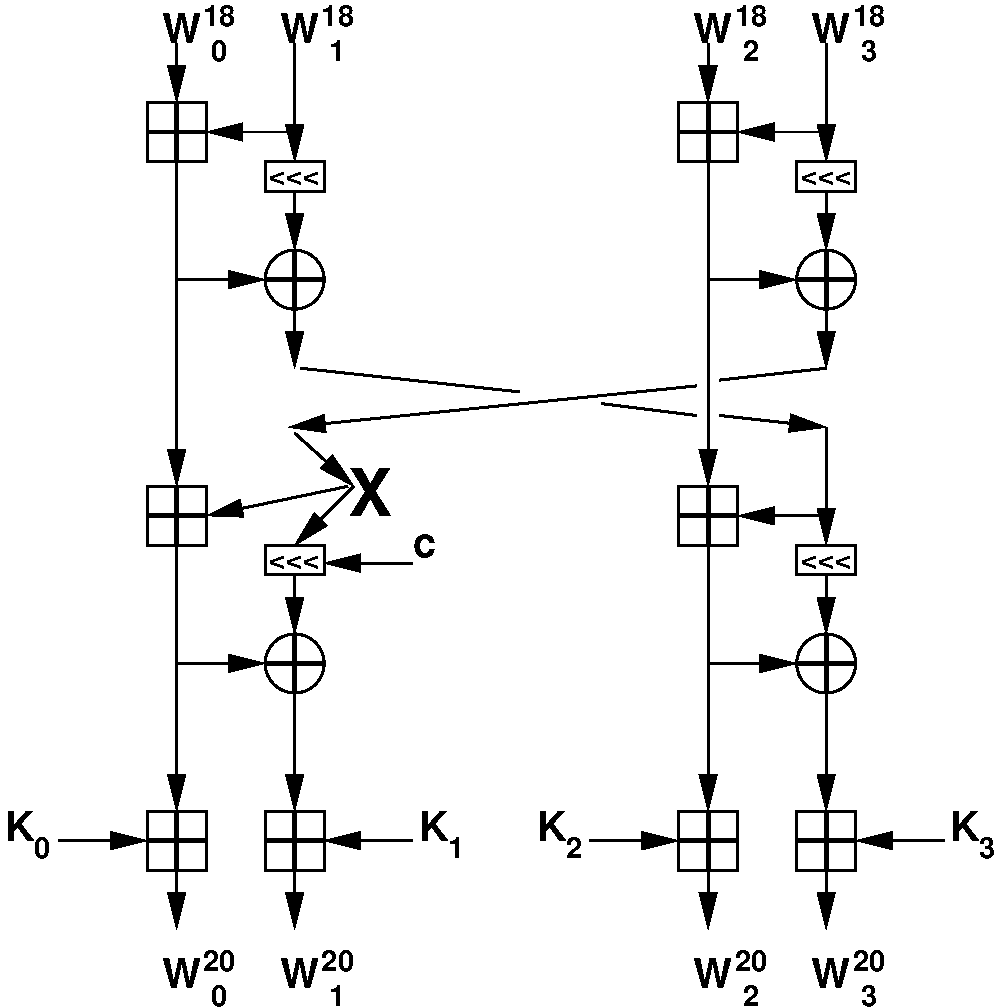
\includegraphics[width=0.45\textwidth]{key_recover.pdf}
 \caption{Simplified representation of rounds 19 and 20 of Threefish-256, including the key addition after round 20.}
 \label{fig:key-recovery}
\end{figure}

The $b$th bit $W^{18}_{1,0}$ of $W_1$ only depends on the key words $K_0, K_2, K_3$ and on the least significant $b$ bits of the intermediate variable \textbf{X}. For $i \in \{0, \ldots, b\}$, changing $X_{b-i}$ changes $W^{18}_{1,b}$ with probability $2^{-b}$. Similarly, changing $K_{1, (b-c-i-j)\bmod 64}$ only affects the bit $X_{b-i}$ with at most the probability $2^{-j}$. Thus, given $b$ and $c$, it is easy to decide which bits of $K_1$ are statistically relevant and must be guessed, and which bits of $K_1$ can safely be neglected.  Hence, we can employ our simple distinguisher to sort out most of the false guesses. This provides a key recovery attack for 20 rounds of Threefish-256.

For related reasons, we also don't need to guess all the bits of $K_0$, $K_2$ or $K_3$. We anticipate that it suffices to guess between 50\% and 75\% of all the 256 round key bits.

Threefish-512 and Threefish-1024 use longer keys, thus allowing an attack to spend more time without being slower than an exhaustive key search. We can exploit that to go beyond 20 rounds.

To analyze attacking any variant of Threefish with $r$ rounds, where $r \bmod 4 \neq 0$, we require an additional key addition after the final round. Otherwise, the final $r \bmod 4$ rounds could be trivially inverted, without knowing the key, and we could effectively attack $r-(r \bmod 4)$ rounds.
In the remainder of Section~\ref{sec:key-recovery}, we consider attacks on 21 rounds of Threefish-512 and 22 rounds of Threefish-1024, with a key addition after the final round. We assume that we can undo or neglect the ``regular'' key addition after round 20. Without this assumption, analyzing the partial decryption step becomes tricky.

\begin{itemize}
\item Threefish-512:  Assume the same kind of distinguisher as above, for 18 rounds.  Guess most of the final round key, which is added after round 21.  Partially decrypt rounds 21 to 19, and apply the distinguishing property to sort out false key guesses.

\item Threefish-1024: Assume a distinguisher for 18 rounds of Threefish-1024, partially decrypt rounds 22 to 20, and apply that distinguisher.
\end{itemize}

\subsubsection{Pushing the Attack Further: Prepending Four Additional Rounds}\label{sec:PushAttack}

To push the attack any further, we will look at the first few rounds of Threefish. In other words, we do the following:
\begin{itemize}
  \item Apply the above attack (on 20 rounds of Threefish-256, 21 rounds of 
    Threefish-512, and 22 rounds of Threefish-1024). But instead of
    starting with the first round, i.e., with round~0, we start with 
    round~4 now.
  \item To bridge the first four rounds, try an appropriate message
    difference as the input for round 0, which will get the input difference
    $D_5$ for round 5 that we need. (In our case, for any of the three
    Variants, this is $D_4 = (0, \ldots, 0, \delta)$ with $\delta=1000\ldots0
    \in \{0,1\}^{64}$).
  \item We cannot expect a probability-one approach here---even the best
    plaintext difference $D_0$ would only turn into the required difference
    $D_4$ with some probability $p_{0,\ldots,3}$. Thus, the values our
    distinguisher sees will be much more noisy. To compensate for the
    additional noise, we will have to increase the sample size by
    approximately a factor of $1/p^2_{0,\ldots,3}$. That is, if we needed
    $\sigma$ samples before, we now need $\sigma/p^2_{0,\ldots,3}$.
\end{itemize}
In other words, we need a good four-round differential characteristic with the output difference $D_4 = (0, \ldots, 0, \delta)$, which is then turned into an eight-round local collision from round 4 to round 11.

Consider a single round of Threefish.  If we want a specific difference $D_i$ after round $i$, we can run round $i$ backwards; in other words, in decryption direction, to compute some difference $D_{i-1}$ before round $i$. To analyze this attack, we need to estimate
\begin{itemize}
  \item the probability $p(D_{i-1} \rightarrow D_i)$ that two random
    inputs to round $i$ with difference $D_{i-1}$ produce any two outputs 
    with difference $D_i$, and
  \item the difference $D_{i-1}$ to maximize $p(D_{i-1} \rightarrow D_i)$.
\end{itemize}
We are only interested in a crude estimate of that probability. We will use the local Hamming weights to derive that estimate. Recall our MIX operation:
  \[ \mbox{Mix}_c(A,B) = (A+B, (B<\!<\!<c) \oplus (A+B). \]
If the Hamming weight is low, a good heuristic is to assume that the addition behaves exactly like the XOR operation. Assume Mix$_c(A,B)=(X,Y)$, and write $a$, $b$, $x$, and $y$ for the Hamming weights associated to $A$, $B$, $X$, and $Y$, respectively. For our crude estimate, we will apply the following three rules:
\begin{enumerate}
  \item $a = y+2x$.
  \item $b = x+y$.
  \item The differential probability is $\approx 2^{-x-y}$.
\end{enumerate}

Below, we will focus on Threefish-256, but we believe that this approach gives the adversary an additional four rounds for any of the three variants of Threefish.

Our target output difference is of the form $(0,0,0,\delta)$, with Hamming weight 1. The target output for the MIX operations in the final round are $(0,1)$ and $(0,0)$ (due to the permutation). Applying the above three rules provides an input difference with Hamming weights $(12,7,9,6)$, as depicted in figure~\ref{fig:reverserounds256}. Applying the third of our three rules, to estimate the probabilities of this differential behavior in every round, gives a probability of $2^{-21}$.
%
\begin{figure}[htbp]
  \centering
   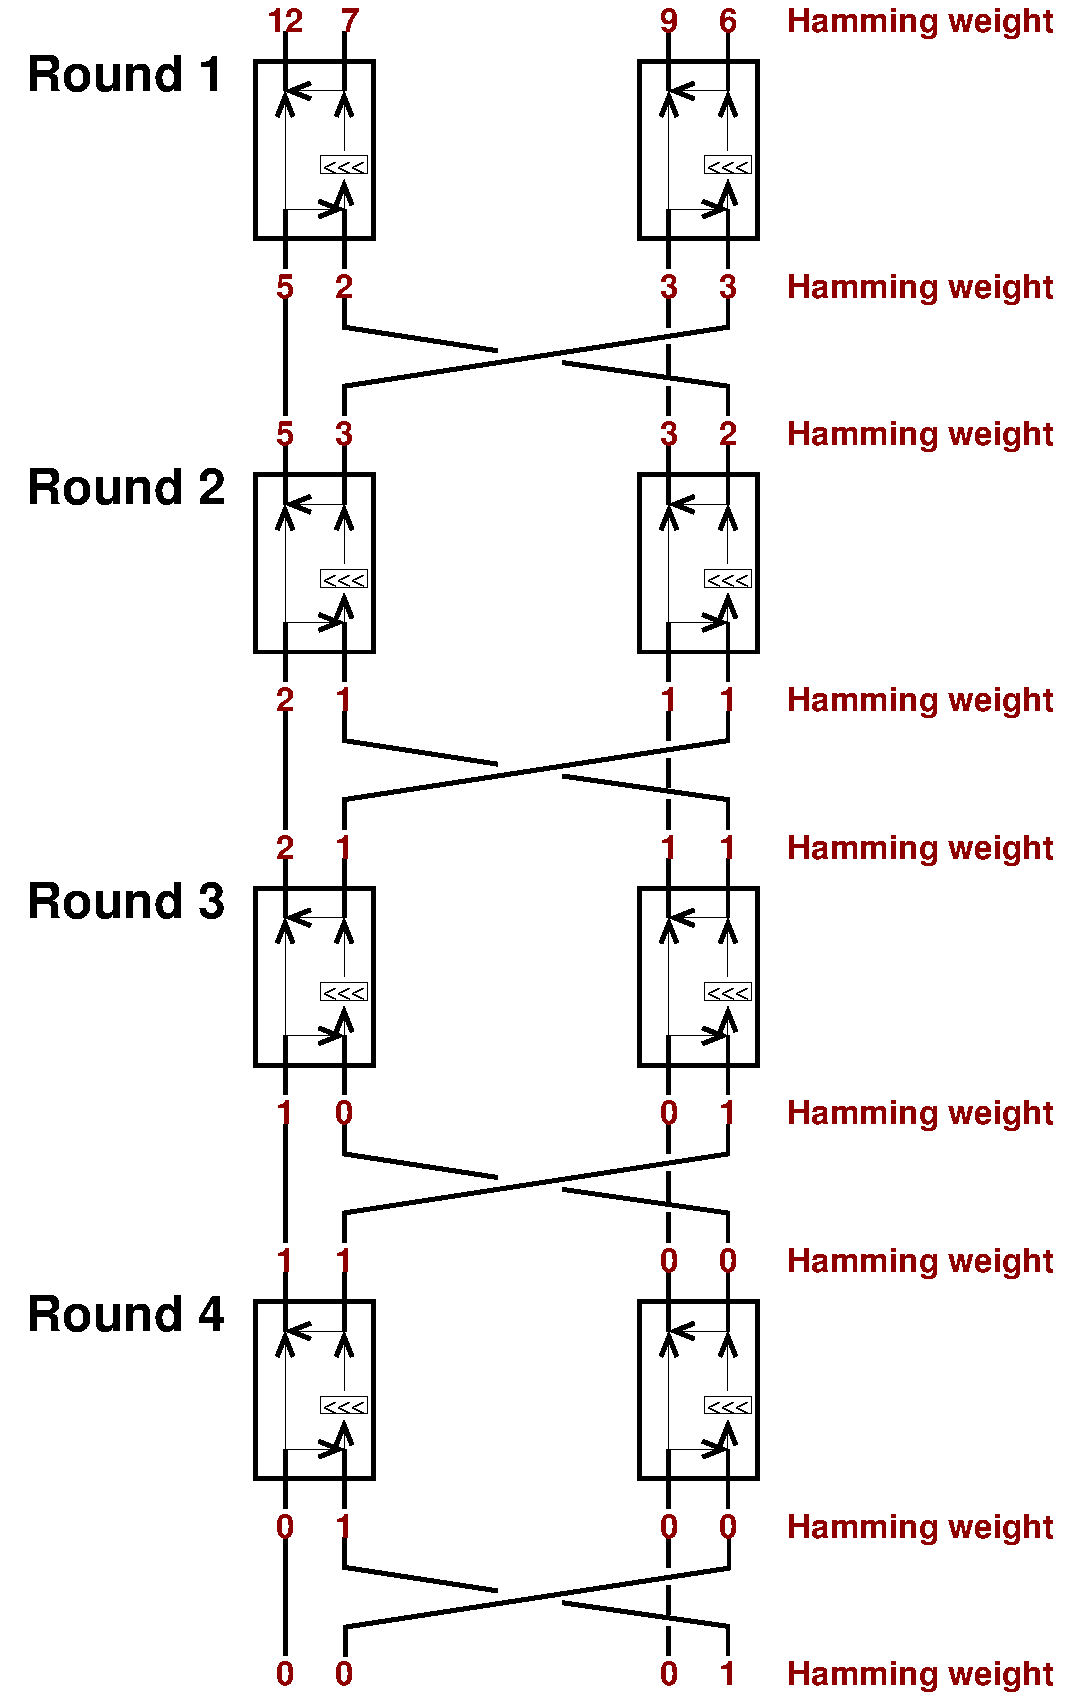
\includegraphics[width=0.45\textwidth]{reverserounds256.pdf}
  \caption{A differential characteristic for the first four rounds of
    Threefish-256.}
  \label{fig:reverserounds256}
\end{figure}

This allows an attacker to push distinguishing attacks and key recovery attacks four rounds further, at the cost of increasing the sample size by a factor of more than $2^{40}$. Our attacks apply for 24~rounds of Threefish-256, 25~rounds of Threefish-512, and 26~rounds of Threefish-1024.

Our probability estimate may be a bit too pessimistic, from the adversary's point of view. But the next logical step, namely, pushing the attack through another four rounds (one additional cycle), seems to require too large a sample size to be of any use for our key recovery attacks. 

\subsection{An Attack on the Threefish Block Cipher that Doesn't Quite Work} 

Our key schedule has been chosen with great care, such that the adversary cannot choose two different (tweak, cipher key) pairs with a zero difference in round $i$ and round $i+1$, or with a zero difference in round $i$ and $i+2$. In the first case, our local collision wouldn't break apart after eight rounds, but carry on for twelve rounds.

The case of a zero difference in round $i$ and $i+2$, with a nonzero difference in round $i+1$, is a bit more complicated, but instructive. We can mount a boomerang attack.%, as visualized in figure\ref{fig:boomerang}.

% Figure commented out for the time being.
% If Niels has time he'll draw a figure for a boomerang attack, but as this is well known in literature
% it is not of high importance.
%
%\begin{figure}[htbp]
%  \centering
%    \includegraphics[width=0.75\textwidth]{boomerang.pdf}
%  \caption{A boomerang distinguisher on Threefish, reduced to 32 rounds and
%    employing a weakened key schedule.}
%  \label{fig:boomerang}
%\end{figure}

Assume two key/tweak pairs $(K,T) \neq (K',T')$ with a zero difference in the second and the fourth subkeys. Choose related keys/tweaks and messages $M$ and $M'$, such that local collision in the first eight rounds occurs. That is, after eight rounds, before the key injection, we have the same intermediate value $I$, both when computing the encryption $E_{K,T}(M)$ and when computing the encryption $E_{K',T'}(M')$. After the key addition, we have a certain difference, and the next eight rounds can be expected to destroy any predictable difference. So we get two ciphertexts $C=E_{K,T}(M)$ and $C'=E_{K',T'}(M')$.

Now we choose new ciphertexts $C''$ and $C'''$ with the appropriate
differences, and decrypt $C''$ under $(K',T')$ and $C'''$ under $(K,T)$. In
rounds 9 to 16 (or rather, in rounds 16 to 9, when decrypting chosen ciphertext
queries), we get another local collision between $C''$ and $C$, and also a
local collision between $C'''$ and $C'$. Decrypting further, we get two
messages $M''=D_{K',T'}(C'')$ and $M'''=D_{K,T}(C''')$ with 
  \[ M'' \oplus M''' = M \oplus M'. \]
For an appropriately chosen difference, this holds with probability one.

Hence, with just two chosen-plaintext queries and another two chosen-ciphertext queries, we could easily distinguish 16 rounds of Threefish from a random permutation, using a boomerang property with probability one.

But recall that this attack requires a property that is not provided by our key schedule; namely, different key/tweak combinations with a zero difference in some subkey $i$ and a zero difference in subkey $i+2$.

Could it help the attacker if we got some key/tweak combinations in some subkey $i$ and $i+3$ or $i+4$? The boomerang property with probability one breaks apart, but a lower probability might still do. For example, assume a zero difference in subkeys $i$ and $i+4$. We would get a local collision for rounds 1--8, and then try to follow the most probable differential path to round 12 (with some probability $p_1 < 1$). From round 13 to round 16, we could try to find another most probable differential path, in order to exploit another local collision from round 17 to round 24. If everything worked out that way, we would get a boomerang distinguisher with the probability $p_1^2 \cdot p_2^2$.

To defend against that kind of boomerang attack, our key schedule ensures a distance between zero-difference subkeys of at least seven subkeys.

\subsection{Third-Party Cryptanalysis}
\label{sec:third-party-analysis}

Since the initial publication of the first version of this paper, many
researchers have spent time analyzing Threefish/Skein, and quite a few of
them have presented their results to the public. We are very pleased with this
development, but will not attempt to elaborate on all the results. 
Instead, we focus on the two most successful attempts to cryptanalyze
reduced-round Skein/Threefish, where ``success'' means maximizing the number
of rounds that can be attacked.

\subsubsection{Differential Cryptanalysis}


In September 2009, a group of six researchers published several attacks on reduced-round versions of Threefish, focusing on Threefish-512 \cite{ACMOPV09}. They managed to turn our 8-round pseudo-near-collisions with Hamming-weight 1 into a 17-round pseudo-near-collision, albeit with a much larger Hamming weight.  They also improved our related-key distinguisher for 17 rounds to 21 rounds, and presented related-key key-recovery attacks on 25 and 26 rounds of Threefish-512. The 26-round attack needs time $2^{507.8}$, just slightly faster than exhaustive search.  They also found a 21-round related-key impossible differential, a 32-round related-key boomerang key recovery attack, a 34-round related-key boomerang distinguisher, and a 35-round known-related-key boomerang distinguisher.

While these results specifically apply to the version of Threefish with the deprecated rotation
constants and the deprecated key schedule constant $C_5$, it is straightforward to use most of their ideas to analyze the current version of Threefish, with its new constants.  Indeed, one can understand how the attacks work without knowing the constants. 

The core of the 17-round pseudo-near-collision attack is the same eight-round local collision we used for our 8-round near-collision. To push the pseudo-near-collision from 8 to 17 rounds, the authors of \cite{ACMOPV09} prepend a 4-round differential trail with probability $2^{-33}$, and append a 5-round differential trail with probability $2^{-24}$. These trails were found by linearization; i.e., by treating the addition mod $2^{64}$ like an XOR and then computing the probability that it actually behaves like that. Adapting the attack to the constants just requires repeating the linearization step to find new differential trails, possibly with slightly different probabilities.

We used the eight-round local collision as a tool to build a 17-round distinguisher. Similarly, the authors of \cite{ACMOPV09} used their 17-round near-collision to build a 21-round distinguisher. To find a good distinguishing property, they ran a frequency test, searching for some highly biased bit---somewhat similar to our experiments in Section~\ref{sec:empiric512}. To deal with the new constants, one would essentially have to run a new frequency test. 

The paper's impossible differential employs a 13-round forward differential and a 7-round backward differential. For the forward differential, the first ten rounds do not depend on the constants, but the last three rounds do. Similarly, the last four rounds of the backward differential do not depend on the constants, but the first three do. It is not clear to us whether the impossible differential can be modified for the new rotation constants.

The paper's key-recovery attack improves our own key-recovery attack by means of a careful analysis---we only provided a sketch---and providing an improved search strategy that identifies and exploits neutral key bits. We believe the same approach would work for the new constants much as it works for the deprecated ones. One would need to rerun the frequency test to identify some bits with a significant bias. Since the attack workload for the 26-round attack is already close to an exhaustive key search, a slightly lower bias could possibly imply that the adapted attack would no longer be applicable for 26 rounds of Threefish-512, but it certainly remains applicable for 25 rounds. 

The paper also describes a boomerang property based on concatenating two differential trails. Each of these trails goes through some key-dependent rounds. In contrast to the trails for their local collision, the authors used a complex technique for finding good boomerang trails; namely, the Lipmaa-Moriai algorithms for finding good XOR-approximations for the addition modulo powers of two \cite{LiMo}. To deal with the new constants, one would have to run their software again, to calculate new differential trails. The probabilities of the new trails might vary slightly from the old trails' probabilities, but otherwise the boomerang property is the same. 

Exploiting a boomerang property for key-recovery, related-key, and known-related-key distinguishing is straightforward, regardless of the constants. 

The authors of \cite{ACMOPV09} presented some excellent ideas for analyzing
Threefish. Their analysis used the now-deprecated rotation constants and the
now-deprecated key schedule constant, but most of their attacks depend on the
structure of Threefish and on the key schedule---with the possible exception
of the impossible differential. We are confident one could easily adapt the
attacks to the current version of Threefish-512 and its new constants.

\subsubsection{Rotational Cryptanalysis}

The attacks presented in this section are obsolete. This is not the
cryptanalysts' fault; they did an excellent job. But since it turned
out that a very marginal tweak can defend against the very type of
attack that had been applied with the most success on Threefish/Skein, we
took the opportunity to apply that tweak; i.e., to change the key schedule
constant $C_5$ to $\TheConst$. The attacks seem to apply equally
well to either the deprecated or the new set of rotation constants. 

\medskip

{\bf Related-Key Key-Recovery.}
In early 2010, \cite{KN10} analyzed Threefish,
exploiting word-wise rotations. The attack is a related-key attack; i.e., there
is a secret key, unknown to the adversary, but the adversary can ask for the
encryptions of the plaintext under \emph{related} keys---here, specifically,
on keys where the same rotation is applied to each of the 64-bit words of the
key. 
%
Consider a plaintext
$P$, a key $K$, and a ciphertext $C=E_K(P)$, where $E$ is a reduced-round
version of a block cipher. Now apply a word-wise rotation to
each word of $P$ and $K$, to generate a new plaintext $\vec{P}$ and
$\vec{K}$. We also apply the same word-wise rotation on $C$ and get
$\vec{C}$. If there is any significant chance that 
   \begin{equation}\label{eq:rotational} 
     \vec{C} = E_{\vec{K}}(\vec{P}),
   \end{equation}
we can attack $E$ and even provide key recovery attacks for variants of the
same block cipher with slightly more rounds. 

Threefish is based three operations: addition, XOR, and rotate.
Neither XOR nor rotate have any effect on word-wise rotational properties:  
$\vec{X} \xor \vec{Y} = \vec{Z}$, where $Z= X \xor Y$, and for $Y=X \rol i$, 
$\vec{Y} = \vec{X} \rol i$. And even addition preserves word-wise
rotations with some significant probability. If $Z = X + Y$, then  
$\vec{Z}=\vec{X}+\vec{Y}$ holds with a probability $p=0.375$ for rotations by
1, $p=0.3125$ for rotations by 2, and $p \approx 0.25$ for rotations by large
amounts \cite{DaumThesis}. So the probability for Equation~\ref{eq:rotational}
to hold is $p^k$, where $k$ is the number of additions required
to compute $E_{\cdot}(\cdot)$.\footnote{This isn't precisely correct, since the
  probabilities that consecutive additions preserve a word-wise rotation don't need
  to be independent.}

Consider $E$\ =\ Threefish with the key schedule constant $C_5$. The adversary
will apply word-wise rotations by 2, so $p=0.3125$. (Without $C_5$, the
adversary could apply word-wise rotations by 1, thus improving $p$.)
Assume a version of Threefish with reduced rounds \emph{and} without the
subkey counter addition. In this case, the rotational attack is immediately
applicable, and \cite{KN10} claims attacks slightly faster than exhaustive
key search for 50 rounds of Threefish-256, Threefish-512, and
Threefish-1024. 

One of the purposes of the subkey counter addition was to prevent this type of
attack. Even a related-key attacker cannot apply a word-wise
rotate on the subkey counter. And if only one of two operands of an addition
or an XOR is rotated, while the second operand remains the same, then the
word-wise rotational property is destroyed. 
The main contribution of \cite{KN10} is to generate ``corrections'' $c_K$ and 
$c_p$ for  $\vec{K}$ and $\vec{P}$; i.e., instead of
Equation~\ref{eq:rotational}, they consider 
  \[ \vec{C} = E_{\vec{K}\oplus c_K}(\vec{P} \oplus c_P). \]
This approach depends heavily on the fact that the subkey counter is a tiny
value (4 bits for \cite{KN10}; a fifth bit would be needed in round 68 above) 
with a
low Hamming weight. Even when merely dealing with the tiny subkey counter, the
probability of success for the attack goes down considerably---as reflected by the
maximal number of rounds, which goes down from 50 to 42 rounds for
Threefish-512, from 50 to 39 rounds for Threefish-256, and from 50 to 44 rounds for
Threefish-1024, where the key addition at the end of round 44 is omitted. 

\medskip

{\bf Known-Key Distinguisher.}
Later in 2010, \cite{RKN10} extended this approach to a \emph{known-key
  distinguisher}. That is, there is no longer a secret key---the adversary is free
to choose both the key and the plaintext. Very informally, claiming a 
distinguisher means proving some nonrandom constellation of cipher
inputs/outputs, where generating a similar constellation for an ideal cipher
would need more work. In \cite{RKN10}, this means 
generating many equations of the form
  \[ \vec{C_i}  =  E_{\vec{K_i}\oplus c_K}(\vec{P_i}), \]
where $c_K$ is a ``correction'' and $C_i =E_{K_i}(P_i)$. 

Since known-key distinguishers provide the adversary with more degrees of 
freedom than related-key attacks, known-key distinguishers are often 
applicable to more rounds of a cipher or a hash function. In
the case of Threefish, \cite{RKN10} claim an attack for 53 rounds of
Threefish-256 and 57 rounds of Threefish-512. The workload for the attacks
is slightly below the exhaustive bound, which would be $2^{256}$ for
Threefish-256 and at $2^{512}$ for Threefish-512. (\cite{RKN10} did not
consider Threefish-1024.)

It seems possible to carry the approach from the Threefish block cipher to the
Skein hash function, though the adversary has fewer degrees of freedom and the
attack thus penetrates fewer rounds. 

We found the approach from \cite{RKN10} scientifically interesting, but were unsure of its relevance for Skein. What does it mean to show that certain
reduced-round variants of Threefish behave non-randomly in settings where all
or most inputs can be chosen \cite{RKN10}? For block ciphers, there is
currently no consensus in the cryptographic community. But for hash functions,
the consensus is that  behaving like an ideal hash function (a random
oracle) is vitally important. For this reason, 
we took care to prove Skein to be \emph{indifferentiable from a random
  oracle} if the compression function behaves randomly. In that light,
demonstrating that a reduced-round variant of Threefish---the core primitive
inside the Skein compression function---does not behave randomly is 
significant. However, the
indifferentiability proof for Skein (or rather, for the UBI mode) fails at the
birthday bound ($2^{128}$ for Skein-256 and $2^{256}$ for Skein-512); and, in
fact, there is a straightforward attack that only needs that amount of work.%
\footnote{%
  This is not a specific limitation of Skein---all hash functions 
  can be distinguished from random once an adversary has generated internal
  collisions, and generating such collisions for $s$ bits of state only needs 
  $2^{s/2}$ units of work.}
From our point of view, the really interesting question would be the
following: 
How many rounds can a known-key
  distinguisher penetrate with a workload below the birthday bound?
Unfortunately, the answer isn't provided in \cite{RKN10}.



\medskip

{\bf The effect of the tweak.}
Replacing $C_5$ by $C_{240}$ forces the attacker to provide ``corrections''
for 64-bit values, instead of for 4-bit values. If is still possible to
apply rotational attacks on reduced-round variants of Skein and Threefish. 
But the number of rounds must be reduced drastically. 


\subsection{Empirical Observations for Threefish with Random Rotation Constants}
\label{sec:random-constants}

After empirically studying the diffusion properties of the standard set of rotation constants, it may be interesting to also consider alternative choices for these constants. What would happen if we used random rotation constants, instead of our optimized constants? In other words, how critical is the choice of rotation constants for the security of Threefish? 

To explore this question, we performed the same empirical tests on several sets of random rotation constants that we did for our current set in Section~\ref{sec:related-key-attacks} and for the deprecated set in Section~\ref{sec:deprecatedrotconst}. For the sake of simplicity, we focused on Threefish-256. All experiments we describe in this section have been performed with a sample size of 25 million pairs. 

Similarly to Section~\ref{sec:related-key-attacks}, we performed our 
experiments using
Threefish with the old and now deprecated key schedule constant $C_5$ instead
of the new constant $\TheConst$. The research described in this section has
been motivated by the question of how far can we go by choosing apparently bad
sets of rotation constants until Threefish becomes insecure, and the new key
schedule constant is not expected to have any significant effect on this. 

Recall the following facts: 
\begin{enumerate}
 \item The rotation constants repeat every eight rounds.
 \item Each round of Threefish-256 employs two mix-operations.
 \item Each mix operation performs one addition, one XOR and one rotation. 
       That is, each mix operation requires one rotation constant.
\end{enumerate}
Thus, we can write the rotation constant as an eight-tuple of pairs of integers between 0 and 63. The original set of rotation constants for Threefish-256 is
    \[ \mbox{Threefish-256} := ((14,16), (52,57), (23,40), (5,37), 
                                (25,33), (46,12), (58,22), (32,32)). \]

Our experiments started with random rotation constants, derived from the decimal representation of $\pi$, $e$, and $\sqrt{2}$, respectively. We studied sets of rotation constants that repeat after eight rounds (as do the constants in Threefish) and four rounds.

The random rotation constants were only marginally less secure than the standard rotation constants, by providing somewhat better 17-round distinguishers.  As Table~\ref{tab:ObservationsRandom256} illustrates, none of these sets of rotation constants allowed us to distinguish more than 17 rounds (i.e., we could not identify any bit with a bias $>0.001$ in round 18), even those which repeated after four rounds.

\begin{table}[htbp]
  \centering
\begin{tabular}{|r|rrrr|r|}
\hline
round & \multicolumn{ 4}{c|}{\# bits with bias} & average\\
$r$ & \quad full & $>0.1$ & $>0.01$ & $>$ 0.001 & bias \\  \hline \hline
\multicolumn{6}{|l|}{Threefish-256 (standard constants)} \\ 
 16: &  0 &  3 &  41 &  63 & 0.00351  \\
 17: &  0 &  0 &  0 &  7 & 0.00012  \\
 18: &  0 &  0 &  0 &  0 & 0.00008  \\ \hline\hline
\multicolumn{6}{|l|}{consants derived from $\pi$ (repeats every 8 rounds)} \\ 
\multicolumn{6}{|l|}{((14,15), (35,32), (38,46), (26,43),
                      (38,32), (50,28), (19,39), (10,58))} \\ 
 16: &  0 &  6 &  42 &  67 & 0.00525  \\
 17: &  0 &  0 &  0 &  10 & 0.00013  \\
 18: &  0 &  0 &  0 &  0 & 0.00008  \\ \hline\hline
\multicolumn{6}{|l|}{constants derived from $e$ (repeats every 8 rounds)} \\
\multicolumn{6}{|l|}{((59,04), (52,35), (36,02), (47,13),
                      (52,24), (47,09), (36,62), (24,07))} \\
 16: &  0 &  20 &  67 &  95 & 0.01180  \\
 17: &  0 &  0 &  5 &  25 & 0.00039  \\
 18: &  0 &  0 &  0 &  0 & 0.00007  \\ \hline\hline
\multicolumn{6}{|l|}{constants derived from $\sqrt{2}$ (repeats every 8 rounds)} \\ 
\multicolumn{6}{|l|}{((41,42), (13,56), (23,09), (50,48),
                      (16,42), (09,56), (53,17), (24,46))} \\
 16: &  0 &  6 &  53 &  82 & 0.00579  \\
 17: &  0 &  0 &  3 &  12 & 0.00027  \\
 18: &  0 &  0 &  0 &  0 & 0.00008  \\ \hline\hline
\multicolumn{6}{|l|}{constants derived from $\pi$ (repeats every 4 rounds)} \\ 
\multicolumn{6}{|l|}{((14,15), (35,32), (38,46), (26,43)
                      (14,15), (35,32), (38,46), (26,43))} \\
 16: &  0 &  5 &  44 &  91 & 0.00524  \\
 17: &  0 &  0 &  0 &  10 & 0.00017  \\
 18: &  0 &  0 &  0 &  0 & 0.00008  \\ \hline\hline
\multicolumn{6}{|l|}{constants derived from $e$ (repeats every 4 rounds)} \\ 
\multicolumn{6}{|l|}{((59,04), (52,35), (36,02), (47,13),
                      (59,04), (52,35), (36,02), (47,13))} \\
 16: &  0 &  32 &  74 &  113 & 0.02048  \\
 17: &  0 &  3 &  16 &  33 & 0.00210  \\
 18: &  0 &  0 &  0 &  0 & 0.00008  \\ \hline\hline
\multicolumn{6}{|l|}{constants derived from $\sqrt{2}$ (repeats every 4 rounds)} \\ 
\multicolumn{6}{|l|}{((41,42), (13,56), (23,09), (50,48),
                      (41,42), (13,56), (23,09), (50,48))} \\
 16: &  0 &  10 &  55 &  93 & 0.00792  \\
 17: &  0 &  0 &  6 &  25 & 0.00052  \\
 18: &  0 &  0 &  0 &  0 & 0.00007  \\ \hline\hline
\end{tabular}
  \caption{Empirical results for variants of Threefish with random rotation constants,
           sample size 25,000,000~pairs.}
  \label{tab:ObservationsRandom256}
\end{table}

To improve the attacks, or rather, to weaken Threefish, we then considered random sets of rotation constants that repeated after two rounds. As shown in Table~\ref{tab:ObservationsTwoRepeat256}, this finally allowed us to improve the distinguisher to 18 and sometimes 19 rounds. One of our sets was ((17, 23), (32, 32), (17, 23), (32, 32),...), which we expected to perform worse than the others, as the effect of a rotation by 32 could cancel out two rounds later, when the next rotation by 32 takes place.%
\footnote{Studying such sets of rotation constants can be of interest, since these could possibly improve the performance of Threefish on 32-bit machines.} 
But even for this special case, we could not identify a distinguisher for more than 19 rounds. 

\begin{table}[htbp]
  \centering
\begin{tabular}{|r|rrrr|r|}
\hline
round & \multicolumn{ 4}{c|}{\# bits with bias} & average\\
$r$ & \quad full & $>0.1$ & $>0.01$ & $>$ 0.001 & bias \\  \hline \hline
\multicolumn{6}{|l|}{Threefish-256 (standard constants)} \\ 
 16: &  0 &  3 &  41 &  63 & 0.00351  \\
 17: &  0 &  0 &  0 &  7 & 0.00012  \\
 18: &  0 &  0 &  0 &  0 & 0.00008  \\
 \hline\hline
\multicolumn{6}{|l|}{constants derived from $\pi$ (repeats every 2 rounds)} \\ 
\multicolumn{6}{|l|}{((14,15), (35,32), (14,15), (35,32),
                      (14,15), (35,32), (14,15), (35,32))} \\ 
 16: &  0 &  94 &  127 &  154 & 0.08354  \\
 17: &  0 &  49 &  83 &  107 & 0.02986  \\
 18: &  0 &  4 &  33 &  56 & 0.00357  \\
 19: &  0 &  0 &  5 &  18 & 0.00035  \\
 20: &  0 &  0 &  0 &  0 & 0.00008  \\
 \hline\hline
\multicolumn{6}{|l|}{constants derived from $e$ (repeats every 2 rounds)} \\
\multicolumn{6}{|l|}{((59,04), (52,35), (59,04), (52,35),
                      (59,04), (52,35), (59,04), (52,35))} \\
 16: &  0 &  31 &  80 &  119 & 0.02318  \\
 17: &  0 &  3 &  20 &  43 & 0.00288  \\
 18: &  0 &  0 &  0 &  1 & 0.00008  \\
 19: &  0 &  0 &  0 &  0 & 0.00008  \\
 \hline\hline
\multicolumn{6}{|l|}{constants derived from $\sqrt{2}$ (repeats every 2 rounds)} \\ 
\multicolumn{6}{|l|}{((41,42), (13,56), (41,42), (13,56), 
                      (41,42), (13,56), (41,42), (13,56))} \\ 
 16: &  0 &  41 &  99 &  125 & 0.02551  \\
 17: &  0 &  4 &  28 &  70 & 0.00366  \\
 18: &  0 &  0 &  1 &  9 & 0.00016  \\
 19: &  0 &  0 &  0 &  0 & 0.00008  \\
 \hline\hline
\multicolumn{6}{|l|}{((17,23), (32,32), (17,23), (32,32),
                      (17,23), (32,32), (17,23), (32,32))} \\ 
 16: &  0 &  83 &  164 &  193 & 0.05918  \\
 17: &  0 &  26 &  73 &  130 & 0.01734  \\
 18: &  0 &  2 &  22 &  68 & 0.00193  \\
 19: &  0 &  0 &  0 &  8 & 0.00011  \\
 20: &  0 &  0 &  0 &  0 & 0.00007  \\
 \hline\hline
\end{tabular}
  \caption{Empirical results for variants of Threefish with rotation constants repeating every two rounds, sample size 25,000,000~pairs.}
  \label{tab:ObservationsTwoRepeat256}
\end{table}

In order to explore the limits of Threefish, we then tried to be even more malicious. 
Could we get improved distinguishers if we sabotaged Threefish by simply repeating the same rotation constant again and again? The surprising answer is that the random constants we tried---9, 14, 23, and 59---did not weaken Threefish nearly as much as we had expected. As shown in Table~\ref{tab:ObservationsRepeatSame}, we only found distinguishers for at most 26 rounds. Specific choices were worse,  For example, the constant 3 allowed for a 34-round distinguisher. And the constant 32 was as bad as we had anticipated: we could distinguish 40 rounds.

\begin{table}[htbp]
  \centering
\begin{tabular}{|r|rrrr|r|}
\hline
round & \multicolumn{ 4}{c|}{\# bits with bias} & average\\
$r$ & \quad full & $>0.1$ & $>0.01$ & $>$ 0.001 & bias \\ 
\hline\hline 
\multicolumn{6}{|l|}{constant 9} \\ 
\multicolumn{6}{|l|}{((09,09), (09,09), (09,09), (09,09),
                      (09,09), (09,09), (09,09), (09,09))} \\ 
 20: &  0 &  4 &  53 &  115 & 0.00448  \\
 21: &  0 &  0 &  11 &  66 & 0.00090  \\
 22: &  0 &  0 &  0 &  12 & 0.00014  \\
 23: &  0 &  0 &  0 &  0 & 0.00008  \\
\hline\hline
\multicolumn{6}{|l|}{constant 14} \\ 
\multicolumn{6}{|l|}{((14,14), (14,14), (14,14), (14,14), 
                      (14,14), (14,14), (14,14), (14,14))}\\
 20: &  0 &  12 &  65 &  112 & 0.00796  \\                                   
 21: &  0 &  1 &  25 &  68 & 0.00189  \\                                     
 22: &  0 &  0 &  3 &  25 & 0.00029  \\                                      
 23: &  0 &  0 &  0 &  0 & 0.00008  \\ 
\hline\hline
\multicolumn{6}{|l|}{constant 23} \\ 
\multicolumn{6}{|l|}{((23,23), (23,23), (23,23), (23,23),
	                    (23,23), (23,23), (23,23), (23,23))} \\ 
 22: &  0 &  4 &  40 &  74 & 0.00409  \\
 23: &  0 &  0 &  8 &  33 & 0.00057  \\
 24: &  0 &  0 &  0 &  13 & 0.00018  \\
 25: &  0 &  0 &  0 &  1 & 0.00008  \\
 26: &  0 &  0 &  0 &  0 & 0.00008  \\
\hline\hline
\multicolumn{6}{|l|}{constant 59} \\ 
\multicolumn{6}{|l|}{((59,59), (59,59), (59,59), (59,59),
                      (59,59), (59,59), (59,59), (59,59))} \\ 
 23: &  4 &  14 &  29 &  46 & 0.01614  \\
 24: &  0 &  4 &  23 &  37 & 0.00278  \\
 25: &  0 &  0 &  6 &  17 & 0.00041  \\
 26: &  0 &  0 &  0 &  2 & 0.00009  \\
 27: &  0 &  0 &  0 &  0 & 0.00008  \\
 \hline\hline\hline
\multicolumn{6}{|l|}{constant 3} \\ 
\multicolumn{6}{|l|}{((03,03), (03,03), (03,03), (03,03),
                      (03,03), (03,03), (03,03), (03,03))} \\ 
 31: &  0 &  12 &  32 &  58 & 0.00595  \\
 32: &  0 &  0 &  22 &  43 & 0.00167  \\
 33: &  0 &  0 &  4 &  29 & 0.00035  \\
 34: &  0 &  0 &  0 &  9 & 0.00011  \\
 35: &  0 &  0 &  0 &  0 & 0.00008  \\
 \hline\hline
\multicolumn{6}{|l|}{constant 32} \\ 
\multicolumn{6}{|l|}{((32,32), (32,32), (32,32), (32,32),
                      (32,32), (32,32), (32,32), (32,32))} \\ 
 33: &  0 &  4 &  52 &  86 & 0.00556  \\
 \multicolumn{6}{ c }{$\vdots$\hfill$\vdots$} \\
 38: &  0 &  0 &  0 &  27 & 0.00024  \\
 39: &  0 &  0 &  0 &  15 & 0.00014  \\
 40: &  0 &  0 &  0 &  2 & 0.00010  \\
 41: &  0 &  0 &  0 &  0 & 0.00009  \\
 \hline\hline
\end{tabular}
  \caption{Empirical results for variants of Threefish with a single rotation constant, sample size 25,000,000~pairs.}
  \label{tab:ObservationsRepeatSame}
\end{table}

It is possible to do even worse. Constant 0 would be trivially weak, since the least significant bits in all words are linear. Given our related-key differential, constant 63 would need at least from round 11 to round 74 to propagate the difference from the most significant bits to the least significant bits. Since the full cipher only has 72 rounds, attacking that variant of Threefish would also be easy. Constant 1 is not quite as bad as 0 or 63, but diffusion would still be very slow. We conjecture that related-key attacks against a Threefish-256 variant with one-bit rotations and 72 rounds would be practical. 

In summary, we searched for sets of rotation constants that would endanger or break Threefish.  The only such sets we could actually identify were \emph{obviously} malicious. Finding innocent-looking but dangerous sets of rotation constants for Threefish is still an open problem.

\subsection{Cryptanalysis Summary}

As our own cryptanalysis showed, it is feasible---in fact, quite easy---to create pseudo-near-collisions and pseudo-near-second-preimages for up to eight rounds of any variant of Skein; or rather, of the Skein compression function.  Here, ``near'' means Hamming-distance 2.  Using techniques similar to those from Section~\ref{sec:PushAttack}, one can push this from eight rounds to twelve rounds, at the cost of some significant but feasible amount of work. Assuming close to $2^n$ units of work, it may even be possible to find pseudo-near-second-preimages for up to sixteen rounds of the Skein-$n$ compression function, for all three versions of Skein.

We stress that none of these attacks are applicable to reduced-round versions of the Skein hash function.  Our current attacks only deal with reduced-round versions of the compression function.  Due to Skein's output transformation, it remains an open problem how to create collisions or second preimages for the Skein hash function, even if one can create pseudo-collisions or pseudo-second-preimages for the compression function.

We invite the reader to compare this to recent attacks on the security of the SHA-2 hash function family. The best implementable attacks on SHA-256 and SHA-512 we are aware of can generate collisions for up to 24 rounds of both SHA-256 and SHA-512 \cite{SS08a}. The time required for these attacks is between $2^{15.5}$ (for SHA-256, using a huge table for a speed-up trick) and $2^{32.5}$ (for SHA-512, without the huge table). As SHA-256 has 64 rounds and SHA-512 80 rounds, these attacks are a long way from actually endangering any member of the SHA-2 family. 

Regarding the Threefish block cipher, we have discussed attacks for Threefish reduced to 24 to 26 rounds. Namely, the attacks were for 24 rounds of Threefish-256 (full cipher: 72 rounds), 25 rounds of Threefish-512 (full cipher: 72 rounds), and 26 rounds of Threefish-1024 (full cipher: 80 rounds). As cryptosystem designers, we are driven by reasonable pessimism. These attacks depend on certain optimistic assumptions by the adversary. 

Additionally, we studied related-key boomerang attacks against Threefish, using a broken key schedule. For the broken variant, we described a probability-1 distinguisher for 16 rounds, and outlined how one might push this through a few more rounds when allowing smaller probabilities instead of probability 1. Because of the choice of our key schedule, one cannot actually apply these attacks to unmodified Threefish.

The authors of \cite{KN10,RKN10} contributed rotational attacks. By changing our
key schedule constant from $C_5$ to $\TheConst$, these attacks are no longer
applicable to Threefish or Skein.

The authors of \cite{ACMOPV09} presented some interesting ideas to improve the cryptanalysis of Threefish. Their best chosen-plaintext related-key key-recovery attack works for 26 rounds of Threefish-512, improving on our own conjectured attack by one round. Their best chosen plaintext/chosen ciphertext key-recovery attack is a boomerang attack on 32 rounds of Threefish-512. They extend this to a known-related-key distinguisher for 35 rounds. These attacks mostly exploit the Threefish structure and properties of the key schedule. One can adapt their observations and attacks to the new constants, with the possible exception of the impossible differential attack. In some cases, the adaptation may slightly change the number of rounds for which the attacks can be applied.  

For comparison, consider the current state of cryptanalysis withh the
current state for the SHA-2 family.  As far as we know, the best
attack on SHACAL-2, the block cipher inside SHA-256, penetrates 44
rounds \cite{LK08}---more than two-thirds of the full 64 rounds.
However, since it requires $2^{233}$ related-key chosen plaintexts and
time $2^{497.2}$, the attack is entirely academic.  It is based on the
related-key rectangle attack scenario, using a probability $2^{-460}$
distinguisher for 35 rounds of SHACAL-2. Note that related-key
rectangle attacks are close relatives to related-key boomerang
attacks, considered by ourselves and in \cite{ACMOPV09}, for modified
Threefish.


\section{Skein Website}
\label{sec:website}

The Skein website is \purl{http://www.skein-hash.info/}.  In addition to the latest version of this paper, the website contains reference code, optimized code, and code to generate performance measurements, test vectors, and known answer tests.  We will continue to update the page with additional security proofs, cryptanalysis results, performance measurements, implementations, and so on.

The website is always the source for the most up-to-date version of this paper, and the most up-to-date information about Skein.

\section{Legal Disclaimer}

To the best of our knowledge, neither the Skein hash function, the Threefish block cipher, the UBI hashing mode, nor our optional argument system, are encumbered by any patents.  We have not, and will not, apply for patents on any part of our design or anything in this document, and we are unaware of any other patents or patent filings that cover this work. The example source code---and all other code on the Skein website---is in the public domain and can be freely used.

We make this submission to NIST's hash function competition solely as individuals.  Our respective employers neither endorse nor condemn this submission.

\section{Acknowledgements}

We would like to thank NIST for overseeing this competition, and our employers for allowing us the time to work on this submission.  We would also like to thank the external reviewers who analyzed our algorithm when it was in draft---Frederik Armknecht, Martin Cochran, Hal Finney, Gary Graunke, Susan Landau, Sascha M\"uller-Lobeck, Kerry McKay, and Ray Savarda---and the following students of Stefan Lucks: Ewan Fleischmann, Christian Forler, Michael Gorski, Dennis Hoppe, Martin Kausche, Stoyan Stoyanov, and Julian Seifert. Also Beth Friedman for editing the submission document with Sue Heim's valuable suggestions.  And finally, we would like to thank our respective families for putting up with all of the time and attention this project required.

\section{About the Authors}

The Skein team is essentially a group of friends. We've all worked on cryptography and cryptographic engineering for many years.  We've met and worked together many times; our team includes half of the Twofish team \cite{Twofish}. Our experiences are extensive and diverse, which was a great help in bringing all aspects of the design together. It also led to some very interesting discussions: a single e-mail thread might span mathematical proofs, PR, and political considerations, and discussions on how modern CPUs work. We had lots of fun.

We realize our affiliations read like a powerful industry consortium, but we are not.  Our employers kindly agreed to let us do this work, but most of it was done on our own time.  Really, they only have the vaguest idea what we're doing.

\appendix
% I don't know why we need the \leavevmode, but the section heading gets swallowed otherwise
\clearpage \leavevmode

%
% Ugly hack to put "Appendix" in front of each appendix letter in the text
%
\begingroup
\makeatletter
\renewcommand\section{\@startsection {section}{1}{\z@ Appendix }%
                                   {-3.5ex \@plus -1ex \@minus -.2ex}%
                                   {2.3ex \@plus.2ex}%
                                   {\normalfont\Large\bfseries}}
\makeatother

\section{Overview of Symbols}

This appendix gives an overview and index of the symbols used in the definition of Skein.

\begin{list}{?}{%
\parsep = \parskip
\itemsep = 0.5ex plus .5ex minus 0.2 ex
\leftmargin = 27 mm
\rightmargin = 0cm
\listparindent = \parindent
\labelsep = 2 mm
\labelwidth = 25 mm
\renewcommand{\makelabel}[1]{$#1$\hfill}
}

\item[\BytesToWords] A function that converts a string of bytes to a string of 64-bit words.
    \symdefref{BytesToWords}.

\item[C]    The Threefish ciphertext \symdefref{C} or the configuration string \symdefref{Conf}.

\item[c_i]  The words of ciphertext $C$. \symdefref{c_i}

\item[e_{d,i}] The $i$th word of the result of the subkey addition (if any) in round $d$. \symdefref{e_di}

\item[d]    The round number. \symdefref{d}

\item[f_{d,i}] The $i$th word of the result of the MIX functions in round $d$. \symdefref{f_di}

\item[G_i]  Chaining values between different UBI invocations. \symdefref{G_i}

\item[H_i]  Chaining values used within a UBI computation. \symdefref{H_i}

\item[K]    The key, either the Threefish key \symdefref{Threefish-K} or the Skein key. \symdefref{Skein-K}

\item[K']    The processed key that starts the Skein UBI chain. \symdefref{Kprime}

\item[k_i]  The words of the Threefish key $K$. \symdefref{k_i}

\item[k_{s,i}] The words of subkey $s$. \symdefref{k_si}

\item[M]    Used for various message strings.

\item[M_i]  Block $i$ of message string $M$.

\item[N_b]  The number of bytes in the state. \symdefref{N_b}

\item[N_o]  The number of output bits of Skein. \symdefref{N_o}

\item[N_r]  The number of rounds in Threefish. \symdefref{N_r}

\item[N_w]  The number of words in the state. \symdefref{N_w}

\item[P]    The plaintext input to Threefish. \symdefref{P}

\item[p_i]  The words of plaintext $P$. \symdefref{p_i}

\item[\pi(i)] The permutation applied to the state words in each round. \symdefref{pi}

\item[R_{d,j}] The rotation constant for mix $j$ in round $d$. \symdefref{R_dj}

\item[s]    The subkey number. \symdefref{s}

\item[T]    The tweak value. \symdefref{T}

\item[T_s]  The starting tweak value for UBI. \symdefref{T_s}

\item[T_\text{xxx}] Various type value constants. \symdefref{T_xxx}

\item[t_i]  The words of tweak $T$. \symdefref{t_i}

\item[\ToBytes] A function that converts an integer to a string of bytes, LSB first. \symdefref{ToBytes}

\item[\ToInt]   A function that converts a string of bytes to an integer, LSB first. \symdefref{ToInt}

\item[v_{d,i}] The value of the $i$th word of the Threefish encryption state after $d$ rounds. \symdefref{v_di}

\item[\WordsToBytes] A function that converts a string of 64-bit words to a string of bytes. \symdefref{WordsToBytes}

\item[(x_0, x_1)] The inputs to a MIX function. \symdefref{x0x1}

\item[Y_f]  Encoding of the fan-out for tree hashing. \symdefref{Y_f}

\item[Y_l]  Encoding of the leaf node size for tree hashing. \symdefref{Y_l}

\item[Y_m]  Maximum tree height for tree hashing. \symdefref{Y_m}

\item[(y_0, y_1)] The outputs of a MIX function. \symdefref{y0y1}

\end{list}


\section{Initial Chaining Values}\label{sec:initialchainingvalues}

These are the IV values for the configurations in Table~\ref{tab:versions}.  These constants are the output of the configuration UBI.  If you are using Skein as a normal hash function, you can use these IV values as constants and skip the configuration step entirely.  Note that these are 64-bit words, not byte strings.

\subsection{Skein-256-128}
\begin{verbatim}
0xE1111906964D7260, 0x883DAAA77C8D811C, 0x10080DF491960F7A, 0xCCF7DDE5B45BC1C2
\end{verbatim}

\subsection{Skein-256-160}
\begin{verbatim}
0x1420231472825E98, 0x2AC4E9A25A77E590, 0xD47A58568838D63E, 0x2DD2E4968586AB7D
\end{verbatim}

\subsection{Skein-256-224}
\begin{verbatim}
0xC6098A8C9AE5EA0B, 0x876D568608C5191C, 0x99CB88D7D7F53884, 0x384BDDB1AEDDB5DE
\end{verbatim}

\subsection{Skein-256-256}
\begin{verbatim}
0xFC9DA860D048B449, 0x2FCA66479FA7D833, 0xB33BC3896656840F, 0x6A54E920FDE8DA69
\end{verbatim}

\subsection{Skein-512-128}
\begin{verbatim}
0xA8BC7BF36FBF9F52, 0x1E9872CEBD1AF0AA, 0x309B1790B32190D3, 0xBCFBB8543F94805C
0x0DA61BCD6E31B11B, 0x1A18EBEAD46A32E3, 0xA2CC5B18CE84AA82, 0x6982AB289D46982D
\end{verbatim}

\subsection{Skein-512-160}
\begin{verbatim}
0x28B81A2AE013BD91, 0xC2F11668B5BDF78F, 0x1760D8F3F6A56F12, 0x4FB747588239904F
0x21EDE07F7EAF5056, 0xD908922E63ED70B8, 0xB8EC76FFECCB52FA, 0x01A47BB8A3F27A6E
\end{verbatim}

\subsection{Skein-512-224}
\begin{verbatim}
0xCCD0616248677224, 0xCBA65CF3A92339EF, 0x8CCD69D652FF4B64, 0x398AED7B3AB890B4
0x0F59D1B1457D2BD0, 0x6776FE6575D4EB3D, 0x99FBC70E997413E9, 0x9E2CFCCFE1C41EF7
\end{verbatim}

\subsection{Skein-512-256}
\begin{verbatim}
0xCCD044A12FDB3E13, 0xE83590301A79A9EB, 0x55AEA0614F816E6F, 0x2A2767A4AE9B94DB
0xEC06025E74DD7683, 0xE7A436CDC4746251, 0xC36FBAF9393AD185, 0x3EEDBA1833EDFC13
\end{verbatim}

\subsection{Skein-512-384}
\begin{verbatim}
0xA3F6C6BF3A75EF5F, 0xB0FEF9CCFD84FAA4, 0x9D77DD663D770CFE, 0xD798CBF3B468FDDA
0x1BC4A6668A0E4465, 0x7ED7D434E5807407, 0x548FC1ACD4EC44D6, 0x266E17546AA18FF8
\end{verbatim}

\subsection{Skein-512-512}
\begin{verbatim}
0x4903ADFF749C51CE, 0x0D95DE399746DF03, 0x8FD1934127C79BCE, 0x9A255629FF352CB1
0x5DB62599DF6CA7B0, 0xEABE394CA9D5C3F4, 0x991112C71A75B523, 0xAE18A40B660FCC33
\end{verbatim}

\subsection{Skein-1024-384}
\begin{verbatim}
0x5102B6B8C1894A35, 0xFEEBC9E3FE8AF11A, 0x0C807F06E32BED71, 0x60C13A52B41A91F6
0x9716D35DD4917C38, 0xE780DF126FD31D3A, 0x797846B6C898303A, 0xB172C2A8B3572A3B
0xC9BC8203A6104A6C, 0x65909338D75624F4, 0x94BCC5684B3F81A0, 0x3EBBF51E10ECFD46
0x2DF50F0BEEB08542, 0x3B5A65300DBC6516, 0x484B9CD2167BBCE1, 0x2D136947D4CBAFEA
\end{verbatim}

\subsection{Skein-1024-512}
\begin{verbatim}
0xCAEC0E5D7C1B1B18, 0xA01B0E045F03E802, 0x33840451ED912885, 0x374AFB04EAEC2E1C
0xDF25A0E2813581F7, 0xE40040938B12F9D2, 0xA662D539C2ED39B6, 0xFA8B85CF45D8C75A
0x8316ED8E29EDE796, 0x053289C02E9F91B8, 0xC3F8EF1D6D518B73, 0xBDCEC3C4D5EF332E
0x549A7E5222974487, 0x670708725B749816, 0xB9CD28FBF0581BD1, 0x0E2940B815804974
\end{verbatim}

\subsection{Skein-1024-1024}
\begin{verbatim}
0xD593DA0741E72355, 0x15B5E511AC73E00C, 0x5180E5AEBAF2C4F0, 0x03BD41D3FCBCAFAF
0x1CAEC6FD1983A898, 0x6E510B8BCDD0589F, 0x77E2BDFDC6394ADA, 0xC11E1DB524DCB0A3
0xD6D14AF9C6329AB5, 0x6A9B0BFC6EB67E0D, 0x9243C60DCCFF1332, 0x1A1F1DDE743F02D4
0x0996753C10ED0BB8, 0x6572DD22F2B4969A, 0x61FD3062D00A579A, 0x1DE0536E8682E539
\end{verbatim}

\section{Test Vectors}\label{sec:testvectors}

\subsection{Skein-256-256}

\begin{verbatim}
Message data:
     FF

Result:
     0B 98 DC D1 98 EA 0E 50 A7 A2 44 C4 44 E2 5C 23
     DA 30 C1 0F C9 A1 F2 70 A6 63 7F 1F 34 E6 7E D2
							 			 
Message data:				 			 
     FF FE FD FC FB FA F9 F8 F7 F6 F5 F4 F3 F2 F1 F0
     EF EE ED EC EB EA E9 E8 E7 E6 E5 E4 E3 E2 E1 E0
							 			 
Result:						 			 
     8D 0F A4 EF 77 7F D7 59 DF D4 04 4E 6F 6A 5A C3
     C7 74 AE C9 43 DC FC 07 92 7B 72 3B 5D BF 40 8B
							 			 
Message data:				 			 
     FF FE FD FC FB FA F9 F8 F7 F6 F5 F4 F3 F2 F1 F0
     EF EE ED EC EB EA E9 E8 E7 E6 E5 E4 E3 E2 E1 E0
     DF DE DD DC DB DA D9 D8 D7 D6 D5 D4 D3 D2 D1 D0
     CF CE CD CC CB CA C9 C8 C7 C6 C5 C4 C3 C2 C1 C0

Result:
     DF 28 E9 16 63 0D 0B 44 C4 A8 49 DC 9A 02 F0 7A
     07 CB 30 F7 32 31 82 56 B1 5D 86 5A C4 AE 16 2F
\end{verbatim}

\subsection{Skein-512-512}

\begin{verbatim}

Message data:
     FF

Result:
     71 B7 BC E6 FE 64 52 22 7B 9C ED 60 14 24 9E 5B
     F9 A9 75 4C 3A D6 18 CC C4 E0 AA E1 6B 31 6C C8
     CA 69 8D 86 43 07 ED 3E 80 B6 EF 15 70 81 2A C5
     27 2D C4 09 B5 A0 12 DF 2A 57 91 02 F3 40 61 7A

Message data:
     FF FE FD FC FB FA F9 F8 F7 F6 F5 F4 F3 F2 F1 F0
     EF EE ED EC EB EA E9 E8 E7 E6 E5 E4 E3 E2 E1 E0
     DF DE DD DC DB DA D9 D8 D7 D6 D5 D4 D3 D2 D1 D0
     CF CE CD CC CB CA C9 C8 C7 C6 C5 C4 C3 C2 C1 C0

Result:
     45 86 3B A3 BE 0C 4D FC 27 E7 5D 35 84 96 F4 AC
     9A 73 6A 50 5D 93 13 B4 2B 2F 5E AD A7 9F C1 7F
     63 86 1E 94 7A FB 1D 05 6A A1 99 57 5A D3 F8 C9
     A3 CC 17 80 B5 E5 FA 4C AE 05 0E 98 98 76 62 5B

Message data:
     FF FE FD FC FB FA F9 F8 F7 F6 F5 F4 F3 F2 F1 F0
     EF EE ED EC EB EA E9 E8 E7 E6 E5 E4 E3 E2 E1 E0
     DF DE DD DC DB DA D9 D8 D7 D6 D5 D4 D3 D2 D1 D0
     CF CE CD CC CB CA C9 C8 C7 C6 C5 C4 C3 C2 C1 C0
     BF BE BD BC BB BA B9 B8 B7 B6 B5 B4 B3 B2 B1 B0
     AF AE AD AC AB AA A9 A8 A7 A6 A5 A4 A3 A2 A1 A0
     9F 9E 9D 9C 9B 9A 99 98 97 96 95 94 93 92 91 90
     8F 8E 8D 8C 8B 8A 89 88 87 86 85 84 83 82 81 80

Result:
     91 CC A5 10 C2 63 C4 DD D0 10 53 0A 33 07 33 09
     62 86 31 F3 08 74 7E 1B CB AA 90 E4 51 CA B9 2E
     51 88 08 7A F4 18 87 73 A3 32 30 3E 66 67 A7 A2
     10 85 6F 74 21 39 00 00 71 F4 8E 8B A2 A5 AD B7

\end{verbatim}

\subsection{Skein-1024-1024}

\begin{verbatim}

Message data:
     FF

Result:
     E6 2C 05 80 2E A0 15 24 07 CD D8 78 7F DA 9E 35
     70 3D E8 62 A4 FB C1 19 CF F8 59 0A FE 79 25 0B
     CC C8 B3 FA F1 BD 24 22 AB 5C 0D 26 3F B2 F8 AF
     B3 F7 96 F0 48 00 03 81 53 1B 6F 00 D8 51 61 BC
     0F FF 4B EF 24 86 B1 EB CD 37 73 FA BF 50 AD 4A
     D5 63 9A F9 04 0E 3F 29 C6 C9 31 30 1B F7 98 32
     E9 DA 09 85 7E 83 1E 82 EF 8B 46 91 C2 35 65 65
     15 D4 37 D2 BD A3 3B CE C0 01 C6 7F FD E1 5B A8

Message data:
     FF FE FD FC FB FA F9 F8 F7 F6 F5 F4 F3 F2 F1 F0
     EF EE ED EC EB EA E9 E8 E7 E6 E5 E4 E3 E2 E1 E0
     DF DE DD DC DB DA D9 D8 D7 D6 D5 D4 D3 D2 D1 D0
     CF CE CD CC CB CA C9 C8 C7 C6 C5 C4 C3 C2 C1 C0
     BF BE BD BC BB BA B9 B8 B7 B6 B5 B4 B3 B2 B1 B0
     AF AE AD AC AB AA A9 A8 A7 A6 A5 A4 A3 A2 A1 A0
     9F 9E 9D 9C 9B 9A 99 98 97 96 95 94 93 92 91 90
     8F 8E 8D 8C 8B 8A 89 88 87 86 85 84 83 82 81 80

Result:
     1F 3E 02 C4 6F B8 0A 3F CD 2D FB BC 7C 17 38 00
     B4 0C 60 C2 35 4A F5 51 18 9E BF 43 3C 3D 85 F9
     FF 18 03 E6 D9 20 49 31 79 ED 7A E7 FC E6 9C 35
     81 A5 A2 F8 2D 3E 0C 7A 29 55 74 D0 CD 7D 21 7C
     48 4D 2F 63 13 D5 9A 77 18 EA D0 7D 07 29 C2 48
     51 D7 E7 D2 49 1B 90 2D 48 91 94 E6 B7 D3 69 DB
     0A B7 AA 10 6F 0E E0 A3 9A 42 EF C5 4F 18 D9 37
     76 08 09 85 F9 07 57 4F 99 5E C6 A3 71 53 A5 78

Message data:
     FF FE FD FC FB FA F9 F8 F7 F6 F5 F4 F3 F2 F1 F0
     EF EE ED EC EB EA E9 E8 E7 E6 E5 E4 E3 E2 E1 E0
     DF DE DD DC DB DA D9 D8 D7 D6 D5 D4 D3 D2 D1 D0
     CF CE CD CC CB CA C9 C8 C7 C6 C5 C4 C3 C2 C1 C0
     BF BE BD BC BB BA B9 B8 B7 B6 B5 B4 B3 B2 B1 B0
     AF AE AD AC AB AA A9 A8 A7 A6 A5 A4 A3 A2 A1 A0
     9F 9E 9D 9C 9B 9A 99 98 97 96 95 94 93 92 91 90
     8F 8E 8D 8C 8B 8A 89 88 87 86 85 84 83 82 81 80
     7F 7E 7D 7C 7B 7A 79 78 77 76 75 74 73 72 71 70
     6F 6E 6D 6C 6B 6A 69 68 67 66 65 64 63 62 61 60
     5F 5E 5D 5C 5B 5A 59 58 57 56 55 54 53 52 51 50
     4F 4E 4D 4C 4B 4A 49 48 47 46 45 44 43 42 41 40
     3F 3E 3D 3C 3B 3A 39 38 37 36 35 34 33 32 31 30
     2F 2E 2D 2C 2B 2A 29 28 27 26 25 24 23 22 21 20
     1F 1E 1D 1C 1B 1A 19 18 17 16 15 14 13 12 11 10
     0F 0E 0D 0C 0B 0A 09 08 07 06 05 04 03 02 01 00

Result:
     84 2A 53 C9 9C 12 B0 CF 80 CF 69 49 1B E5 E2 F7
     51 5D E8 73 3B 6E A9 42 2D FD 67 66 65 B5 FA 42
     FF B3 A9 C4 8C 21 77 77 95 08 48 CE CD B4 8F 64
     0F 81 FB 92 BE F6 F8 8F 7A 85 C1 F7 CD 14 46 C9
     16 1C 0A FE 8F 25 AE 44 4F 40 D3 68 00 81 C3 5A
     A4 3F 64 0F D5 FA 3C 3C 03 0B CC 06 AB AC 01 D0
     98 BC C9 84 EB D8 32 27 12 92 1E 00 B1 BA 07 D6
     D0 1F 26 90 70 50 25 5E F2 C8 E2 4F 71 6C 52 A5
\end{verbatim}

\section{NIST SHA-3 Round 2 Tweak: Rotation Constants}\label{sec:tweakrotconst}

This specification of Skein includes a ``tweak'' for Round 2 of the NIST SHA-3 competition: the rotation constants shown in Table~\ref{tab:rotations}, which differ from those originally submitted to NIST in October 2008 \cite{Skein1}. All existing and future implementations of Skein \emph{must} now use these new rotation constants to be compliant. Changing the rotation constants required updating all the Skein test vectors
(Appendix~\ref{sec:testvectors}) and the precomputed initial chaining values
(Appendix~\ref{sec:initialchainingvalues}).

Some comments are in order about the tweak. It is our belief is that the structure of Threefish would be secure with almost any randomly chosen set of rotation constants (see Section~\ref{sec:random-constants}). Indeed, it would give us pause if a randomly generated set of rotation constants were to result in an attack.

Nonetheless, given that we have an opportunity to select the rotation constants, it makes sense to maximize diffusion as much as possible. In the original NIST submission, we had limited time to design and run a search algorithm for rotation constants. Some time after the initial submission, Guillaume Sevestre contacted us \cite{Sev09} with a suggestion for a new search algorithm---the evolutionary algorithm described in Section~\ref{sec:threefishdesign}---which indeed produced significantly better results using the original diffusion metric. Many thanks are due to Guillaume for collaborating at length to educate us on the new search algorithm and how to optimize it.

In addition, the metric used in the original search (see the definition of $H_{min}$ in Section~\ref{sec:deprecatedrotconst}) was not the most appropriate value to optimize.  This metric minimized the probability that a particular input bit flip would \emph{not} trigger a particular output bit flip, but it did not attempt to minimize the probability such a bit flip \emph{would} occur. A slightly different metric, minimizing the maximum bias from $K/2$ in the histogram, was more consistent with what we were trying to achieve. Not surprisingly, we found that some of the original rotation constant sets resulted in rather poor values of the maximum bias due to cases where the output bit almost always flipped for a given input bit difference.  Again, we do not expect that this bias using the original rotation constants would result in an attack, but as long as we were considering a tweak, it seemed best to use the bias as the new search metric. 

When we ran the new search algorithm for two days using the improved bias metric, the gains in both diffusion metrics were generally impressive. A comparison is given in Table~\ref{tab:rotbiascomparison}, with the bias listed as the maximum deviation from $0.5$ of the value $x = h_i/K$ across the entire histogram, where $h_i$ is an entry in the histogram.  Thus, a smaller value in the table indicates better diffusion, and the worst possible value (i.e., 0.50) would indicate that at least one output bit location \emph{never} (or always) changed for a given input bit difference. Again, the original bias metric only took into account values of $x < 0.5$, while the new metric includes both positive and negative deviations, so bias values obtained using the old metric will never be larger than those using the new metric. Note that a later six-day search improved the metric by only about 0.002 for Skein-256, 0.007 for Skein-512, and 0.014 for Skein-1024 over the two-day results (i.e., t
hose in Table~\ref{tab:rotations}), so we are comfortable using the latter.


\begin{table}[htb]
  \begin{center}
    \begin{tabular}{|l|c|c|c|}
    \hline
    & \multicolumn{3}{c|}{Rotation Constants}  \\ \cline{2-4}
    & \multicolumn{2}{c|}{Old Set} & New Set   \\ \cline{2-4}
    & Old Metric & New Metric & New Metric     \\
	\hline
    Skein-256  & 0.10  &  0.24  & 0.09  \\
    Skein-512  & 0.33  &  0.48  & 0.25  \\
    Skein-1024 & 0.26  &  0.35  & 0.15  \\
    \hline
    \end{tabular}
   \end{center}\caption{Maximum observed bias for $K=16384$}
  \label{tab:rotbiascomparison}
\end{table}

Given these two results and the fact that NIST has allowed tweaks at this point in the competition, we feel it would be somewhat irresponsible \emph{not} to submit the improved rotation constant set. However, if NIST decides for some reason that changing the Skein rotation constants is not allowed as a tweak, then we will happily stay with the original Skein definition.

If NIST accepts the tweak, we recommend that NIST consider as relevant any attack which uses either the old or the new rotation constants, so that all cryptanalysis efforts on the original rotation constants are still valid.

\subsection{Deprecated Skein Rotation Constants}\label{sec:deprecatedrotconst}

For historical reference, this section includes excerpts from originally submitted Skein specification \cite{Skein1}, showing the (now deprecated) rotation constants in Table~\ref{tab:rotations_v1_0}, as well as the original description of the search algorithm used to generate them. 

\begin{table}[htbp]
  \begin{center}
    \begin{tabular}{|cc|rr|rrrr|rrrrrrrr|}
    \hline
    \multicolumn{2}{|c|}{$N_w$}&\multicolumn{2}{c|}{4}&\multicolumn{4}{c|}{8}&\multicolumn{8}{c|}{16}\\
    \hline
    \multicolumn{2}{|c|}{$j$}& 0 & 1 & 0 & 1 & 2 & 3 & 0 & 1 & 2 & 3 & 4 & 5 & 6 & 7\\
    \hline
    \hline
            & 0 &   5 & 56 &   38 & 30 & 50 & 53 &   55 & 43 & 37 & 40 & 16 & 22 & 38 & 12  \\
            & 1 &  36 & 28 &   48 & 20 & 43 & 31 &   25 & 25 & 46 & 13 & 14 & 13 & 52 & 57  \\
            & 2 &  13 & 46 &   34 & 14 & 15 & 27 &   33 &  8 & 18 & 57 & 21 & 12 & 32 & 54  \\
    $d =$   & 3 &  58 & 44 &   26 & 12 & 58 &  7 &   34 & 43 & 25 & 60 & 44 &  9 & 59 & 34  \\
            & 4 &  26 & 20 &   33 & 49 &  8 & 42 &   28 &  7 & 47 & 48 & 51 &  9 & 35 & 41  \\
            & 5 &  53 & 35 &   39 & 27 & 41 & 14 &   17 &  6 & 18 & 25 & 43 & 42 & 40 & 15  \\
            & 6 &  11 & 42 &   29 & 26 & 11 &  9 &   58 &  7 & 32 & 45 & 19 & 18 &  2 & 56  \\
            & 7 &  59 & 50 &   33 & 51 & 39 & 35 &   47 & 49 & 27 & 58 & 37 & 48 & 53 & 56  \\
       \hline
    \end{tabular}
  \end{center}\caption{Deprecated Skein rotation constants $R_{d,j}$ for each $N_w$.}
  \label{tab:rotations_v1_0}
\end{table}

Our goal was to choose rotation constants that maximized diffusion across the entire cipher.  We used a three-phase process to select the final set.

In phase one, we selected candidate sets of rotation constants that maximized the Hamming weight of a simplified version of Threefish.  In this modified version, we replaced the addition and XOR operations in the Threefish MIX function with the logical OR operation.  We then generated a random set of rotation constants and, using an all-zero plaintext, injected a single input bit difference at each input bit location.  After $R$ rounds, we measured the minimum Hamming weight of each of the $N$ output words across all input difference locations.  If the Hamming weight value was less than a threshold $W$, we rejected the rotation set and randomly chose another.  If it was greater than or equal to $W$, we saved it for phase two.

We selected values of $R$ and $W$ empirically based on the block size.  The general idea was to choose values that were at the knee of the diffusion curve.  In other words, if we chose $R$ to be too small, then all rotation sets looked alike.  If we chose $R$ to be too large, then the minimum Hamming weight quickly reached 64 bits.  Similarly, if we chose $W$ to be too small, then all rotation sets passed; and if we chose $W$ to be too large, none passed.  After some experimentation, we settled on the $(R,W)$ sets of $(8,61)$, $(8,47)$, and $(9,51)$ for Threefish-256, -512, and -1024, respectively.

Our search algorithm used a hill-climbing algorithm, initially accepting rotation constant sets with Hamming weight metric $(W-4)$ and then trying to modify pairs of rotation constants in the set to walk up to the value $W$, and beyond, if possible. In our random selections, we rejected any rotation constants with value $0$, $+1$, and $-1$, since the add and XOR operations in the MIX function already provided diffusion to adjacent bits.

Phase one was very useful as an initial filter because it was much faster than running the actual Threefish rounds, primarily because this metric is rotationally invariant. That is, we actually ran the diffusion test using only a single bit difference position per word, which sped up this phase by a factor of 64. We could also have used XOR instead of logical OR here, but the former would have included cancellations and hidden the true diffusion rate of a candidate set of rotation constants, so we felt that using OR was a better choice.

In phase two, we took all the sets of rotation constants collected in the first phase.  We selected $K$ random plaintexts and injected a small difference pattern in each possible input bit location, using the actual Threefish round function.  We chose $K$ to be 1024: small enough to run fairly quickly, but large enough to grade the rotation sets with reasonable probability.

At each bit position, we used an input difference pattern of up to three bits, with a nonzero difference in the first bit; i.e., the bit patterns 001, 011, 101, and 111.  We generated a histogram for each output bit as to whether that bit changed for each input difference, after $R$ rounds, ignoring the key injection.  For example, in Threefish-512 this meant that the histogram had an array of 512x512 (256K) entries. We generated separate histograms for each input difference bit pattern, for a total of four different histograms per rotation constant set.

For a truly random function, the expected value for each histogram entry would be $K/2$ with a binomial distribution.  Of course, with these small values of $R$ the function is not truly random, but the goal was simply to choose a reasonable metric to grade the sets of rotation constants.  For each set of rotation constants, we computed the minimum value, called $H_{min}$, across all four histograms, for $K$ plaintexts.  We retained the $N_f$ rotations sets with maximum $H_{min}$ value as ``finalists'' to use in phase three, with $N_f=16$.

For each set of rotation constants selected in the first phase, the set of rotation constants generated by scaling by any fixed odd integer (mod 64) also has the same Hamming weight properties in the simplified OR-only version of Threefish.  Therefore, in the second phase, we also tested all 32 such scaled versions for the best $H_{min}$ value.

In phase three, we re-graded the $N_f$ finalist sets of rotation constants using larger values of $K$---4096, 8192, and 16,384---to minimize the expected statistical sampling error.  Based on the relative rankings of the rotation constant sets in phase three, we chose the winner. In the case of Threefish-256, choosing the winner was somewhat arbitrary, as there were several leading contenders with similar $H_{min}$ values, and the relative rankings changed slightly for different values of $K$.

We ran this three-phase selection process for all three Threefish block sizes.  The overall run time for the search was 2--3 days on an Intel Core 2 Duo CPU running in 64-bit mode, though this was actually split up and run on separate CPUs for the separate block sizes, to minimize elapsed time.

\subsection{Empirical Cryptanalysis on the Deprecated Rotation Constants}

For historical reference, this section describes a cryptanalytic experiment presented in the originally submitted Skein specification \cite{Skein1}.  This analysis is updated for the new rotation constants in Section~\ref{sec:related-key-attacks}.

In 2008, Martin Kausche \cite{MartinKausche2008} performed a number of experiments regarding related-key attacks on reduced-round Threefish. We cited his results in \cite{Skein1}, in the context of our own preliminary cryptanalysis of Threefish and Skein. 

\begin{table}[tbh]
  \centering
\begin{tabular}{|c|ccc|cccc|c|}
\hline
round & \multicolumn{ 2}{c}{maximum bias at}& prob. & \multicolumn{ 4}{c|}{\# bits with bias} &
average bias \\
$r$ & word $w$ & bit $b$ & $p^r_{w,b}$ & $>0.1$ & $>0.05$ & $>0.01$ & $>$ 0.001 & \\  \hline
 9 &  0 &  0 &    1.00000 &  256 &  256 &  256 &  256 &    0.50000 \\ \hline
 10 &  0 &  0 &    1.00000 &  256 &  256 &  256 &  256 &    0.50000 \\ \hline
 11 &  0 &  0 &    1.00000 &  254 &  254 &  254 &  254 &    0.49218 \\ \hline
 12 &  0 &  0 &    1.00000 &  245 &  245 &  245 &  245 &    0.45322 \\ \hline
 13 &  0 &  0 &    1.00000 &  216 &  223 &  223 &  223 &    0.34278 \\ \hline
 14 &  2 &  2 &    0.00418 &  147 &  175 &  188 &  188 &    0.17837 \\ \hline
 15 &  2 &  1 &    0.97631 &  37 &  60 &  114 &  132 &    0.04378 \\ \hline
 16 &  0 &  1 &    0.38875 &  1 &  1 &  18 &  55 &    0.00285 \\ \hline
 17 &  2 &  0 &    0.52350 &  0 &  0 &  1 &  3 &    0.00020 \\ \hline
 18 &  3 &  17 &    0.49969 &  0 &  0 &  0 &  0 &    0.00009 \\ \hline
 19 &  3 &  35 &    0.49971 &  0 &  0 &  0 &  0 &    0.00009 \\ \hline
 20 &  0 &  43 &    0.49961 &  0 &  0 &  0 &  0 &    0.00009 \\ \hline
\end{tabular}
  \caption{Empirical results for Threefish-256 with deprecated rotation constants \cite{MartinKausche2008}, sample size 20,000,000 pairs.}
  \label{tab:KauscheObservationsFor256}
\end{table}

\begin{table}[tbh]
 \centering
\begin{tabular}{|c|ccc|cccc|c|}
\hline
round & \multicolumn{ 2}{c}{maximum bias at}& prob. & \multicolumn{ 4}{c|}{\# bits with bias} &
average bias \\
$r$ & word $w$ & bit $b$ & $p^r_{w,b}$ & $>0.1$ & $>0.05$ & $>0.01$ & $>$ 0.001 & \\  \hline
9 &  0 &  0 &    1.00000 &  512 &  512 &  512 &  512 &    0.50000 \\ \hline
10 &  0 &  0 &    1.00000 &  512 &  512 &  512 &  512 &    0.50000 \\ \hline
11 &  0 &  0 &    1.00000 &  510 &  510 &  510 &  510 &    0.49609 \\ \hline
12 &  0 &  0 &    1.00000 &  501 &  501 &  501 &  501 &    0.47666 \\ \hline
13 &  0 &  0 &    1.00000 &  462 &  466 &  466 &  466 &    0.39772 \\ \hline
14 &  0 &  42 &    0.99999 &  366 &  389 &  402 &  403 &    0.25770 \\ \hline
15 &  2 &  1 &    0.00963 &  141 &  197 &  256 &  278 &    0.07316 \\ \hline
16 &  4 &  0 &    0.06533 &  7 &  21 &  65 &  100 &    0.00723 \\ \hline
17 &  0 &  4 &    0.49655 &  0 &  0 &  0 &  4 &    0.00011 \\ \hline
18 &  6 &  59 &    0.50036 &  0 &  0 &  0 &  0 &    0.00009 \\ \hline
19 &  6 &  32 &    0.50031 &  0 &  0 &  0 &  0 &    0.00009 \\ \hline
20 &  2 &  58 &    0.50036 &  0 &  0 &  0 &  0 &    0.00009 \\ \hline
\end{tabular}
\caption{Empirical results for Threefish-512 with deprecated rotation constants \cite{MartinKausche2008}, sample size 20,000,000~pairs.}
\label{tab:KauscheObservationsFor512}
\end{table}

\begin{table}[tbh]
\centering
\begin{tabular}{|c|ccc|cccc|c|}
\hline
round & \multicolumn{ 2}{c}{maximum bias at}& prob. & \multicolumn{ 4}{c|}{\# bits with bias} &
average bias \\
$r$ & word $w$ & bit $b$ & $p^r_{w,b}$ & $>0.1$ & $>0.05$ & $>0.01$ & $>$
0.001 & \\  \hline
9 &  0 &  0 &    1.00000 &  1024 &  1024 &  1024 &  1024 &    0.50000 \\ \hline
10 &  0 &  0 &    1.00000 &  1024 &  1024 &  1024 &  1024 &    0.50000 \\ \hline
11 &  0 &  0 &    1.00000 &  1022 &  1022 &  1022 &  1022 &    0.49805 \\ \hline
12 &  0 &  0 &    1.00000 &  1013 &  1013 &  1013 &  1013 &    0.48829 \\ \hline
13 &  0 &  0 &    1.00000 &  981 &  981 &  981 &  981 &    0.45041 \\ \hline
14 &  0 &  0 &    1.00000 &  869 &  900 &  907 &  914 &    0.35832 \\ \hline
15 &  9 &  0 &    1.00000 &  598 &  670 &  743 &  772 &    0.20242 \\ \hline
16 &  0 &  1 &    0.97589 &  148 &  232 &  381 &  461 &    0.04239 \\ \hline
17 &  10 &  1 &    0.70448 &  5 &  8 &  31 &  87 &    0.00173 \\ \hline
18 &  6 &  0 &    0.48980 &  0 &  0 &  1 &  2 &    0.00010 \\ \hline
19 &  3 &  13 &    0.50040 &  0 &  0 &  0 &  0 &    0.00009 \\ \hline
20 &  7 &  15 &    0.50040 &  0 &  0 &  0 &  0 &    0.00009 \\ \hline
\end{tabular}
\caption{Empirical results for Threefish-1024 with deprecated rotation constants \cite{MartinKausche2008}, sample size 20,000,000~pairs.}
\label{tab:KauscheObservationsFor1024}
\end{table} 

For each of Threefish-256, -512, and -1024, twenty million random pairs (20,000,000 $\approx 2^{24.25}$) with the specified difference in plaintext, key, and tweak were generated. The probability that the bit is the same in both ciphertexts of a ciphertext pair is written as $p^r_{w,b}$, and the bias is $|p^r_{b,w}-0.5|$. Table~\ref{tab:KauscheObservationsFor256}, \ref{tab:KauscheObservationsFor512}, and \ref{tab:KauscheObservationsFor1024} summarize the results. The results we described above confirm what we already pointed out in \cite{Skein1}: there is a significant bias for 17 rounds of both Threefish-256 and Threefish-512 that disappears in round 18 and later, and a significant bias for 18 rounds of Threefish-1024.

For each round $r$, Tables~\ref{tab:KauscheObservationsFor256}--\ref{tab:KauscheObservationsFor1024} describe the coordinates $w$ and $b$ of a bit with maximum bias and its actual probability. (There may be other bits with the same bias.) The table also gives the number of bits with ``large'' bias for each round; i.e., the number of bits with a bias exceeding 10\%, 5\%, 1\%, and 0.1\%, respectively. Furthermore, the tables gives the average bias, over all the 256/512/1024 bits considered.  The tables focus on the ``interesting'' rounds. 

\subsection{New Empirical Cryptanalysis on the Deprecated Rotation Constants}

To provide additional comparison between the new and old set of rotation constants, we ran the same sets of experiments for Threefish with the deprecated rotation constants as we did for Threefish in Section~\ref{sec:related-key-attacks} in Tables~\ref{tab:ObservationsFor256}--\ref{tab:ObservationsFor1024}.

\begin{table}[tbh]
  \centering
\begin{tabular}{|r|rrrr|r|}
\hline
round & \multicolumn{ 4}{c|}{\# bits with bias} & average\\
$r$ & \quad full & $>0.1$ & $>0.01$ & $>$ 0.001 & bias \\  \hline
0--10: &  256 &  256 &  256 &  256 & 0.50000  \\
 11: &  204 &  254 &  254 &  254 & 0.49219  \\
 12: &  77 &  242 &  242 &  242 & 0.43052  \\
 13: &  21 &  223 &  223 &  223 & 0.34280  \\
 14: &  0 &  175 &  188 &  188 & 0.17840  \\
 15: &  0 &  60 &  121 &  132 & 0.04377  \\
 16: &  0 &  1 &  30 &  50 & 0.00305  \\
 17: &  0 &  0 &  1 &  3 & 0.00017  \\
 18: &  0 &  0 &  0 &  0 & 0.00005  \\
 19: &  0 &  0 &  0 &  0 & 0.00006  \\
 20: &  0 &  0 &  0 &  0 & 0.00006  \\
\hline
\end{tabular}
\caption{Empirical results for Threefish-256 with deprecated rotation constants, sample size 50,000,000~pairs.}
\label{tab:Observations-256-Old}
\end{table}

\begin{table}[tbh]
  \centering
\begin{tabular}{|r|rrrr|r|}
\hline
round & \multicolumn{ 4}{c|}{\# bits with bias} & average\\
$r$ & \quad full & $>0.1$ & $>0.01$ & $>$ 0.001 & bias \\  \hline
 0--10: &  512 &  512 &  512 &  512 & 0.50000  \\
 11: &  470 &  510 &  510 &  510 & 0.49609  \\
 12: &  266 &  495 &  495 &  495 & 0.46008  \\
 13: &  64 &  466 &  466 &  466 & 0.39772  \\
 14: &  0 &  389 &  403 &  403 & 0.25769  \\
 15: &  0 &  197 &  269 &  280 & 0.07315  \\
 16: &  0 &  19 &  74 &  102 & 0.00678  \\
 17: &  0 &  0 &  0 &  5 & 0.00008  \\
 18: &  0 &  0 &  0 &  0 & 0.00006  \\
 19: &  0 &  0 &  0 &  0 & 0.00005  \\
 20: &  0 &  0 &  0 &  0 & 0.00005  \\
\hline
\end{tabular}
\caption{Empirical results for Threefish-512 with deprecated rotation constants, sample size 50,000,000~pairs.}
\label{tab:Observations-512-Old}
\end{table}

\begin{table}[tbh]
  \centering
\begin{tabular}{|r|rrrr|r|}
\hline
round & \multicolumn{ 4}{c|}{\# bits with bias} & average\\
$r$ & \quad full & $>0.1$ & $>0.01$ & $>$ 0.001 & bias \\  \hline
 0--10: &  1024 &  1024 &  1024 &  1024 & 0.50000  \\
 11: &  976 &  1022 &  1022 &  1022 & 0.49805  \\
 12: &  735 &  1008 &  1008 &  1008 & 0.48120  \\
 13: &  403 &  981 &  981 &  981 & 0.45041  \\
 14: &  99 &  900 &  912 &  914 & 0.35832  \\
 15: &  8 &  670 &  753 &  773 & 0.20241  \\
 16: &  0 &  211 &  389 &  464 & 0.03858  \\
 17: &  0 &  8 &  47 &  105 & 0.00171  \\
 18: &  0 &  0 &  1 &  2 & 0.00007  \\
 19: &  0 &  0 &  0 &  0 & 0.00006  \\
 20: &  0 &  0 &  0 &  0 & 0.00005  \\
\hline
\end{tabular}
\caption{Empirical Results for Threefish-1024 with deprecated rotation constants, sample size 50,000,000~pairs.}
\label{tab:Observations-1024-Old}
\end{table}

As it turned out, the deprecated and new 256-bit versions are basically the same: the new Skein-256 has a bit with bias $>0.01$ in round 16, but the deprecated version has more bits with a bias $>0.001$. The deprecated and new 512-bit versions are similarly the same.

For Skein-1024, we are able to distinguish 18 rounds of Threefish-1024 with the deprecated rotation constants from random. There is even one bit with a bias exceeding $0.01$. Since we could not find a single bit with a bias exceeding $0.001$ for 18 rounds of Threefish-1024 with the new rotation constants, the new version is narrowly ahead of the deprecated version.

\section{Empirical data for tweaking the key schedule constant}
  \label{sec:empiricalks}

\subsection{Defining the requirements for the new constant}

Recall that we defined where $\mbox{hwd}(C)$ for the deviation of the Hamming
weight of $C$ from the ideal value of 32, $\mbox{rc}(C)$ for the number of
consecutive 1-bits, and 
\begin{eqnarray*}
   F(C,i)   = & C \oplus (C \rol i) & \mbox{for}\ 1 \le i \le 63, \\
   F(C,i,j) = & C \oplus (C \rol i) \oplus (C \rol j) &
    \mbox{for}\ 1 \le i < j \le 63,
   \\  
   F(C,i,j,k) = & C \oplus (C \rol i) \oplus (C \rol j) \oplus (C \rol k) &
    \mbox{for}\ 1 \le i < j < k \le 63, \ \mbox{and}
  \\
    F(C,i,j,k,\ell) = & C \oplus (C \rol i) \oplus (C \rol j) 
                      \oplus (C \rol k) \oplus (C \rol \ell) &
    \mbox{for}\ 1 \le i < j < k <  \ell \le 63.
\end{eqnarray*}

\begin{table}[htbp]
  \centering
  \begin{tabular}{rrr}
\hline
H1=\\
$\max_i(\mbox{hwd}(F(C,i))$ & count & ratio \\
\hline
  4 &    211 &   0\% \\
  6 &  17174 &   8\% \\
  \textbf{8} &  85405 &  49\% \\
 10 &  63377 &  80\% \\
 12 &  33791 &  96\% \\
 14 &   5130 &  98\% \\
 16 &   2910 & 100\% \\
 18 &     84 & 100\% \\
 20 &    215 & 100\% \\
 24 &     11 & 100\% \\
\\
\hline
H2=\\
$\max_{i,j}(\mbox{hwd}(F(C,i,j))$ & count & ratio \\
\hline
  8 &      8 &  0\%  \\
 10 &   7890 &  4\%  \\
 \textbf{12} & 109760 & 56\%  \\
 14 &  76030 & 93\%  \\
 16 &  13229 & 99\%  \\
 18 &   1293 & 100\% \\
 20 &     95 & 100\% \\
 22 &      3 & 100\% \\
  \end{tabular}
  \quad
  \begin{tabular}{rrr}
\hline
H3= \\
$\max_{i,j,K}(\mbox{hwd}(F(C,i,j,k))$ & count & ratio \\
\hline
 12 &     65 &  0\% \\
 14 &  56010 & 27\% \\
 \textbf{16} & 127434 & 88\% \\
 18 &  19266 & 97\% \\
 20 &   3773 & 99\% \\
 22 &     80 & 99\% \\
 24 &   1667 &100\% \\
 28 &      3 &100\% \\
 32 &     10 &100\% \\
\\ \\ 
\hline%
H4=\\
$\max_{i,j,k,\ell}(\mbox{hwd}(F(C,i,j,k,\ell))$ & count & ratio \\
\hline
 14 &      5 &  0\%  \\
 16 &  55625 & 27\%  \\
 \textbf{18} & 134826 & 91\%  \\
 20 &  17029 & 100\% \\
 22 &    800 & 100\% \\
 24 &     23 & 100\% \\
\\ \\     
  \end{tabular}

  \caption{Histogram of Hamming weights: 
    The first column provides the maximal deviation, the second column the 
    number
    of candidates with that maximum, and the third the percentage of all
    candidates with at most that maximum (rounded towards nearest). The most
    frequent values, which we used to define a ``typical random constant'',
    are printed in \textbf{bold}.}

  \label{tab:hammingweighthisto}
\end{table}

\begin{table}[htbp]
  \centering
  \begin{tabular}{rrr}
\hline
R0=\\
    $\mbox{rc}(C)$ & count & ratio\\
\hline
 25 &      2 &  0\% \\
 24 &     31 &  0\% \\
 23 &    182 &  0\% \\
 22 &    947 &  1\% \\
 21 &   3390 &  2\% \\
 20 &   9240 &  7\% \\
 19 &  19245 & 16\% \\
 18 &  31561 & 31\% \\
 \textbf{17} &  39917 & 50\% \\
 \textbf{16} &  39683 & 69\% \\
 15 &  31074 & 84\% \\
 14 &  19077 & 93\% \\
 13 &   9319 & 98\% \\
 12 &   3393 & 99\% \\
 11 &    964 &100\% \\
 10 &    233 &100\% \\
  9 &     41 &100\% \\
  8 &      8 &100\% \\
  7 &      1 &100\% \\
\\ \\
\hline
R1=\\
$\min_i(\mbox{rc}(C,i))$  & count & ratio\\
\hline
 15 &      7 &  0\% \\
 14 &   7873 &  4\% \\
 13 &  59616 & 32\% \\
 \textbf{12} &  83101 & 72\% \\
 11 &  39438 & 91\% \\
 10 &  14689 & 98\% \\
  9 &   2538 & 99\% \\
  8 &    917 &100\% \\
  7 &     64 &100\% \\
  6 &     60 &100\% \\
  5 &      5 &100\% \\
  \end{tabular}
\quad
  \begin{tabular}{rrr}
\hline
R2=\\
$\min_{i,j}(\mbox{rc}(C,i,j))$ & count & ratio\\
\hline
 13 &      9 &  0\% \\
 12 &    551 &  0\% \\
 11 &  46742 & 23\% \\
 \textbf{10} & 112374 & 77\% \\
  9 &  41321 &96\% \\
  8 &   6603 &100\% \\
  7 &    662 &100\% \\
  6 &     45 &100\% \\
  5 &     1 & 100\% \\
\\ \\
\hline
R3=\\
$\min_{i,j,k}(\mbox{rc}(C,i,j,k))$ & count & ratio\\
\hline
 10 &   3166 &  2\% \\
  \textbf{9} & 106890 & 53\% \\
  8 &  85787 & 94\% \\
  7 &  10002 & 99\% \\
  6 &   1659 &100\% \\
  5 &    333 &100\% \\
  4 &    456 &100\% \\
  3 &      2 &100\% \\
  2 &      3 &100\% \\
  1 &      4 &100\% \\
  0 &      6 &100\% \\
\\ \\
\hline
R4=\\
$\min_{i,j,k,\ell}(\mbox{rc}(C,i,j,k,\ell))$ & count & ratio\\
\hline
  9 &    367 &  0\% \\
  \textbf{8} & 110417 & 53\% \\
  7 &  88671 & 96\% \\
  6 &   8422 &100\% \\
  5 &    419 &100\% \\
  4 &     12 &100\% \\

  \end{tabular}

  \caption{Histogram of run counts: 
    The first column provides the smallest run count, the second column the 
    number
    of candidates with that minimum, and the third the percentage of all
    candidates with at least that minimum (rounded towards nearest). The most
    frequent values, which we used to define a ``typcial random constant'',
    are printed in \textbf{bold}.
    Note that, up to statistical noise, $\mbox{rc}(C)=16$ and
    $\mbox{rc}(C)=17$ are equally common.}

  \label{tab:runcounthisto}
\end{table}



We generated $208308$ random values with Hamming weight $32$. For each of
these values $C$, we computed the ten characteristic values
\begin{enumerate}
  \item H0=$\mbox{hwd}(C)$,
  \item H1=$\max_{i,j,k,\ell}(\mbox{hwd}(F(C,i))$,
  \item H2=$\max_{i,j,k,\ell}(\mbox{hwd}(F(C,i,j))$,
  \item H3=$\max_{i,j,k,\ell}(\mbox{hwd}(F(C,i,j,k))$,
  \item H4=$\max_{i,j,k,\ell}(\mbox{hwd}(F(C,i,j,k,\ell))$,

  \item R0=$\mbox{rc}(C)$,
  \item R1=$\min_{i,j,k,\ell}(\mbox{rc}(F(C,i))$
  \item R3=$\min_{i,j,k,\ell}(\mbox{rc}(F(C,i,j))$
  \item R4=$\min_{i,j,k,\ell}(\mbox{rc}(F(C,i,j,k))$
  \item R4=$\min_{i,j,k,\ell}(\mbox{rc}(F(C,i,j,k,\ell))$
\end{enumerate}
and counted the outcomes for H1, \ldots, H4, R0, \ldots, R4. Note that by
discarding all $C$ with a Hamming weight unequal to 32, we knew that all our
values satisfied H0=0. The results are printed in
tables \ref{tab:hammingweighthisto} and \ref{tab:runcounthisto}.




Based on these results, we fixed the requirements for our new constant, as
described in table~\ref{tab:characteristicvalues}. 

\begin{table}[htbp]
  \centering
  \begin{tabular}{c|lr}
    Identifier & Formula & Required value \\
\hline
    H0 & $\mbox{hwd}(C)$ & 0\\
    H1 & $\max_i(\mbox{hwd}(F(C,i))$ & 8 \\
    H2 & $\max_{i,j}(\mbox{hwd}(F(C,i,j))$ & 12 \\
    H3 & $\max_{i,j,k}(\mbox{hwd}(F(C,i,j,k))$ & 16 \\
    H4 & $\max_{i,j,k,\ell}(\mbox{hwd}(F(C,i,j,k,\ell))$ & 18 \\
\hline
    R0 & $\mbox{rc}(C)$ & 16 or 17 \\
    R1 & $\min_i(\mbox{rc}(F(C,i))$ & 12\\
    R2 & $\min_{i,j}(\mbox{rc}(F(C,i,j))$ & 10 \\
    R3 & $\min_{i,j,k}(\mbox{rc}(F(C,i,j,k))$ & 9  \\
    R4 & $\min_{i,j,k,\ell}(\mbox{rc}(F(C,i,j,k,\ell))$ &8  \\
  \end{tabular}
  \caption{Characteristic Values and the outcome required for a ``typical''
    random 64-bit word.}
  \label{tab:characteristicvalues}
\end{table}


\subsection{Searching for the new constant}

Once the requirements had been fixed, we ran AES-256, encrypting 0, 1, 2, 
\ldots{} under the all-zero key. We used the least significant 64 bits of each
ciphertext as a ``random'' word and computed the ten characteristic values of
each such ``random'' word. The first word which met all ten requirements was 
the encryption of 240 (decimal). All results are provided in
table~\ref{tab:aescounter}. 


\newcommand{\Word}[1]{\texttt{#1}$\!\!\!$}

\begin{table}[htbp]
\centering
\begin{tabular}{c|c|*{5}{r}|*{5}{r}}
\hline
    Plaintext & Ciphertext & %
    \multicolumn{10}{c}{Characteristic values of the ``random'' word} \\
   (counter) & (ignored) \quad  \quad  \quad \ ``random'' word &
   {\tiny H0} & {\tiny H1} & {\tiny H2} & {\tiny H3} & {\tiny H4} & 
   {\tiny R0} & {\tiny R1} & {\tiny R2} & {\tiny R3} & {\tiny R4} \\
\hline
    \Word{00\ldots000
} & \Word{DC95C078A2408989 AD48A21492842087
}    & 10& 12& 14& 16& 18    & 19& 11& 9& 9& 8\\

    \Word{00\ldots001
} & \Word{530F8AFBC74536B9 A963B4F1C4CB738B
}    & 2& 12& 12& 16& 16    & 18& 11& 9& 9& 7\\

    \Word{00\ldots002
} & \Word{CEA7403D4D606B6E 074EC5D3BAF39D18
}    & 2& 10& 14& 16& 18    & 15& 11& 9& 9& 7\\

    \Word{00\ldots003
} & \Word{726003CA37A62A74 D1A2F58E7506358E
}    & 0& 16& 14& 16& 18    & 17& 13& 9& 9& 7\\

    \Word{00\ldots004
} & \Word{DD4AB1284D4AE17B 41E85924470C36F7
}    & 3& 8& 11& 14& 17    & 15& 12& 10& 8& 7\\

    \Word{00\ldots005
} & \Word{4741CBE181BB7F30 617C1DE3AB0C3A1F
}    & 1& 10& 13& 16& 17    & 13& 12& 11& 7& 7\\

    \Word{00\ldots006
} & \Word{D0C48F7321A82D37 6095ACE0419167A0
}    & 7& 14& 13& 14& 17    & 15& 11& 11& 9& 8\\

    \Word{00\ldots007
} & \Word{BCAF49B0C0CEA62D E6BC1C66545E1DAD
}    & 2& 6& 10& 14& 16    & 17& 13& 10& 9& 8\\

\multicolumn{10}{ c }{$\vdots$\hfill$\vdots$} \\

    \Word{00\ldots0EF
} & \Word{0F22C348BE3D2B56 1140EA58ADC22A45
}    & 7& 6& 13& 16& 19    & 19& 12& 10& 8& 8\\

    \Word{00\ldots0F0
} & \Word{9B0964231DC7E2C1 1BD11BDAA9FC1A22
}    & 0& 8& 12& 16& 18    & 16& 12& 10& 9& 8\\
\hline
\end{tabular}
\caption{The ``random'' words generated by running AES-256 under
  the all-zero key in counter mode, until all ten characteristic values are as
  required. Plaintexts and ciphertexts are represented as hexadecimal numbers.} 
  \label{tab:aescounter}
\end{table}

\clearpage

\endgroup %================================== of changes to \section to add the "Appendix" text

\bibliographystyle{plain}

{\sloppy\hbadness 2000
\begin{thebibliography}{19}
\addcontentsline{toc}{section}{References}

\bibitem{ansi-hmac} American Bankers Association, ``Keyed Hash Message Authentication Code,'' ANSI X9.71, 2000.

\bibitem{ACMOPV09} J.~Aumasson, C.~Calik, W.~Meier, O.~Ozen, R.~Phan, and K.~Varici, ``Improved Cryptanalysis of Skein''
\texttt{http://www.131002.net/papers.html}, submitted to the IACR eprint server, September 2009.

\bibitem{ECC} E.~Barker, D.~Johnson, and M.~Smid, ``Recommendation for Pair-Wise Key Establishment Schemes Using Discrete Logarithm Cryptography (Revised),'' NIST Special Publication SP 800-56A, Mar 2007.

\bibitem{RNG} E.~Barker and J.~Kelsey, ``Recommendation for Random Number Generation Using Deterministic Random Bit Generators,'' NIST Special Publication SP 800-90, Mar 2007.

\bibitem{B06} M.~Bellare, ``New Proofs for NMAC and HMAC: Security without Collision-Resistance,'' {\it Advances in Cryptology---CRYPTO '06 Proceedings}, Springer-Verlag, 2006, pp. 602--619.

\bibitem{HMAC1} M.~Bellare, R.~Canetti and H.~Krawczyk, ``Keying hash functions for message authentication,'' {\it Advances in Cryptology---CRYPTO '96 Proceedings}, Springer-Verlag, 1996 , pp. 1--15.

\bibitem{BCK96b} M.~Bellare, R.~Canetti, and H.~Krawczyk, ``Pseudorandom Functions Revisited: The Cascade Construction and its Concrete Security,'' {\it Proceedings of the 37th Symposium on Foundations of Computer Science}, IEEE Press, 1996, pp. 514--523.

\bibitem{BKR94} M.~Bellare, J.~Kilian, and P.~Rogaway.  ``The Security of Cipher Block Chaining,'' {\it Advances in Cryptology---CRYPTO '94 Proceedings}, Springer-Verlag, 1994, pp 341--358.

\bibitem{BK09} M.~Bellare, T.~Kohno, S.~Lucks, N.~Ferguson, B.~Schneier, D.~Whiting, J.~Callas, and J.~Walker, ``Provable Security Support for the Skein Hash Family,'' Version 1.0, Apr 2009, {\tt http://www.skein-hash.info/sites/default/files/skein-proofs.pdf}.

\bibitem{BR06} M.~Bellare and T.~Ristenpart, ``Multi-Property-Preserving Hash Domain Extension and the EMD Transform,'' {\it Advances in Cryptology---ASIACRYPT '06 Proceedings}, Springer-Verlag, 2006, 299--314.

\bibitem{Bellare-Yee} M.~Bellare and B.~Yee, ``Forward Security in Private Key Cryptography, '' {\it Topics in Cryptology---CT-RSA}, Springer-Verlag, 2003, pp. 1--18.

\bibitem{Ber05} D.J.~Bernstein, ``Cache-Timing Attacks on AES,'' April 2005, {\tt http://cr.yp.to/antiforgery/cachetiming-20050414.pdf}.

\bibitem{Radiogatun} G.~Bertoni, J.~Daemen, M.~Peeters, G.~can Assche, ``RadioGat\'{u}n, a Belt-and-Mill Hash Function,'' {\it Second NIST Cryptographic Hash Workshop}, Santa Barbara, USA, 24--25 Aug 2006.

\bibitem{B94}  E.~Biham, ``New Types of Cryptanalytic Attacks using Related Keys,'' {\it Journal of Cryptology}, v. 7, 1994, pp. 229--246.

\bibitem{BC04} E.~Biham and R.~Chen, ``Near-Collisions of SHA-0,'' {\it Advances in Cryptology - Crypto '04 Proceedings}, Springer-Verlag, 2004, pp. 290--305.

\bibitem{BS94}  E.~Biham and A.~Shamir, {\it Differential Cryptanalysis of the Data Encryption Standard}, Springer Verlag, 1993.

\bibitem{BW99} A.~Biryukov and D.~Wagner, ``Slide Attacks,'' {\it 6th International Workshop on Fast Software Encryption}, Springer-Verlag, 1999, pp. 245--259.

\bibitem{BW00} A.~Biryukov and D.~Wagner, ``Advanced Slide Attacks,'' {\it Advances in Cryptology---EUROCRYPT '00 Proceedings}, Springer-Verlag, 2000, pp. 589--606.

\bibitem{Blum-Micali} S.~Micali and M.~Blum, ``How to Generate Cryptographically Strong Sequences of Pseudo-random Bits,'' {\it Proceedings of the 23rd IEEE Symposium on Foundations of Computer Science (FOCS '82)}, IEEE, 1982, pp. 112--117.


\bibitem{BM06} J.~Bonneau and I.~Mironov, ``Cache-Collision Timing Attacks Against AES,'' {\it Cryptographic Hardware and Embedded Systems--CHES 2006}, Springer-Verlag, 2006, pp. 201--215.

\bibitem{MARS} C.~Burwick, D.~Coppersmith, E.~D'Avidnon, R.~Gennaro, S.~Halevi, C.~Jutla, S.M.~Matyas, L.~O'Connor, M.~Peyravian, D.~Stafford, and N.~Zunic, ``MARS---A Candidate Cipher for AES,'' NIST AES Proposal, Jun 1998.

\bibitem{CJ98} F.~Chabaud and A. Joux, ``Differential Collisions in SHA-0,'' {\it Advances in Cryptology: Eurocrypt '98 Proceedings}, Springer-Verlag, 1998, pp. 56--71.

\bibitem{Che08} L. Chen, ``Recommendation for Key Derivation Using Pseudorandom Functions,'' NIST Special Publication SP 800-108, Apr 2008.

\bibitem{C05} J.~Coron, Y.~Dodis, C.~Malinaud, P.~Puniya, ``{Merkle--Damg{\aa}rd} Revisited: How to Construct a Hash Function,'' {\it Advances in Cryptology: CRYPTO 05 Proceedings}, Springer-Verlag, 2005,  430--448.

\bibitem{DGV94} J.~Daemen, R.~Govaerts, and J.~Vanderwalle, ``Correlation Matrices,'' {\it Fast Software Encryption 1994}, Springer-Verlag, 1995, pp. 275--285.

\bibitem{AES} J.~Daemen and V.~Rijmen, {\it The Design of Rijndael: AES---The Advanced Encryption Standard}, Springer-Verlag, 2002.

\bibitem{MD} I.~Damg{\aa}rd. ``A Design Principle for Hash Functions,'' {\it Advances in Cryptology: Crypto '89 Proceedings}, Springer-Verlag, 1990, pp. 416--427.

\bibitem{D08} Q.~Dang, ``Randomized Hashing for Digital Signatures,'' NIST Special Publication SP 800-106, Aug 2008.

\bibitem{DaumThesis} M.~Daum, {\it Cryptanalysis of HAsh functions of the MD4
    Family,}, PhD thesis, Ruhr-Universit\"at Bochum, Germany, 2005. 

\bibitem{DL05} M.~Daum and S. Lucks, ``The Story of Alice and her Boss,'' Eurocrypt 2005 rump session, 2005,  \texttt{http://th.informatik.uni-mannheim.de/people/lucks/HashCollisions/}.

\bibitem{D98} H. Dobbertin, ``Cryptanalysis of MD4,'' {\it Journal of Cryptology}, v 11, n. 4, 1998, pp. 253--271.

\bibitem{Dodis} Y.~Dodis, R.~Gennaro, J.~H{\aa}stad, H.~Krawczyk, and T.~Rabin, ``Randomness Extraction and Key Derivation Using the CBC, Cascade and HMAC Modes,'' {\it Advances in Cryptology: Crypto '04 Proceedings}, Springer-Verlag, 2004, pp 494--510.

\bibitem{Feistel} H.~Feistel, ``Cryptography and Computer Privacy,'' {\it Scientific American}, May 1973, pp. 15--23.

\bibitem{Skein1} N.~Ferguson, S.~Lucks, B.~Schneier, D.~Whiting, M.~Bellare, T.~Kohno, J.~Callas, and J.~Walker, ``The Skein Hash Function Family,'' Version 1.1, Nov 2008.

\bibitem{FS99} N.~Ferguson and B.~Schneier, ``A Cryptographic Evaluation of IPsec'', Counterpane Internet Security, 1999, \purl{http://www.schneier.com/paper-ipsec.pdf}.

\bibitem{FS03} N.~Ferguson and B.~Schneier, {\it Practical Cryptography}, John Wiley \& Sons, 2003.

\bibitem{Helix} N.~Ferguson, D.~Whiting, B.~Schneier, J.~Kelsey, S.~Lucks, and T.~Kohno, ``Helix: Fast Encryption and Authentication in a Single Cryptographic Primitive,'' {\it Fast Software Encryption 2003}, Springer-Verlag, 2003, pp. 330--346.

\bibitem{GIS06} M.~Gebhardt, G.~Illies, and W.~Schindler, ``A Note on the Practical Value of Single Hash Collisions for Special File Formats,'' {\em Sicherheit~2006}, pp. 333--344.

\bibitem{G08a} B.~Gladman, ``SHA1, SHA2, HMAC and Key Derivation in C,'' \purl{http://fp.gladman.plus.com/cryptography_technology/sha/index.htm}, accessed 27 Jun 2008.

\bibitem{G08b} B.~Gladman, personal communication, Aug 2008.

\bibitem{GLP08} M.~Gorski, S.~Lucks, and T.~Peyrin, ``Slide Attacks on a Class of Hash Functions,''  {\em Advances in Cryptology---ASIACRYPT '08 Proceedings}, Springer-Verlag, 2008,  pp. 143--160.

\bibitem{IntelAES} S.~Gueron, ``Advanced Encryption Standard (AES) Instructions Set,'' Intel, \purl{http://softwarecommunity.intel.com/articles/eng/3788.htm}, accessed 25 Aug 2008.

\bibitem{HK06} S.~Halevi and H.~Krawczyk, ``Strengthening Digital Signatures via Randomized Hashing,'' {\it Advances in Cryptology: CRYPTO '06 Proceedings}, Springer-Verlag, 2006, pp. 41--59.

\bibitem{HPR04} P.~Hawkes, M.~Paddon, and G.~Rose, ``On Corrective Patterns for the SHA-2 Family,'' Cryptology ePrint Archive, Report 2004/207.

\bibitem{J04} A.~Joux, ``Multicollisions in Iterated Hash Functions: Applications to Cascaded Constructions,'' {\it Advances in Cryptology: CRYPTO '04 Proceedings}, Springer-Verlag, 2004, pp. 306--316.

\bibitem{Kal00} B.~Kaliski, ``PKCS \#5: Password-Based Cryptography Specification Version 2.0,'' RFC 2898, Sep 2000.

\bibitem{K04}  D.~Kaminski, ``MD5 to be Considered Harmful Someday,'' Dec.~2004, \url{http://www.doxpara.com/md5\_someday.pdf}.

\bibitem{MartinKausche2008} M.~Kausche, {\it Master's Thesis}, Bauhaus-Universit\"at Weimar, 2008 (in preparation).

\bibitem{KK06} J.~Kelsey and T.~Kohno, ``Herding Hash Functions and the Nostradamus Attack,'' {\it Advances in Cryptology: EUROCRYPT '06 Proceedings}, Springer-Verlag, 2006, pp. 183--200.

\bibitem{KS05} J.~Kelsey and B.~Schneier, ``Second Preimages on $n$-bit Hash Functions for Much Less than $2n$ Work,'' {\it Advances in Cryptology: EUROCRYPT 2005 Proceedings}, Springer-Verlag, 2005, pp. 474--490.

\bibitem{KSF99} J.~Kelsey, B.~Schneier, and N.~Ferguson, ``Yarrow-160: Notes on the Design and Analysis of the Yarrow Cryptographic Pseudorandom Number Generator,'' {\it Sixth Annual Workshop on Selected Areas in Cryptography}, Springer Verlag, 1999, pp. 13--33.

\bibitem{KSW96} J.~Kelsey, B.~Schneier, and D.~Wagner, ``Key-Schedule Cryptanalysis of 3-WAY, IDEA, G-DES, RC4, SAFER, and Triple-DES,'' {\it Advances in Cryptology--CRYPTO '96 Proceedings}, Springer-Verlag, 1996, pp. 237--251.

\bibitem{KSW97} J.~Kelsey, B.~Schneier, and D.~Wagner, ``Related-Key Cryptanalysis of 3-WAY, Biham-DES, CAST, DES-X, NewDES, RC2, and TEA,'' {\it ICICS '97 Proceedings}, Springer-Verlag, November 1997, pp. 233--246.

\bibitem{KSW98} J.~Kelsey, B.~Schneier, and D.~Wagner, ``Protocol Interactions and the Chosen Protocol Attack,'' {\it Security Protocols, 5th International Workshop April 1997 Proceedings}, Springer-Verlag, 1998, pp. 91--104.

\bibitem{KSWH00} J.~Kelsey, B.~Schneier, D.~Wagner, and C.~Hall, ``Side Channel Cryptanalysis of Product Ciphers,'' {\it Journal of Computer Security}, v. 8, n. 2--3, 2000, pp. 141--158.

\bibitem{KS94} G.~Kim and E.~Spafford, ``The Design and Implementation of Tripwire: a File System Integrity Checker,'' {\it Proceedings of the 2nd ACM Conference on Computer and Communications Security}, 1994, pp. 18--29.

\bibitem{KBPL05} J.~Kim, A.~Biryukov, B.~Preneel, and S.~Lee, ``On the Security of Encryption Modes of MD4, MD5 and HAVAL,'' Cryptology ePrint Archive, report 2005/327.

\bibitem{K05a} V.~Klima, ``Finding MD5 Collisions---a Toy For a Notebook,'' Cryptology ePrint Archive, Report 2005/075.

\bibitem{K05b} V.~Klima, ``Finding MD5 Collisions on a Notebook PC Using Multi-message Modifications,'' Cryptology ePrint Archive, Report 2005/102.

\bibitem{K06} V.~Klima, ``Tunnels in Hash Functions: MD5 Collisions Within a Minute,'' Cryptology ePrint Archive, Report 2006/105.

\bibitem{KRT07} L.~Knudsen, C.~Rechberger, and S.~Thomsen, ``Grindahl---A Family of Hash Functions,''  {\it Fast Software Encryption 2007}, Springer-Verlag, 2007, pp. 39--57.

\bibitem{Koc96} P.~Kocher, ``Timing Attacks on Implementations of Diffie-Hellman, RSA, DSS, and Other Systems,'' {\it Advances in Cryptology---CRYPTO '96 Proceedings}, Springer-Verlag, 1996, pp. 104--113.

\bibitem{Koc99} P.~Kocher, J.~Jaffe, and B.~Jun, ``Differential Power Analysis,'' {\it Advances in Cryptology---CRYPTO '99 Proceedings}, Springer-Verlag, 1999, pp. 388--397.


\bibitem{KN10} D.~Khovratovich, I.~Nikolic, ``Rotational Cryptanalysis of
  ARX,'' Fast Software Encryption (FSE) 2010, pp.~333--346. 


\bibitem{hmac-rfc} H.~Krawczyk, M.~Bellare, and R.~Canetti, ``{HMAC}: Keyed-hashing for Message Authentication,'' RFC 2104, 1997.

\bibitem{LW05} A.~Lenstra, B.~de~Weger, ``On the Possibility of Constructing Meaningful Hash Collisions for Public Keys,'' {\it ACISP 2005}, pp. 267--279.

\bibitem{LiMo} H.~Lipmaa, S.~Moriai, ``Efficient Algorithms for Computing Differential Properties
of Addition'', {\it Fast Software Encryption---FSE 2001}, Springer-Verlag, pp. 336--350. 

\bibitem{LRW02} M.~Liskov, R.~Rivest, and D.~Wagner, ``Tweakable Block Ciphers,'' {\it Advances in Cryptology---CRYPTO 2002 Proceedings}, Springer-Verlag, 2002, pp. 31--46.

\bibitem{LK08} J.~Lu and J.~Kim, ``Attacking 44 Rounds of the SHACAL-2 Block Cipher Using Related-Key Rectangle Cryptanalysis,'' {\it IEICE Transactions on Fundamentals of Electronics, Communications and Computer Sciences 2008}, E91-A(9), pp. 2588--2596.

\bibitem{L05}  S.~Lucks, ``Two-Pass Authenticated Encryption Faster Than Generic Composition,'' {\it Fast Software Encryption 2005}, Springer-Verlag, 2005, pp. 284--298.

\bibitem{L04} S.~Lucks, ``A Failure-Friendly Design Principle for Hash Functions,'' {\it Advances in Cryptology: ASIACRYPT '05 Proceedings}, Springer-Verlag, 2005, pp. 474--494.

\bibitem{MMO85} S.M.~Matyas, C.H.~Meyer, and J.~Oseas, ``Generating strong one-way functions with cryptographic algorithms,'' {\it IBM Technical Disclosure Bulletin}, Vol. 27, No. 10A, 1985, pp. 5658--5659.

\bibitem{M93} M.~Matsui, ``Linear Cryptanalysis Method for DES Cipher,'' {\it Advances in Cryptology---EUROCRYPT '93 Proceedings}, Springer-Verlag, 1993, pp. 386--397.

\bibitem{M04a} U.~Maurer, R.~Renner, and C.~Holenstein, ``Indifferentiability, Impossibility Results on Reductions, and Applications to the Random Oracle Methodology,'' Theory of Cryptography Conference (TCC), 2004.

\bibitem{Mer87} R.~Merkle, ``A Digital Signature Based on Conventional Encryption Functions,'' {\it Advances in Cryptology---CRYPTO '87 Proceedings}, Springer-Verlag, 1988, pp. 369--378.

\bibitem{Mer89} R.~Merkle, ``A Certified Digital Signature Scheme.'' {\it Advances in Cryptology---CRYPTO '89 Proceedings}, Springer-Verlag, 1990, pp. 218--238.

\bibitem{Mer89a} R.~Merkle, ``One way hash functions and DES,'' {\it Advances in Cryptology---CRYPTO '89 Proceedings}, Springer-Verlag, 1990, pp. 428--446.

\bibitem{M04b} O.~Mikle, ``Practical Attacks on Digital Signatures Using MD5 Message Digest,'' Cryptology eprint archive report 2004/356, \texttt{http://eprint.iacr.org/2004/356/}.

\bibitem{MPW} C.~Mitchell, F.~Piper, and P.~Wild, ``Digital
signatures,'' in {\it Contemporary Cryptology: The Science of Information Integrity}, G.J. Simmons, Ed., IEEE Press, 1991, pp. 325--378.

\bibitem{HA1} F.~Muller, ``Differential Attacks against the Helix Stream Cipher,'' {\it Fast Software Encryption 2004}, Springer-Verlag, 2004, pp. 94--108.

\bibitem{DES} National Bureau of Standards, NBS FIPS PUB 46, ``Data Encryption Standard,'' U.S. Department of Commerce, Jan 1977.

\bibitem{SHA} National Institute of Standards and Technology, ``Secure Hash Standard,'' FIPS 180, 11 May 1993.

\bibitem{SHA-1} National Institute of Standards and Technology, ``Announcing the Standard for Secure Hash Standard,'' FIPS 180-1, 17 Apr 1995.

\bibitem{AES2} National Institute of Standards and Technology, ``Announcing the Advanced Encryption Standard,'' FIPS 197, 26 Nov 2001.

\bibitem{SHA-2} National Institute of Standards and Technology, ``Specification for the Secure Hash Standard,'' FIPS 180-2, 1 Aug 2002.

\bibitem{DSS} National Institute of Standards and Technology, ``Digital Signature Standard (DSS),'' FIPS 186-2, 27 Jan 2000.

\bibitem{HMAC2} National Institute of Standards and Technology, ``The Keyed-Hash Message Authentication Code (HMAC),'' FIPS 198, 6 Mar 2002.

\bibitem{SHA-3a} National Institute of Standards and Technology, ``Announcing The Development of New Hash Algorithm(s) for the Revision of Federal Information Processing Standard (FIPS) 180-2, Secure Hash Standard,'' {\it Federal Register}, v. 72, n. 14, 23 Jan 2007, pp. 2861--2863.

\bibitem{SHA-3b} National Institute of Standards and Technology, ``Announcing Request for Candidate Algorithm Nominations for a New Cryptographic Hash Algorithm (SHA-3) Family,'' {\it Federal Register}, v. 72, n. 212, 2 Nov 2007, pp. 62212--62220.

\bibitem{Skipjack} National Security Agency, ``Skipjack and KEA Algorithm Specification,'' Version 2.0, May 1998.

\bibitem{HA2} S.~Paul and B.~Preneel, ``Solving Systems of Differential Equations of Addition,'' {\it Information Security and Privacy, 10th Australasian Conference, ACISP 2005}, Springer-Verlag, 2005, pp. 75--88.

\bibitem{HA3} S.~Paul, B.~Preneel, ``Near Optimal Algorithms for Solving Differential Equations of Addition With Batch Queries,'' {\it Progress in Cryptology - INDOCRYPT 2005}, Springer-Verlag, 2005, pp. 75--88.

\bibitem{Per05} C.~Percival, ``Cache Missing for Fun and Profit,'' BSDCan 2005, 2005, {\tt http://www.daemonology.net/papers/htt.pdf}.

\bibitem{QG} J.~J.~Quisquater and M.~Girault, ``2n-bit Hash-Functions
Using n-bit Symmetric Block Cipher Algorithms,'' {\it Advances in Cryptology: EUROCRYPT '89 Proceedings},Springer-Verlag, 1990, pp. 102--109.

\bibitem{RKN10} C.~Rechberger, D.~Khovratovich, I.~Nikolic, 
  ``Rotational Rebound Attacks on Reduced Skein,'' 
  Second SHA-3 Candidate Conference, August 23--24, Santa Barbara, 2010.

\bibitem{MD4} R.~Rivest, ``The MD4 Message Digest Algorithm,'' {\it Advances in Cryptology: CRYPTO '90 Proceedings}, Springer-Verlag, 1990, pp. 303--311.

\bibitem{MD5} R.~Rivest, ``The MD5 Message Digest Algorithm,'' RFC 1321, 1992.

\bibitem{RC6} R.~Rivest, M.~Robshaw, R.~Sidney, and Y.L.~Yin, ``The RC6 Block Cipher,'' NIST AES Proposal, Jun 98.

\bibitem{Ro06} P.~Rogaway, "Formalizing Human Ignorance," {\it VietCrypt 2006 Proceedings}, pp. 211--228.

\bibitem{RBB03} P.~Rogaway, M.~Bellare, and J.~Black, ``OCB: A Block-Cipher Mode of Operation for Efficient Authenticated Encryption,'' {\it ACM Transactions on Information and System Security (TISSEC)}, v. 6, n. 3, Aug 2003, pp. 365--403.

\bibitem{SS08} S.K.~Sanadhya and P.~Sarkar, ``Some Observations on Strengthening the SHA-2 Family,'' Cryptology ePrint Archive: Report 2008/272, 9 May 2008.

\bibitem{SS08a} S.~Sanadhya and P.~Sarkar, ``New Collision attacks Against Up To 24-step SHA-2,'' Cryptology ePrint Archive: Report 2008/270, 22 Sep 2008.

\bibitem{Twofish} B.~Schneier, J.~Kelsey, D.~Whiting, D.~Wagner, C.~Hall, and N.~Ferguson, {\it The Twofish Encryption Algorithm}, John Wiley and Sons, 1999.

\bibitem{SW97} B.~Schneier and D.~Whiting, ``Fast Software Encryption: Designing Encryption Algorithms for Optimal Software Speed on the Intel Pentium Processor,'' {\it Fast Software Encryption, Fourth International Workshop Proceedings (January 1997)}, Springer-Verlag, 1997, pp. 242--259.

\bibitem{Sev09} G.~Sevestre, private communication.

\bibitem{S06} M.~Stevens, ``Fast Collision Attack on MD5,'' Cryptology ePrint Archive, report 2006/104.

\bibitem{SLW07} M.~Stevens, A.~Lenstra, and B.~de~Weger, ``Predicting the Winner of the 2008 US Presidential Elections using a Sony PlayStation 3,'' Nov 2007, \url{http://www.win.tue.nl/hashclash/Nostradamus/}.

\bibitem{Phelix} D.~Whiting, B.~Schneier, S.~Lucks, and S.~Muller, ``Phelix: Fast Encryption and Authentication in a Single Cryptographic Primitive,'' ECRYPT Stream Cipher Project Report 2005/027.

\bibitem{WFLY04} X.~Wang, D.~Feng, X.~Lai, and H.~Yu, ``Collisions for Hash Functions MD4, MD5, HAVAL-128 and RIPEMD,'' Cryptology ePrint Archive, Report 2004/199.

\bibitem{WLFCY05} X.~Wang, X.~Lai, D.~Feng, H.~Chen, and X.~Yu, ``Cryptanalysis of the Hash Functions MD4 and RIPEMD,'' {\it Advances in Cryptology---EUROCRYPT '05 Proceedings}, Springer-Verlag, 2005, pp. 1--18.

\bibitem{WY05} X.~Wang and H.~Yu, ``How to Break MD5 and Other Hash Functions,'' {\it Advances in Cryptology---EUROCRYPT '05 Proceedings}, Springer-Verlag, 2005, pp. 19--35.

\bibitem{WYY05} X.~Wang, Y.L.~Yin, and H.~Yu, ``Collision Search Attacks on SHA1,'' research summary, 2005.

\bibitem{PA} H.~Wu and B.~Preneel, ``Differential-Linear Attacks against the Stream Cipher Phelix,'' {\it Proceedings of Fast Software Encryption 2007}, Springer-Verlag, 2007, pp. 87--100.

\bibitem{Yao}  A.~Yao, ``Theory and Applications of Trapdoor Functions,'' {\it Proceedings of the 23rd IEEE Symposium on Foundations of Computer Science (FOCS '82)}, IEEE, 1982, pp. 80--91.

\end{thebibliography}
}

\end{document}



